\documentclass{my-article}
\usepackage{my-coverpage}
\usepackage{my-codespace}

\usepackage[utf8]{inputenc}
\usepackage[T5]{fontenc}
\usepackage[vietnamese]{babel}

%\usepackage{textcomp}
% =========================
% Cover page information
% =========================

\NameUpperUniname{Vietnam National University Ho Chi Minh City}
\NameUniname{Ho Chi Minh City University of Technology}
\NameDeptname{Department of Electronics}
\NamePathlogo{./my-chapters/my-images/01_logobachkhoatoi.png}
\NameClass{Applied Electronics (EE3129)}
\NameGroup{02}
\NameLesson[\Large]{HOMEWORK REPORT}
\NameTitle[\Huge]{Chapter 1 - Amplifiers and Pulse Circuits }
\NameAdvisor{Nguyễn Trung Hiếu}
\NamePlace{Ho Chi Minh}
\NameTime{../../20..}
\NamePathBackground[width=\paperwidth,height=\paperheight]{./my-chapters/my-images/bia.jpg} 
\MemberTableData{
1 & 2212904 & Đoàn Ngọc Sang & L02 \\ \hline
2 & 2210780 & Nguyễn Đại Đồng & L02 \\ \hline
3 & 2210164 & Trần Nguyễn Trâm Ánh & L02 \\ \hline
}

% =========================
% Configuration
% =========================

\newcommand{\question}[1]{%
	\section*{#1}%
	\addcontentsline{toc}{section}{#1}%
}
\newcommand{\answer}[2]{%
	\subsection*{\textbf{#1}\kern0.2em)~#2}%
	\addcontentsline{toc}{subsection}{#1)}%
}

\newcommand{\finalresult}[1]{%
	\begin{tikzpicture}[baseline=(content.base)]
		\node[draw=red, thick, rounded corners=3pt, inner sep=6pt] (content)
		{\ensuremath{#1}};
	\end{tikzpicture}%
}
%--- Header and footer
\fancyhf{}
\fancyhead[L]{\leftmark}
% =========================
% Document
% =========================
\begin{document}
\pagestyle{empty}
\MycoverFinalProject % Cover page
\newpage
\renewcommand{\arraystretch}{1.5} % tăng khoảng cách dòng (row height)
\setlength{\parindent}{1cm}
\onehalfspacing
\setlength{\parskip}{6pt} 
\tableofcontents
%\listoffigures
%\listoftables
%\listoflistings
\newpage
\pagestyle{fancy}
\MycountPages{number}
\fancyfoot[L]{
\includegraphics[width=.02\linewidth]{./my-chapters/my-images/logo_DEE.png}\text{ Department of Electronics}}
\fancyhead[R]{GVHD: Nguyễn Trung Hiếu}

\question{Câu 4}

Cho mạch khuếch đại tín hiệu như hình vẽ. Giả sử các tụ có giá trị rất lớn. BJT có $\beta = 100$ và $V_{A} = \infty$.

\begin{figure}[H]
	\centering
	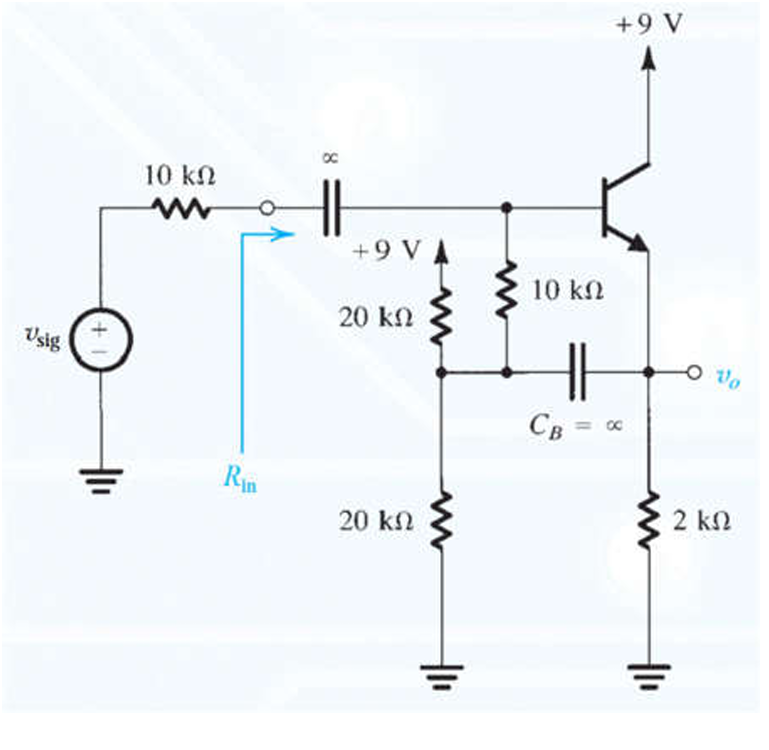
\includegraphics[width=.8\linewidth]{./my-chapters/my-images/Question4/Debai.png}
\end{figure}

\answer{a}{Tìm điểm hoạt động Q của BJT}

\noindent Xét hoạt động chế độ DC cho toàn mạch.

\begin{itemize}[label=-]
	\item Tìm giá trị $V_{BE}$ của BJT trong Multisim
	
	\begin{figure}[H]
		\centering
		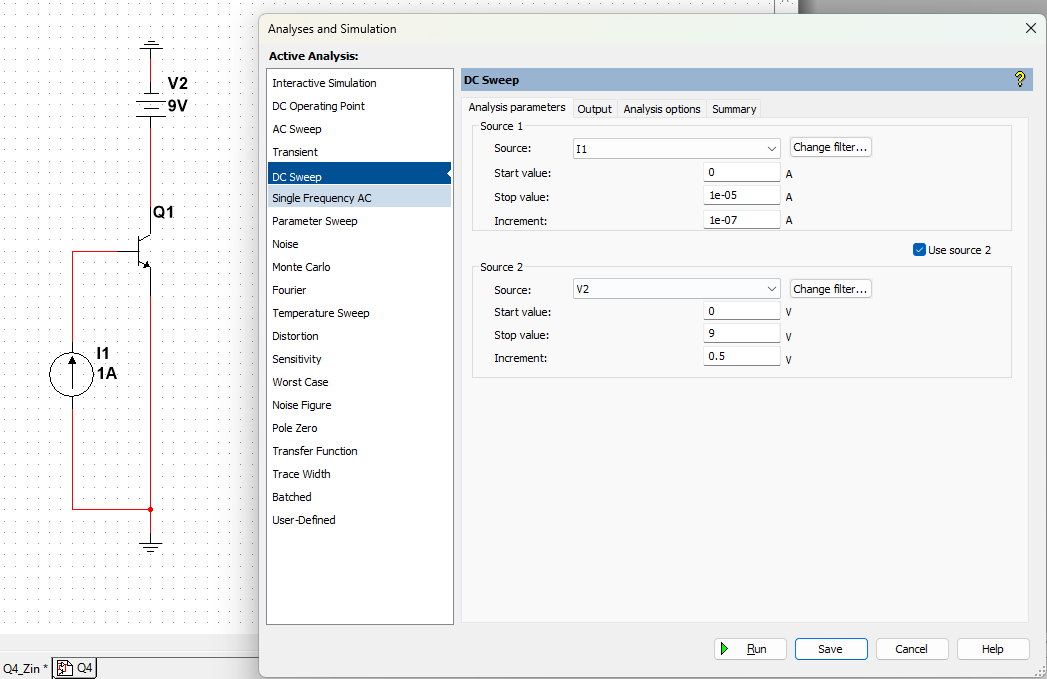
\includegraphics[width=.8\linewidth]{./my-chapters/my-images/Question4/a_doVBE.png}
		\caption{Tìm giá trị $V_{BE}$ của mạch.}
	\end{figure}
	
	Ta sử dụng một chế độ DC Sweep để tìm giá trị $V_{BE}$ dẫn của mạch. Sau khi chạy tool ta có kết quả như sau,
	
	\begin{figure}[H]
		\centering
		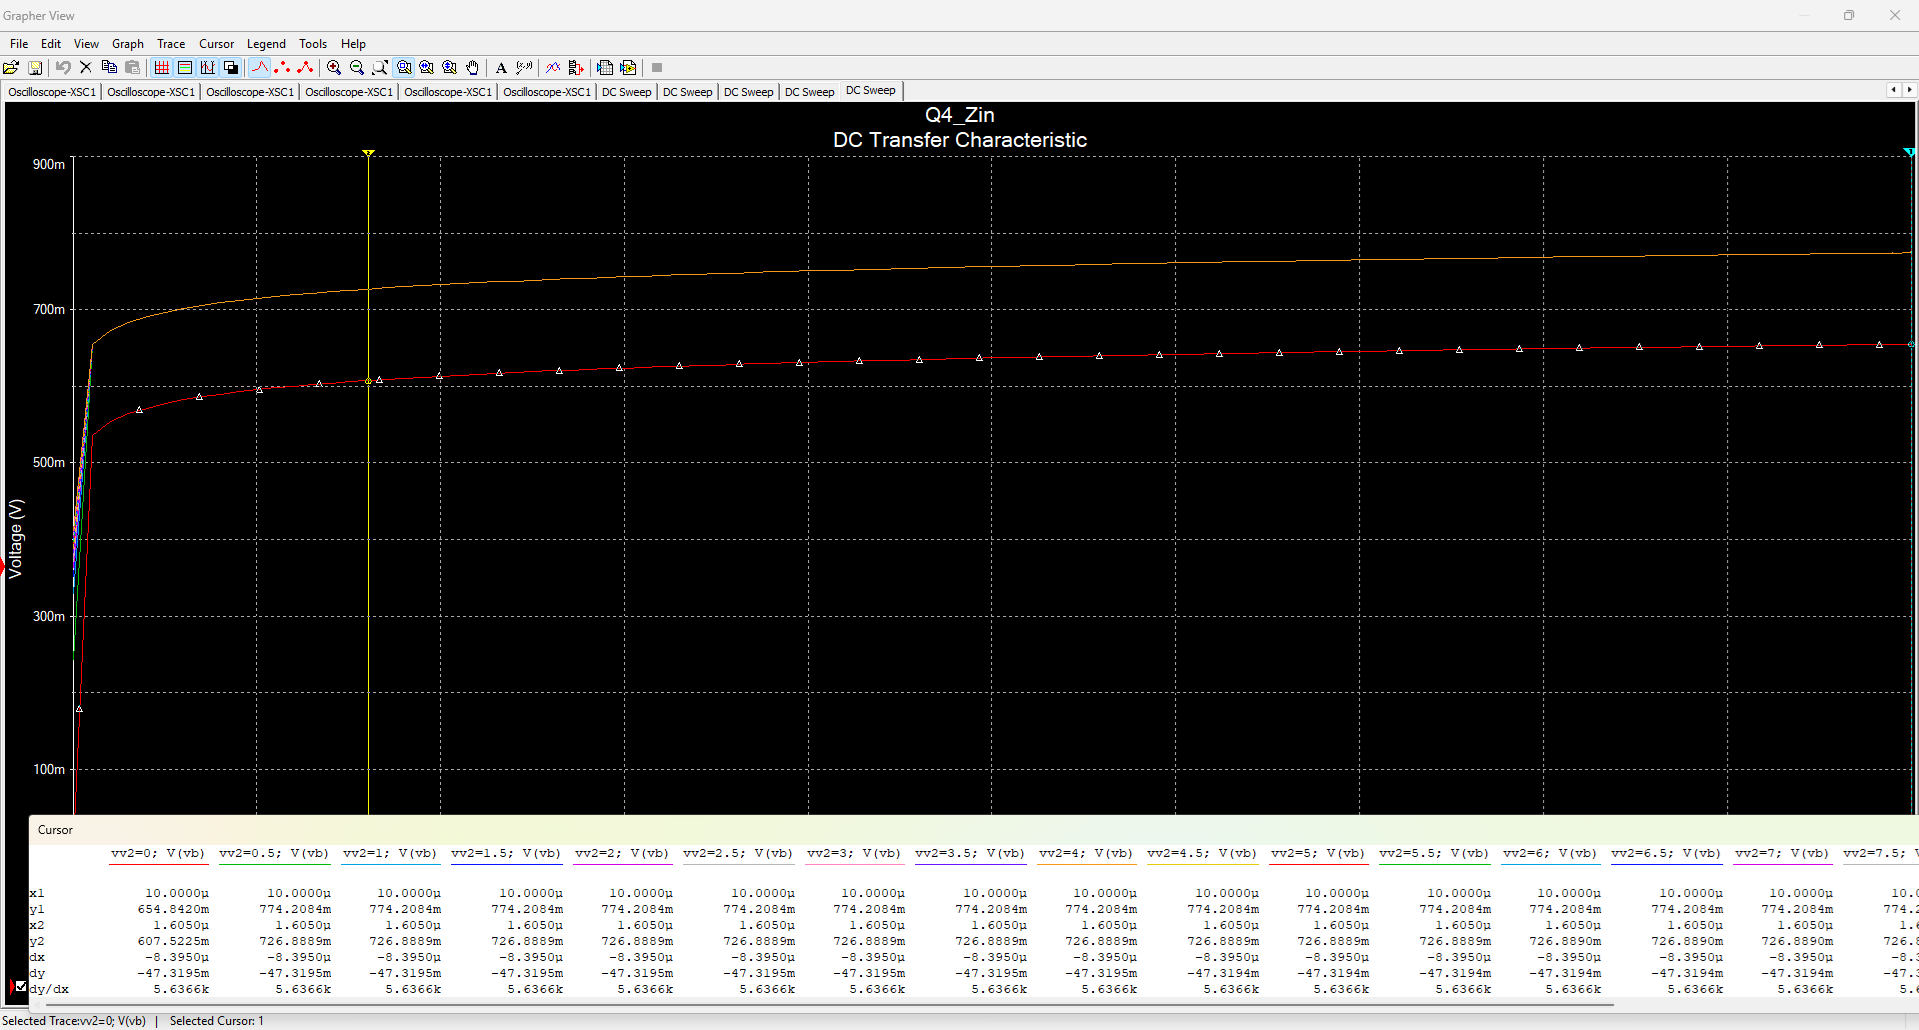
\includegraphics[width=.8\linewidth]{./my-chapters/my-images/Question4/a_timVBE.png}
		\caption{Kết quả sau khi chạy DC Sweep để tìm $V_{BE}$.}
	\end{figure}
	
	Nhìn vậy hình ta thấy được điện áp $V_{BE}$ của BJT dẫn rơi vào tầm $ \approx 0.774\,\text{mA}$. Từ đó, nhóm em chọn $V_{BE} = 0.774\,\text{mA}$ cho câu 4.
	
	\item Tìm giá trị $I_{CQ}$
	
	\begin{figure}[H]
		\centering
		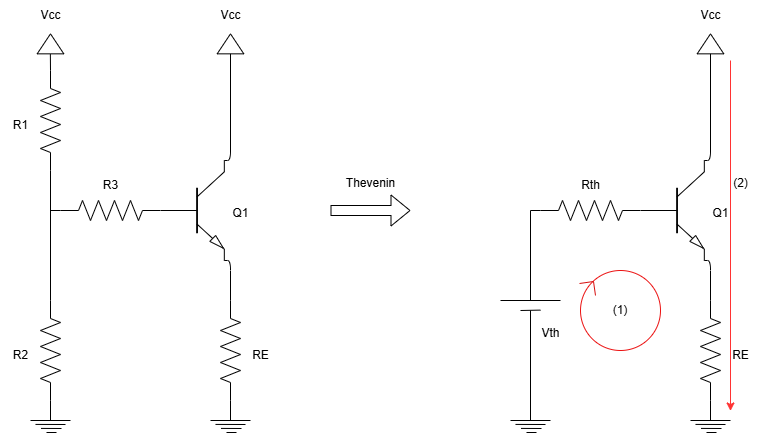
\includegraphics[width=.7\linewidth]{./my-chapters/my-diagrams/Question4/Debai.png}
	\end{figure}
	
	Thevenin ta có:
	\[ R_{th} = R_{3} + R_{1}//R_{2} = 10 + \dfrac{20\times 20}{20 + 20} = 20k\Omega\]
	\[ V_{th} = \dfrac{R_{2}}{R_{1} + R_{2}} V_{cc} = \dfrac{20}{20+20} \times 9 = 4.5V\]
	
	Áp dụng KCL cho vòng (1):
	\[ -V_{th} + I_{B}R_{th} + V_{BE} + I_{E}R_{E} = 0\]
	Ta có: $ I_{E} = (\beta + 1)I_{B} $
	\[\Rightarrow I_{B} = \dfrac{V_{th} - V_{BE}}{R_{th} + (\beta + 1)R_{E}} = \dfrac{4.5 - 0.774}{20 + (100+1)\times 2} = 0.0168\,\text{mA}\]
	Ta có: $I_{C} = \beta I_{B} = 100\times 0.0168\,\text{mA} = 1.68\,\text{mA}$.
	
	\item Tìm giá trị $V_{CEQ}$
	
	Áp dụng KCL cho vòng (2):
	\[ -V_{cc} + V_{CE} + I_{E}R_{E} = 0\]
	Ta có: $I_{C} = \dfrac{\beta}{\beta + 1}I_{E} = \alpha I_{E} \approx I_{E}$
	\[\Rightarrow V_{CE} = V_{cc} - I_{C}R_{E} = 9 - 1.71\times 2 = 5.64V \]
	
	Vậy điểm làm việc Q của tâng 2 là : \finalresult{(I_{CQ}, V_{CEQ}) = (1.68\,\text{\,\text{mA}}, 5.64\,\text{V})}.
	
	\item Kiểm chứng kết quả:
	
	\begin{figure}[H]
		\centering
		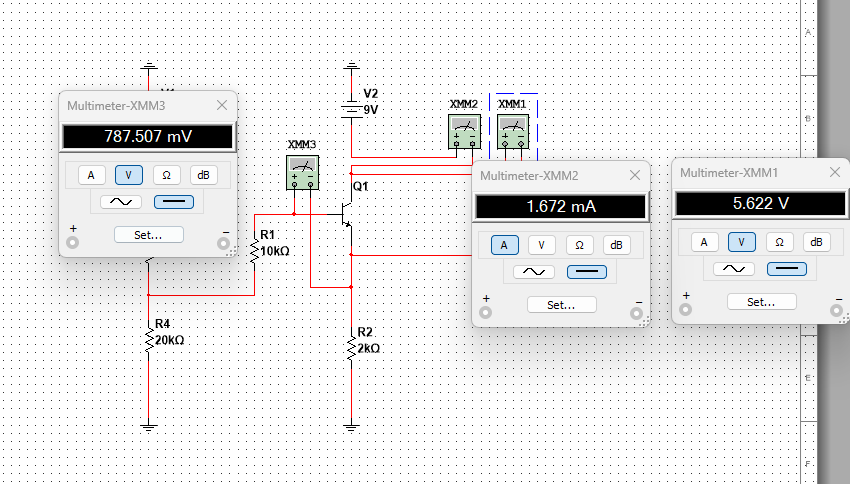
\includegraphics[width=.8\linewidth]{./my-chapters/my-images/Question4/phancucDC_Q.png}
		\caption{Kết quả điểm Q của bài 4.}
	\end{figure}
\end{itemize}

\answer{b}{Đặt $v_{s} = V_{s}\sin \left(\omega t\right)$ vào mạch. Ngõ ra nối với tải $R_{L} = 1k\Omega$. Tìm $A_{vo}$, $G_{v}$, $R_{i}$, $R_{o}$ của mạch.}

\noindent Xét hoạt động chế độ AC cho toàn mạch.

\begin{figure}[H]
	\centering
	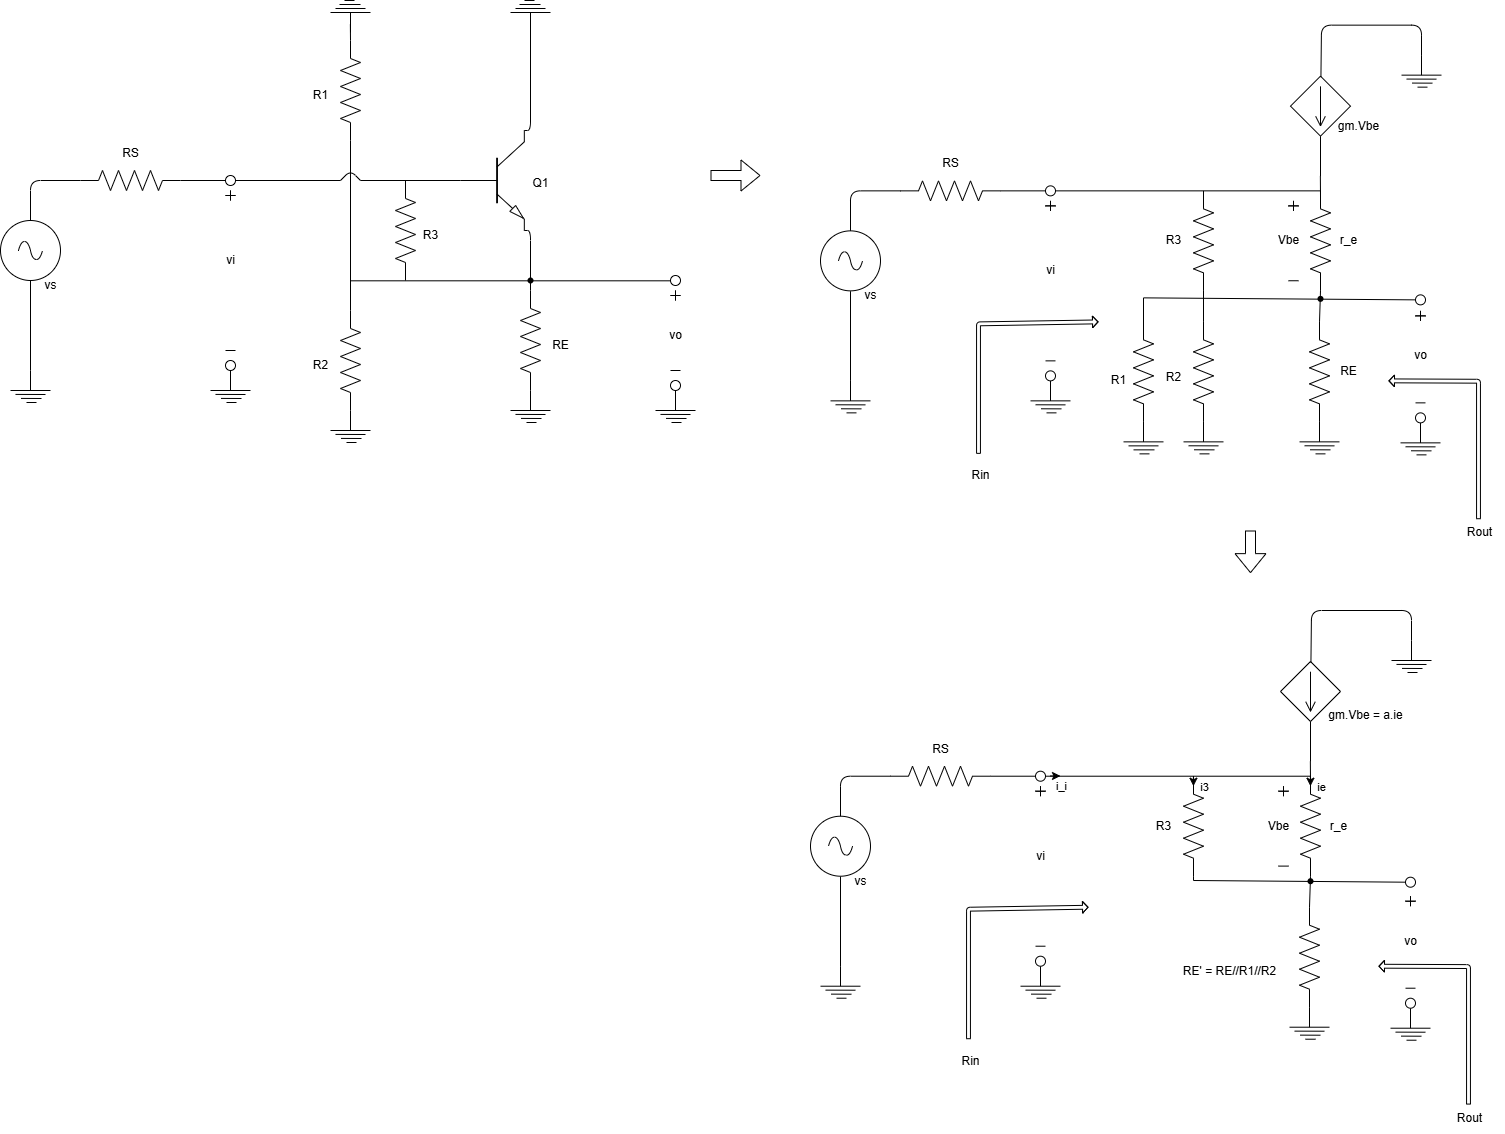
\includegraphics[width=.9\linewidth]{./my-chapters/my-diagrams/Question4/caub_t.png}
\end{figure}

Ta có, 

\begin{itemize}[label=+, leftmargin=2cm]
	\item $R_{E}^{'} = R_{E} // R_{1} // R_{2} \approx 1.6667\,\text{k}\Omega$
	\item $g_{m} = \dfrac{I_{C}}{V_{T}} =  \dfrac{1.68\,\text{m}}{25\,\text{m}} = 67.2mS$
	\item $r_{e} = \dfrac{V_{T}}{I_{E}} = \dfrac{V_{T}}{I_{C}/\alpha} = \dfrac{25\,\text{mV}}{1.68\,\text{mA} / \dfrac{100}{100+1}} \approx 14.7336\,\Omega$
	\item $r_{\pi} = \beta \dfrac{V_{T}}{I_{C}} = 100\times\dfrac{25\,\text{m}}{1.68\,\text{m}} = 1.4881\,\text{k}\Omega$
\end{itemize}

\begin{itemize}[label=-]
	\item Tính giá trị $R_{in}$
	
	Ta có, $R_{in} = \dfrac{v_{i}}{i_{i}}\bigg|_{i_{o} = 0}$, đầu tiên ta xét
	
	\begin{itemize}[label=+, leftmargin=1cm]
		\item $i_{i} = i_{3} + i_{e} - \alpha i_{e} $
		
		Trong đó, $i_{3} = \dfrac{i_{e} r_{e}}{R_{3}}$
		
		$\Rightarrow i_{i} = \dfrac{i_{e} r_{e}}{R_{3}} + i_{e}(1-\alpha)$
		\item $v_{i} = v_{be} + v_{o}$
		
		Trong đó, $v_{o} = R_{E}^{'} (i_{3} + i_{e}) = R_{E}^{'} \left( \dfrac{i_{e} r_{e}}{R_{3}} + i_{e} \right)$
	\end{itemize}
	
	$\Rightarrow R_{in} = \dfrac{R_{E}^{'} \left( \dfrac{i_{e} r_{e}}{R_{3}} + i_{e} \right) + i_{e}r_{e}}{\dfrac{i_{e} r_{e}}{R_{3}} + i_{e}(1-\alpha)} = \dfrac{R_{E}^{'} \left( \dfrac{r_{e}}{R_{3}} + 1 \right) + r_{e}}{\dfrac{r_{e}}{R_{3}} + (1-\alpha)} \approx 148.0428 \,\text{k}\Omega$.
	
	$\Rightarrow$ \finalresult{R_{in} = 148.0428\,\text{k}\Omega}.
	
	\item Tính giá trị $R_{out}$
	
	Ta có, $R_{out} = \dfrac{v_{o}}{i_{o}}\bigg|_{v_{i} = 0}$
	
	$\Rightarrow R_{out} = R_{E}^{'} // r_{e} // \dfrac{R_{3}}{\beta + 1} = 12.7272\,\Omega$.
	
	$\Rightarrow$ \finalresult{R_{out} = 12.7272\,\Omega}.
	
	\item Tính giá trị $A_{vo}$
	
	Ta có, $A_{vo} = \dfrac{v_{o}}{v_{i}}\bigg|_{R_{L} = \infty} = \dfrac{R_{E}^{'} \left( \dfrac{r_{e}}{R_{3}} + 1 \right)}{R_{E}^{'} \left( \dfrac{r_{e}}{R_{3}} + 1 \right) + r_{e}} \approx 0.9913 \,\text{V/V}$.
	
	$\Rightarrow$ \finalresult{A_{vo} = 0.9913 \,\text{V/V}}.
	
	\item Tính giá trị $G_{v}$
	
	ta có, $G_{v} = \dfrac{v_{o}}{v_{s}} = \dfrac{R_{in}}{R_{in} + R_{s}} A_{v} = \dfrac{148.0428}{148.0428 + 10}\times 0.9914 \approx 0.9287 \,\text{V/V}$.
	
	$\Rightarrow$ \finalresult{G_{v} = 0.9287 \,\text{V/V}}. 
	
	\item Kiểm tra kết quả
	
	\begin{figure}[H]
		\centering
		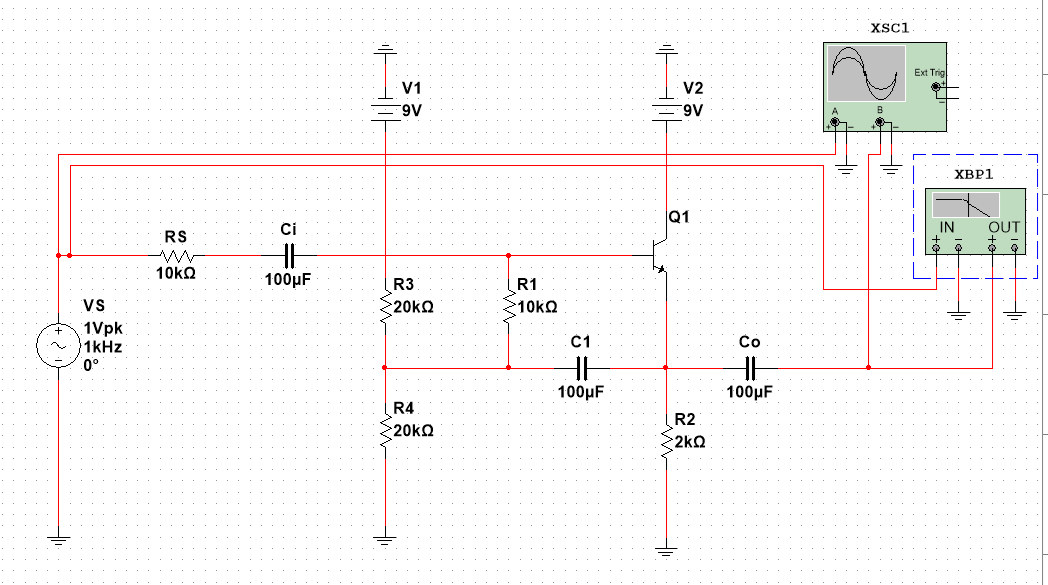
\includegraphics[width=.8\linewidth]{./my-chapters/my-images/Question4/b_GV_test.png}
	\end{figure}
	
	\begin{figure}[H]
		\centering
		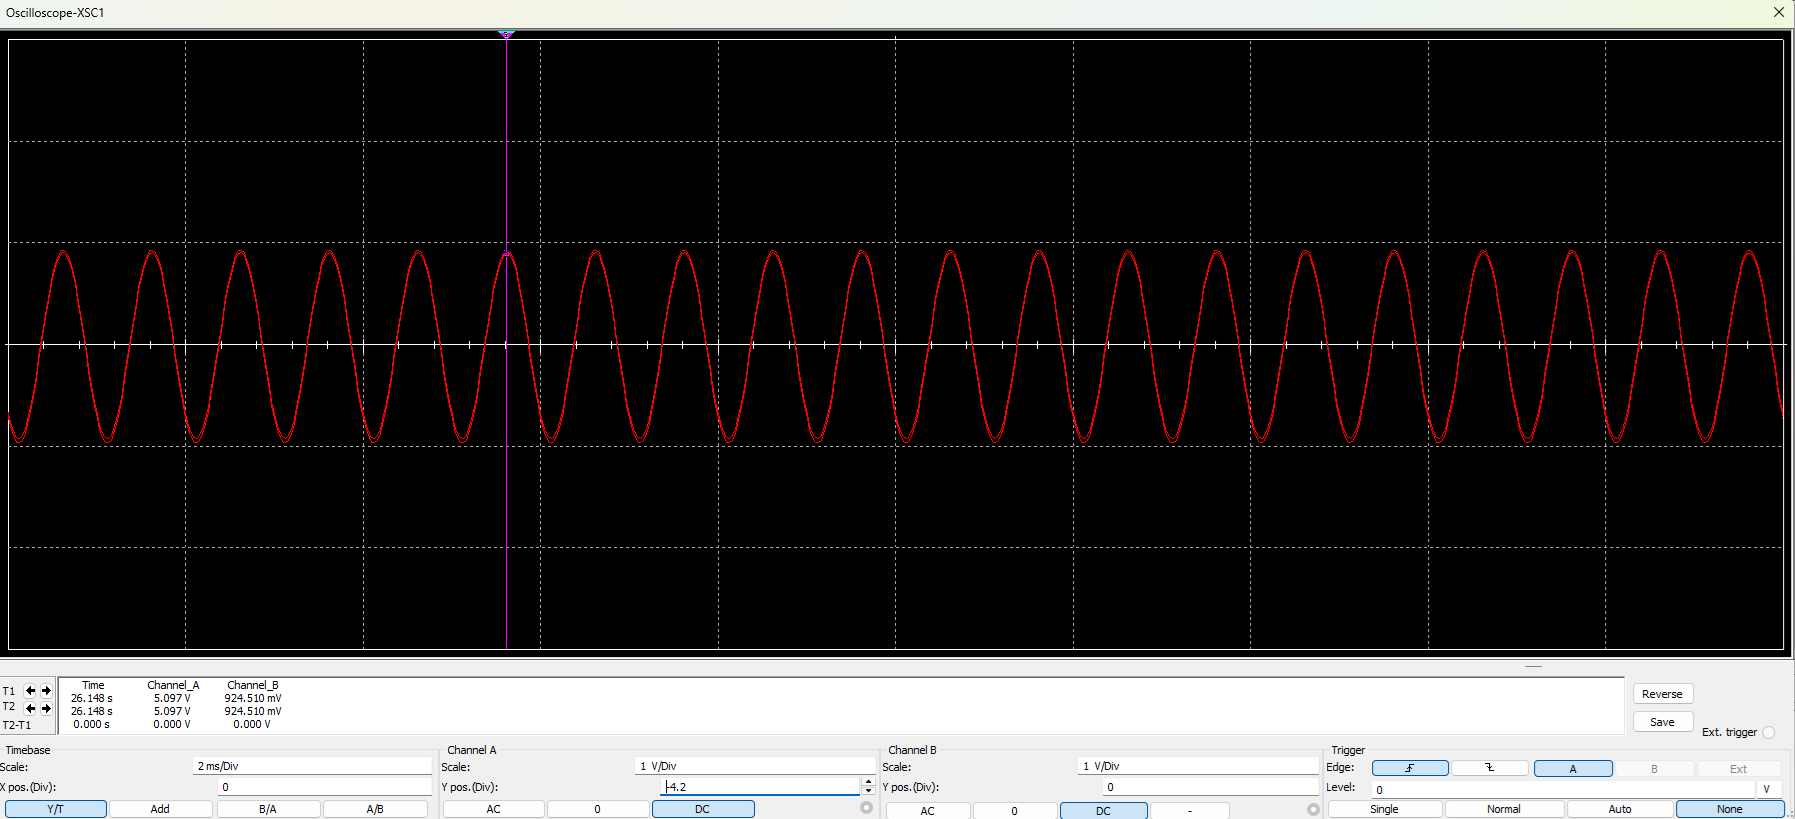
\includegraphics[width=.8\linewidth]{./my-chapters/my-images/Question4/b_Avo_wave.png}
		\caption{Coi dạng sóng ngõ vào và ngõ ra của mạch.}
	\end{figure}
	
	\begin{figure}[H]
		\centering
		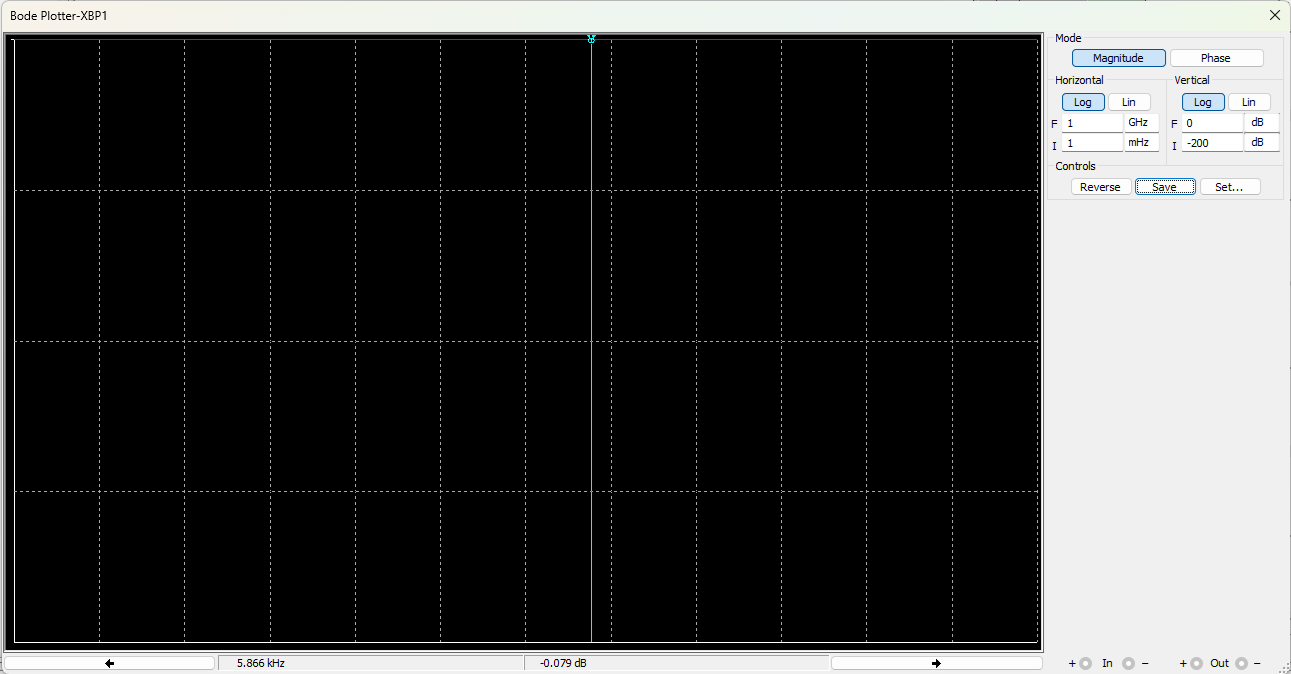
\includegraphics[width=.8\linewidth]{./my-chapters/my-images/Question4/b_Avo_bode.png}
		\caption{Tiến hành đo $A_{vo} = -0.079dB \approx 0.9909$.}
	\end{figure}
	
	\begin{figure}[H]
		\centering
		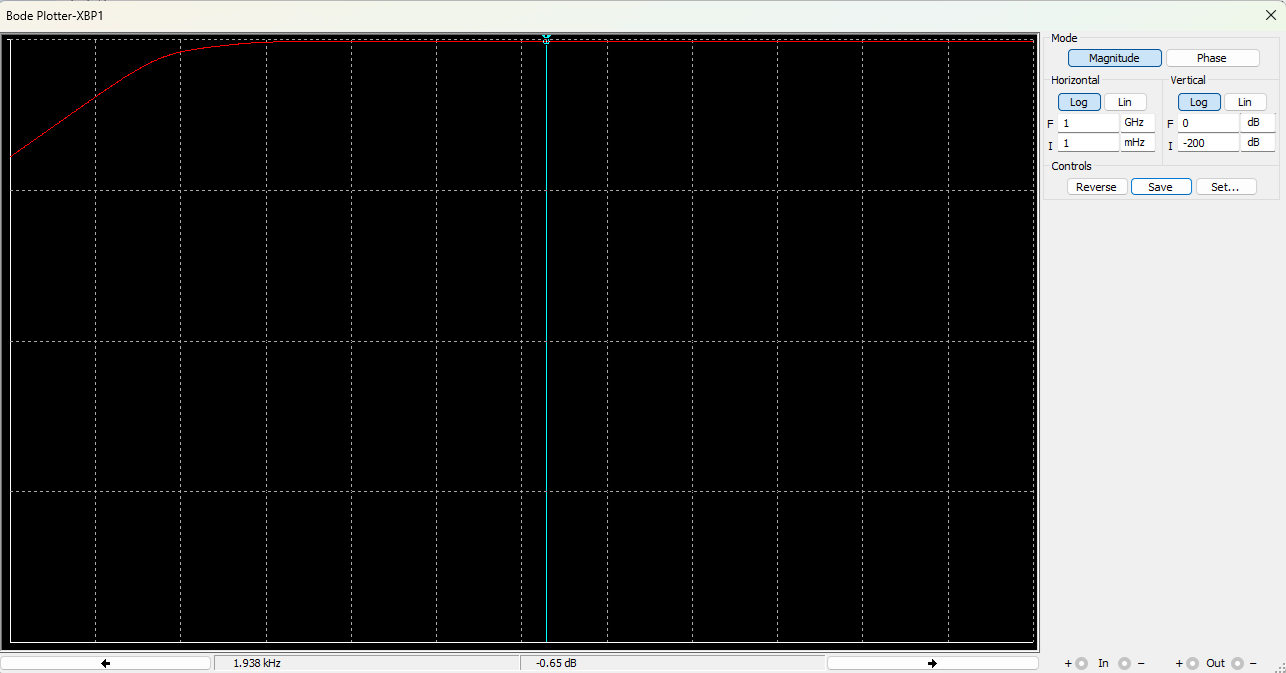
\includegraphics[width=.8\linewidth]{./my-chapters/my-images/Question4/b_GV_bode.png}
		\caption{Tiến hành đo $G_{v} = -0.65dB \approx 0.9279$.}
	\end{figure}
\end{itemize}

\answer{c}{Bỏ tụ $C_{B}$ ra khỏi mạch. Lập lại câu a và b. Từ đó, nêu vai trò của tụ $C_{B}$.}

\begin{figure}[H]
	\centering
	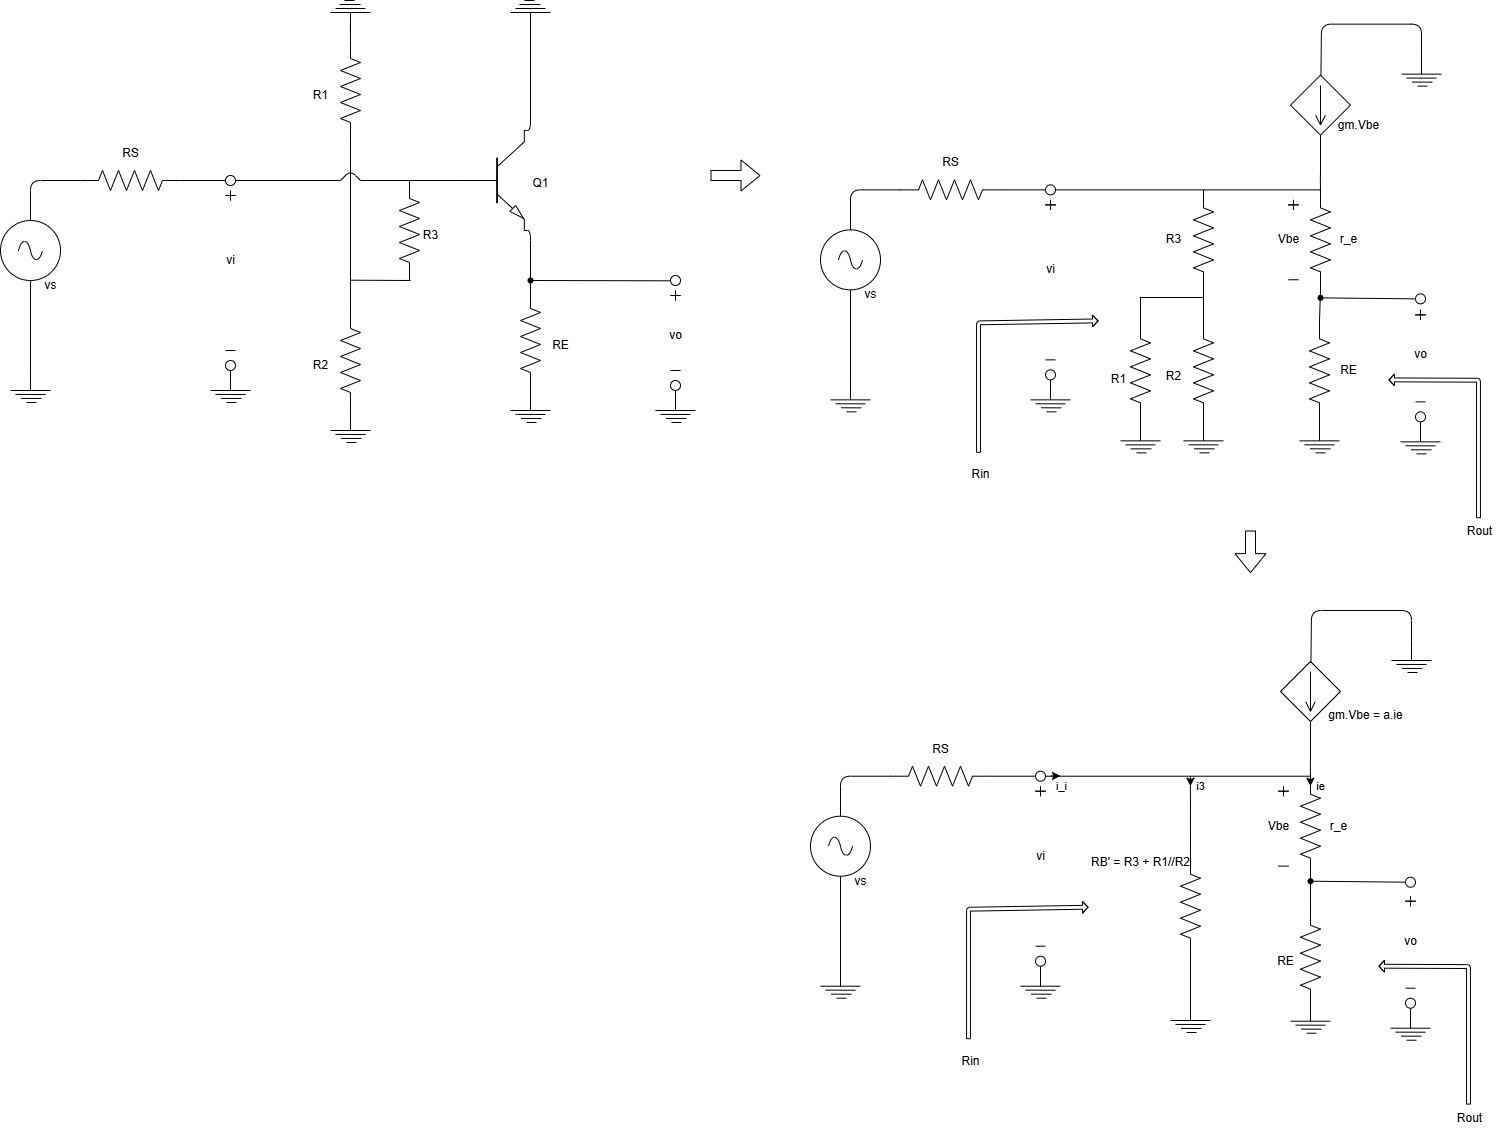
\includegraphics[width=.9\linewidth]{./my-chapters/my-diagrams/Question4/cauc_t.png}
\end{figure}

Ta có, 

\begin{itemize}[label=+, leftmargin=2cm]
	\item $R_{B}^{'} = R_{3} + R_{1} // R_{2} = 20\,\text{k}\Omega$
	\item $g_{m} = \dfrac{I_{C}}{V_{T}} =  \dfrac{1.68\,\text{m}}{25\,\text{m}} = 67.2mS$
	\item $r_{e} = \dfrac{V_{T}}{I_{E}} = \dfrac{V_{T}}{I_{C}/\alpha} = \dfrac{25\,\text{mV}}{1.68\,\text{mA} / \dfrac{100}{100+1}} \approx 14.7336\,\Omega$
	\item $r_{\pi} = \beta \dfrac{V_{T}}{I_{C}} = 100\times\dfrac{25\,\text{m}}{1.68\,\text{m}} = 1.4881\,\text{k}\Omega$
\end{itemize}

\begin{itemize}[label=-]
	\item Tính giá trị $R_{in}$
	
	Ta có, $R_{in} = \dfrac{v_{i}}{i_{i}}\bigg|_{i_{o} = 0}$

	\[ \rightarrow R_{in} = R_{B}^{'} // (\beta + 1)(r_{e} + R_{E}) \approx 18.2102\,\text{k}\Omega \]
	$\Rightarrow$ \finalresult{R_{in} = 18.2102\,\text{k}\Omega}.
	
	\item Tính giá trị $R_{out}$
	
	Ta có, $R_{out} = \dfrac{v_{o}}{i_{o}}\bigg|_{v_{i} = 0}$ 
	
	\[\rightarrow R_{out} = R_{E} // r_{e} = 14.6259\,\Omega \]
	$\Rightarrow$ \finalresult{R_{out} = 14.6259\,\Omega}.
	
	\item Tính giá trị $A_{vo}$
	
	Ta có, $A_{vo} = \dfrac{v_{o}}{v_{i}}\bigg|_{R_{L} = \infty} = \dfrac{R_{E}}{R_{E} + r_{e}} \approx 0.9927\,\text{V/V}$.
	
	$\Rightarrow$ \finalresult{A_{vo} \approx 0.9927\,\text{V/V}}.
	
	\item Tính giá trị $G_{v}$
	
	ta có, $G_{v} = \dfrac{v_{o}}{v_{s}} = \dfrac{R_{in}}{R_{in} + R_{s}} A_{v} = \dfrac{18.2102}{18.2102 + 10}\times 0.9927 \approx 0.6408 \,\text{V/V}$.
	
	$\Rightarrow$ \finalresult{G_{v} = 0.6408 \,\text{V/V}}. 
	
	\item Kiểm tra kết quả
	
	\begin{figure}[H]
		\centering
		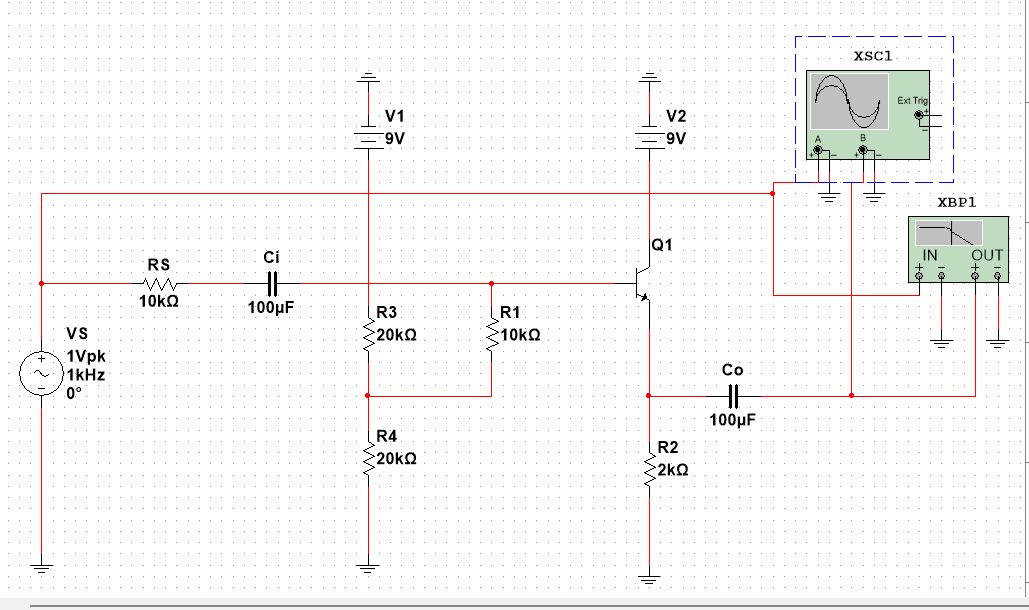
\includegraphics[width=.8\linewidth]{./my-chapters/my-images/Question4/cauc_test.png}
	\end{figure}
	
	\begin{figure}[H]
		\centering
		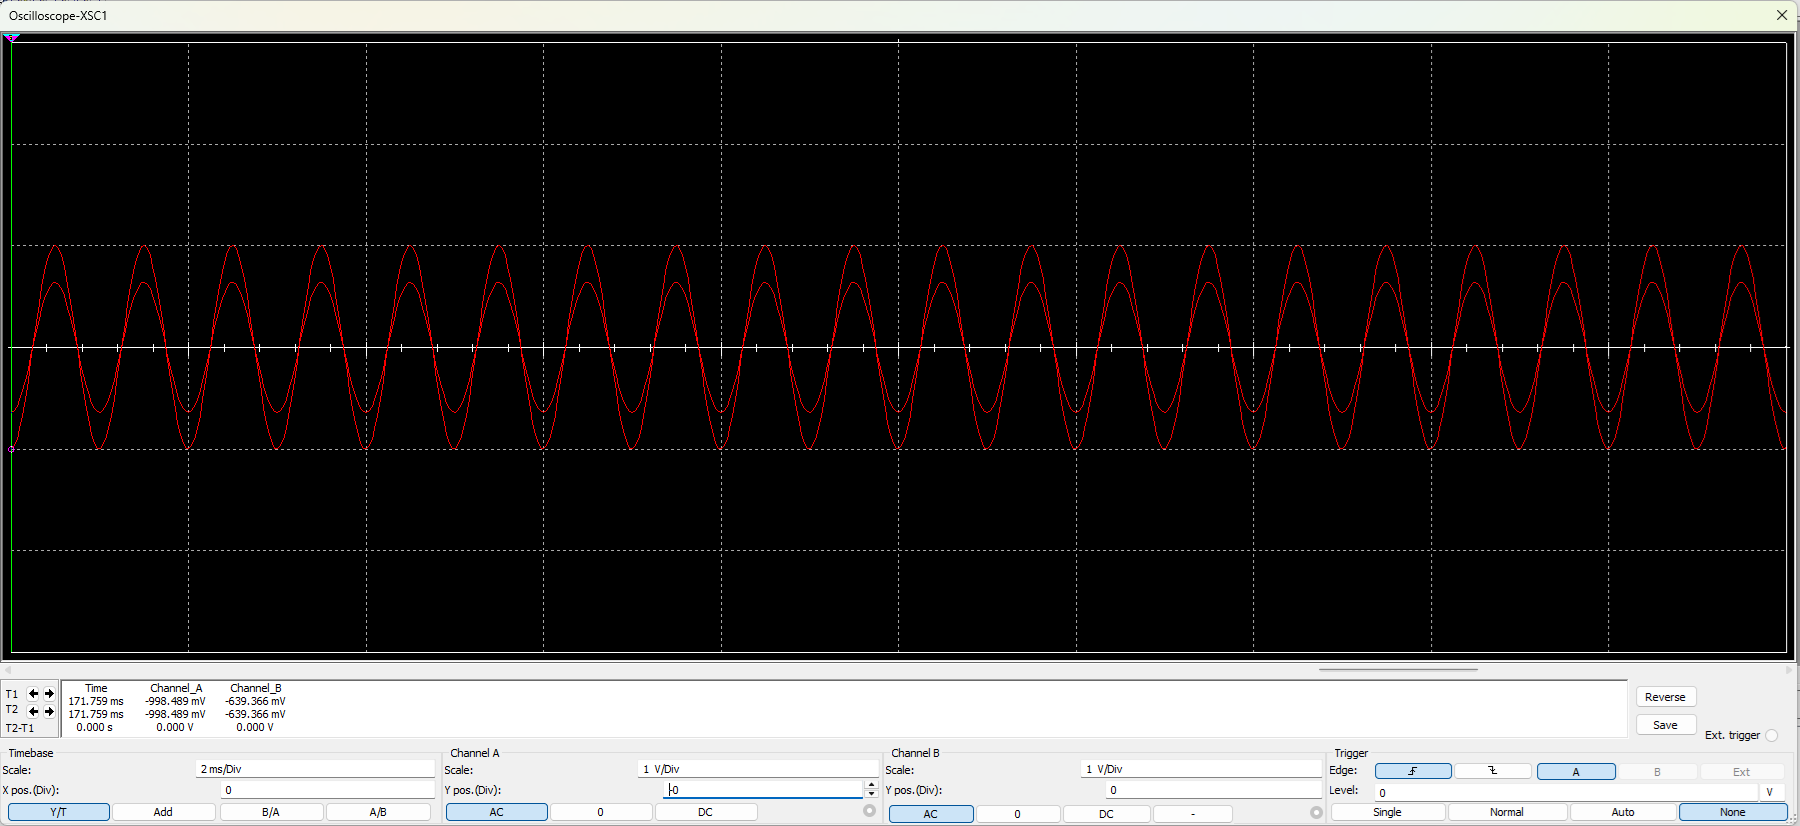
\includegraphics[width=.8\linewidth]{./my-chapters/my-images/Question4/cauc_wave.png}
		\caption{Coi dạng sóng ngõ vào và ngõ ra của mạch.}
	\end{figure}
	
	\begin{figure}[H]
		\centering
		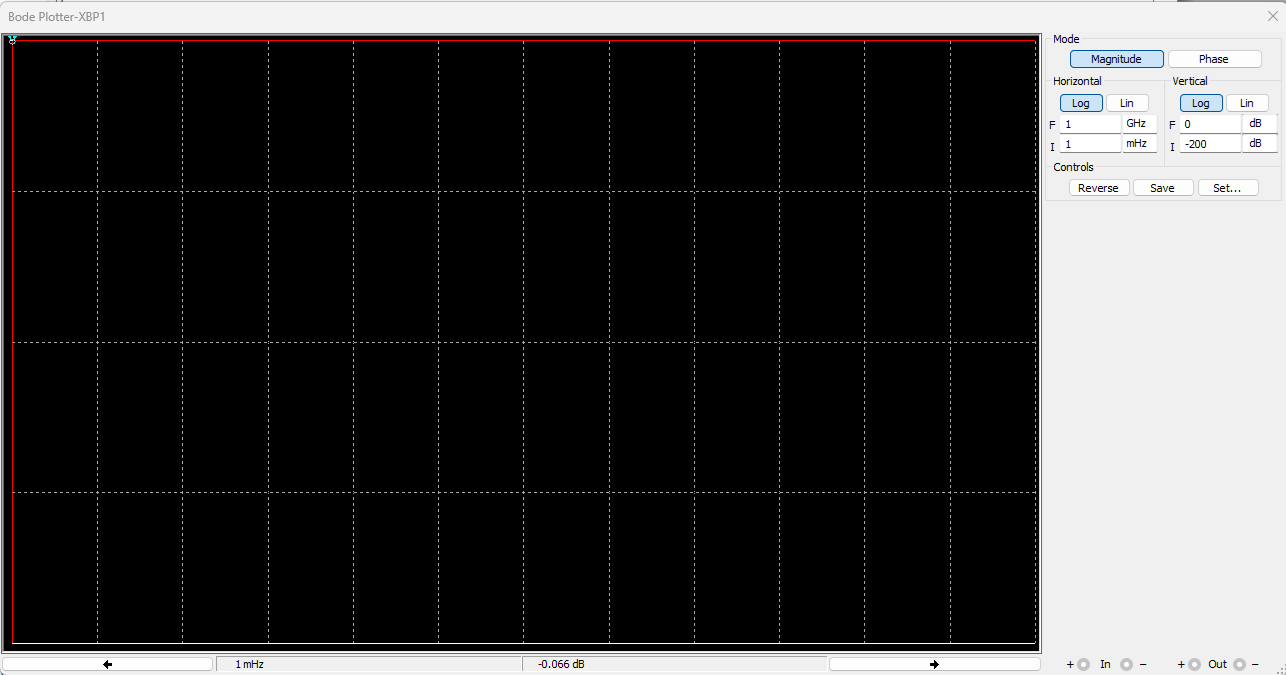
\includegraphics[width=.8\linewidth]{./my-chapters/my-images/Question4/cau_c_bode_avo.png}
		\caption{Tiến hành đo $A_{vo} = -0.066dB \approx 0.9924$.}
	\end{figure}
	
	\begin{figure}[H]
		\centering
		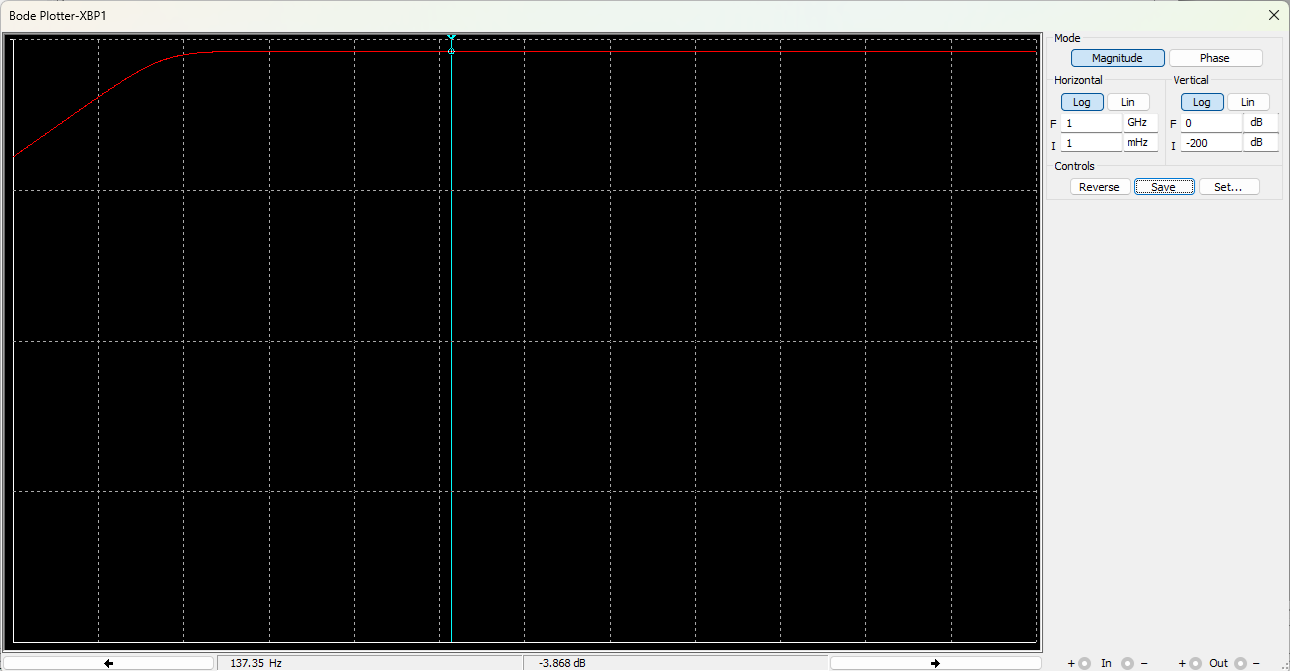
\includegraphics[width=.8\linewidth]{./my-chapters/my-images/Question4/cau_c_bode_gv.png}
		\caption{Tiến hành đo $G_{v} = -3.868dB \approx 0.6406$.}
	\end{figure}
\end{itemize}

\noindent\textbf{Nhận xét}

Mạch trên giống với mạch Bootstrapped Emitter Follower với có một tự $C_{B}$ hồi tiếp dương qua tụ, mạch giúp tăng điện trở đầu vào giúp tăng độ lợi của mạch mà không cần tăng điện trở lên quá cao. Với một trên chỉ cần hồi tiếp về kết hợp một điện trở $R_{1} = 10 \,\text{k}\Omega$ đã có thể tăng $R_{in}$ từ $18.2102\,\text{k}\Omega \rightarrow 148.0428 \,\text{k}\Omega$ có nghĩa là tăng lên đến tầm $8$ lần, và tăng độ lợi $G_{v}$ từ $0.6408 \rightarrow 0.9287$.
\question{Câu 5}

Cho mạch khuếch đại tín hiệu được ghép liên tầng như hình vẽ. Trong đó, $Q_{1}$ là BJT có $\beta = 100$ và mã 2SC1815, và $Q_{2}$ có $\beta = 80$ có mã là 2N2907.

\begin{figure}[H]
	\centering
	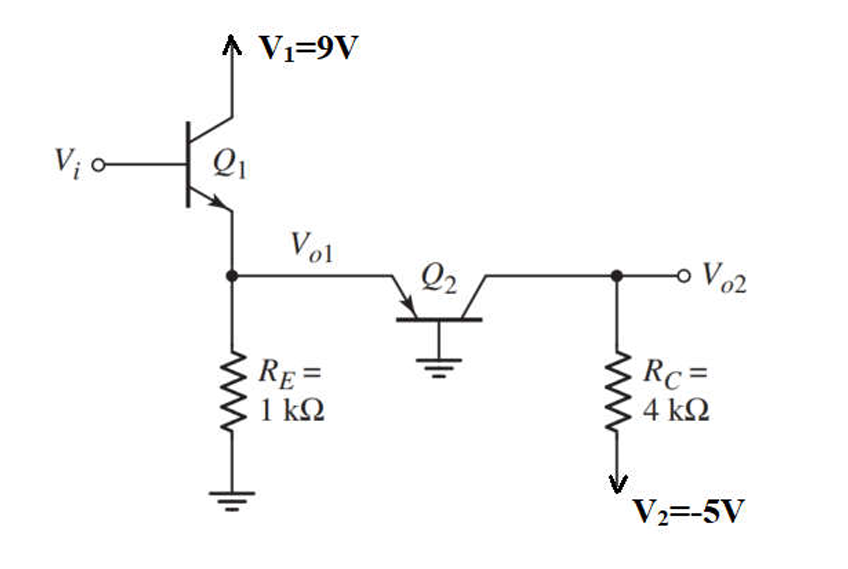
\includegraphics[width=.8\linewidth]{./my-chapters/my-images/Question5/debai.png}
\end{figure}

\answer{a}{Sử dụng phần mềm mô phỏng, vẽ VTC của mạch (ngõ vào $V_{i}$ và ngõ ra là $V_{o}$).}

Sử dụng chế độ DC Sweep trong Multisim để khảo sát VTC,

\begin{figure}[H]
	\centering
	\begin{minipage}{.5\linewidth}
		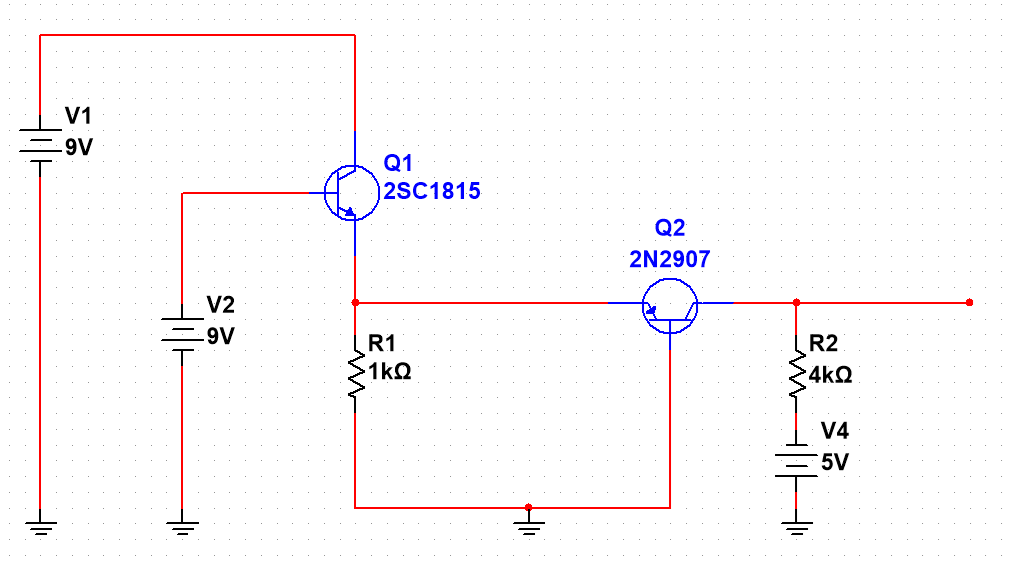
\includegraphics[width=.8\linewidth]{./my-chapters/my-images/Question5/a_mach.png}
	\end{minipage}
	\begin{minipage}{.4\linewidth}
		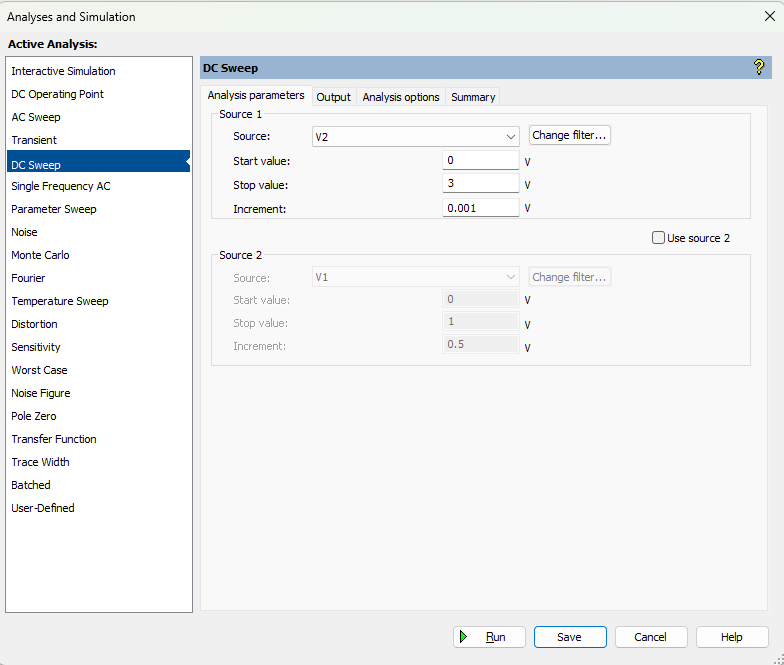
\includegraphics[width=.8\linewidth]{./my-chapters/my-images/Question5/a_dc_sweep.png}
	\end{minipage}
\end{figure}

\begin{figure}[H]
	\centering
	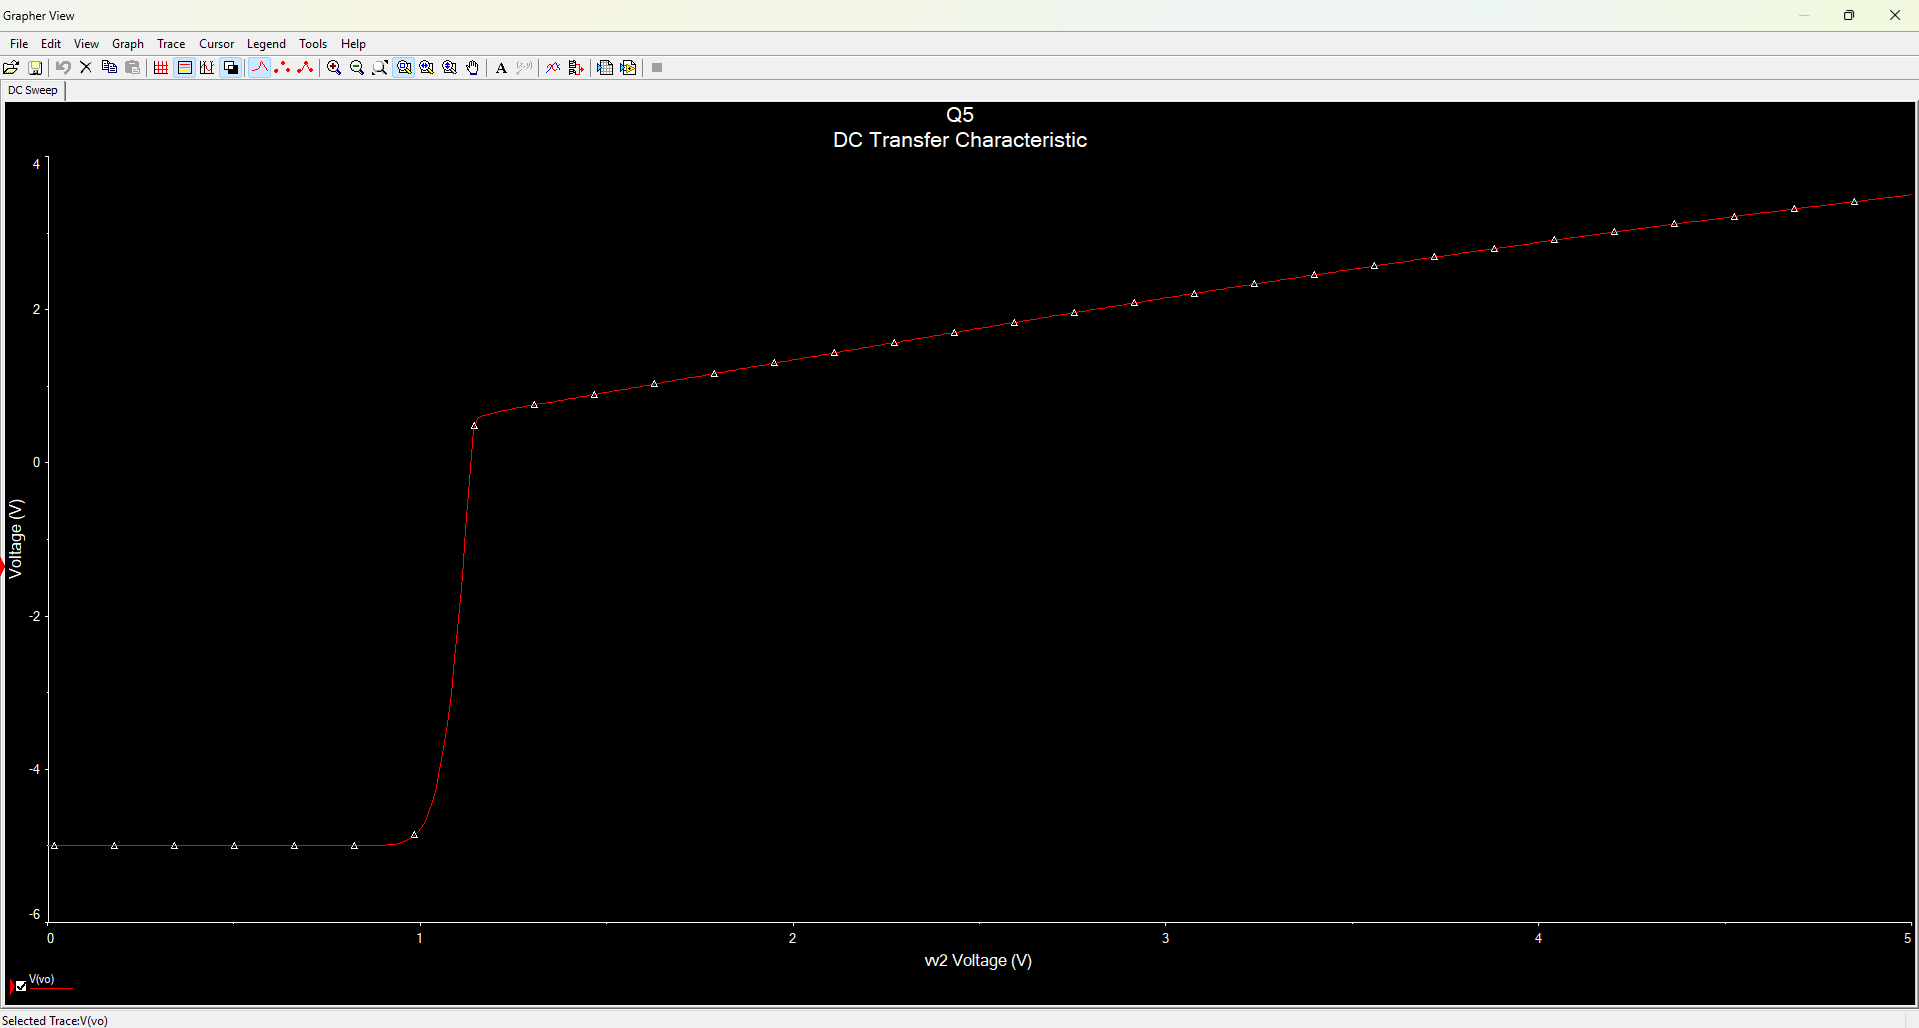
\includegraphics[width=.9\linewidth]{./my-chapters/my-images/Question5/a_VTC.png}
	\caption{VTC của mạch với ngõ vào $V_{i}$ và ngõ ra là $V_{o}$.}
\end{figure}

\begin{minipage}{0.4\linewidth}
	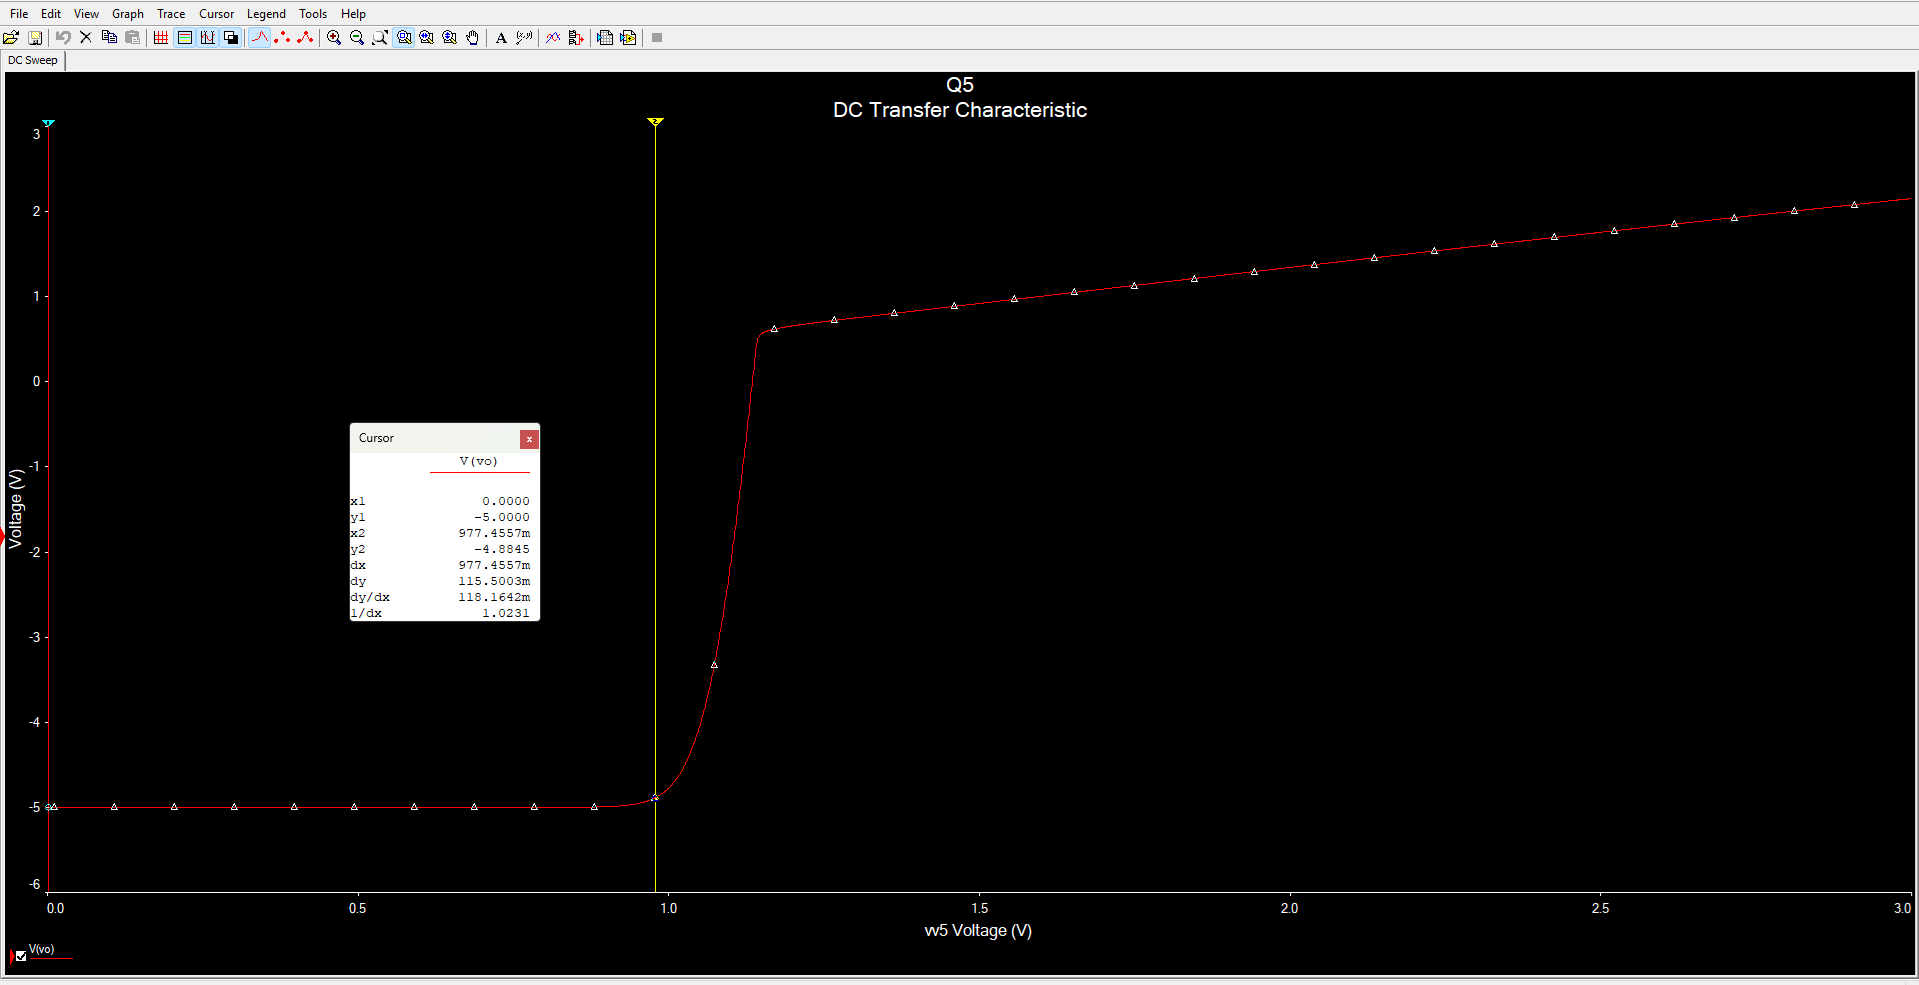
\includegraphics[width=\linewidth]{./my-chapters/my-images/Question5/a_cutoff.png}
\end{minipage}
\begin{minipage}{0.5\linewidth}
	\begin{itemize}[label=-]
		\item Với $V_{i} < 0.9775\,\textsf{V}$ thì mạch bị rơi vào miền cut off, lúc này ngõ ra của mạch luôn bằng $V_{EE} = -5\,\textsf{V}$.
		
		\item Với $0.9775 < V_{i} < 1.1675\,\textsf{V}$ thì mạch trong miền khuếch đại, với độ dốc lớn.
	\end{itemize}
\end{minipage}

\begin{minipage}{0.4\linewidth}
	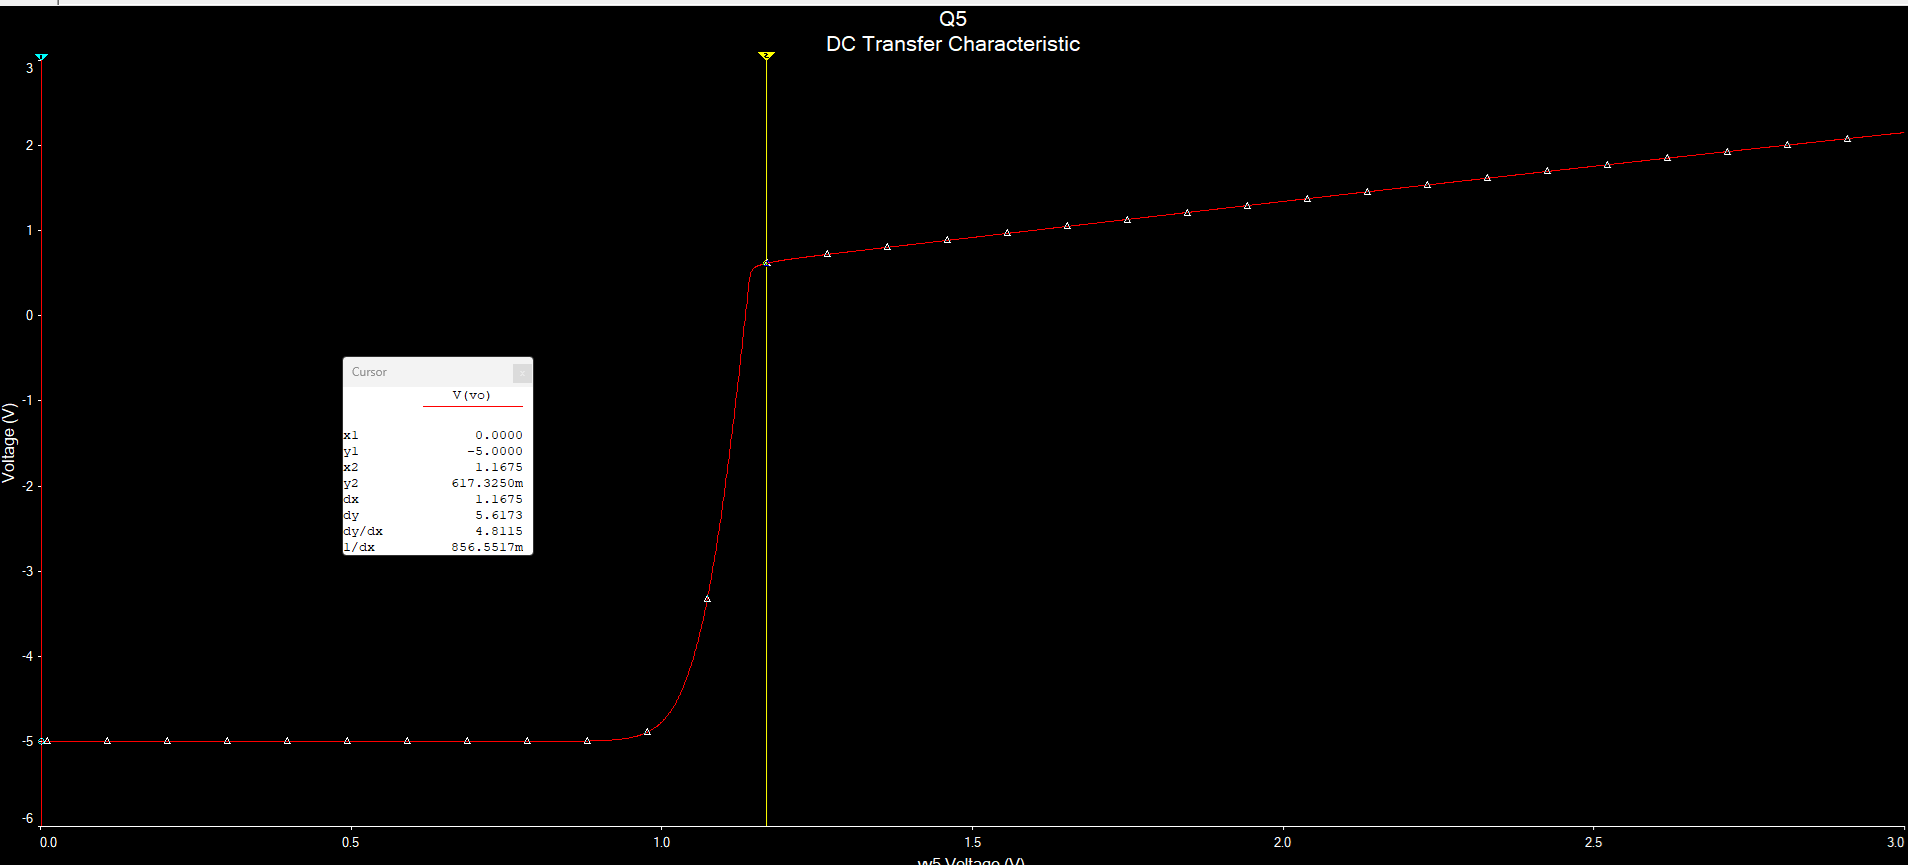
\includegraphics[width=\linewidth]{./my-chapters/my-images/Question5/a_linear.png}
\end{minipage}
\begin{minipage}{0.5\linewidth}
	\begin{itemize}[label=-]
		\item Với $V_{i} > 1.1675\,\textsf{V}$ thì mạch trong miền bão hòa.
	\end{itemize}
\end{minipage}
\answer{b}{Lựa chọn điểm phân cực của cả mạch trên VTC và thiết kế mạch ghép vào phía trước VTC để có được điểm phân cực đó.}

Quan sát VTC của mạch, để tín hiệu ngõ ra không bị méo dạng thì ta chọn điểm $Q$ với $V_{i} = 1.0998\,\text{V}$.

\begin{figure}[H]
	\centering
	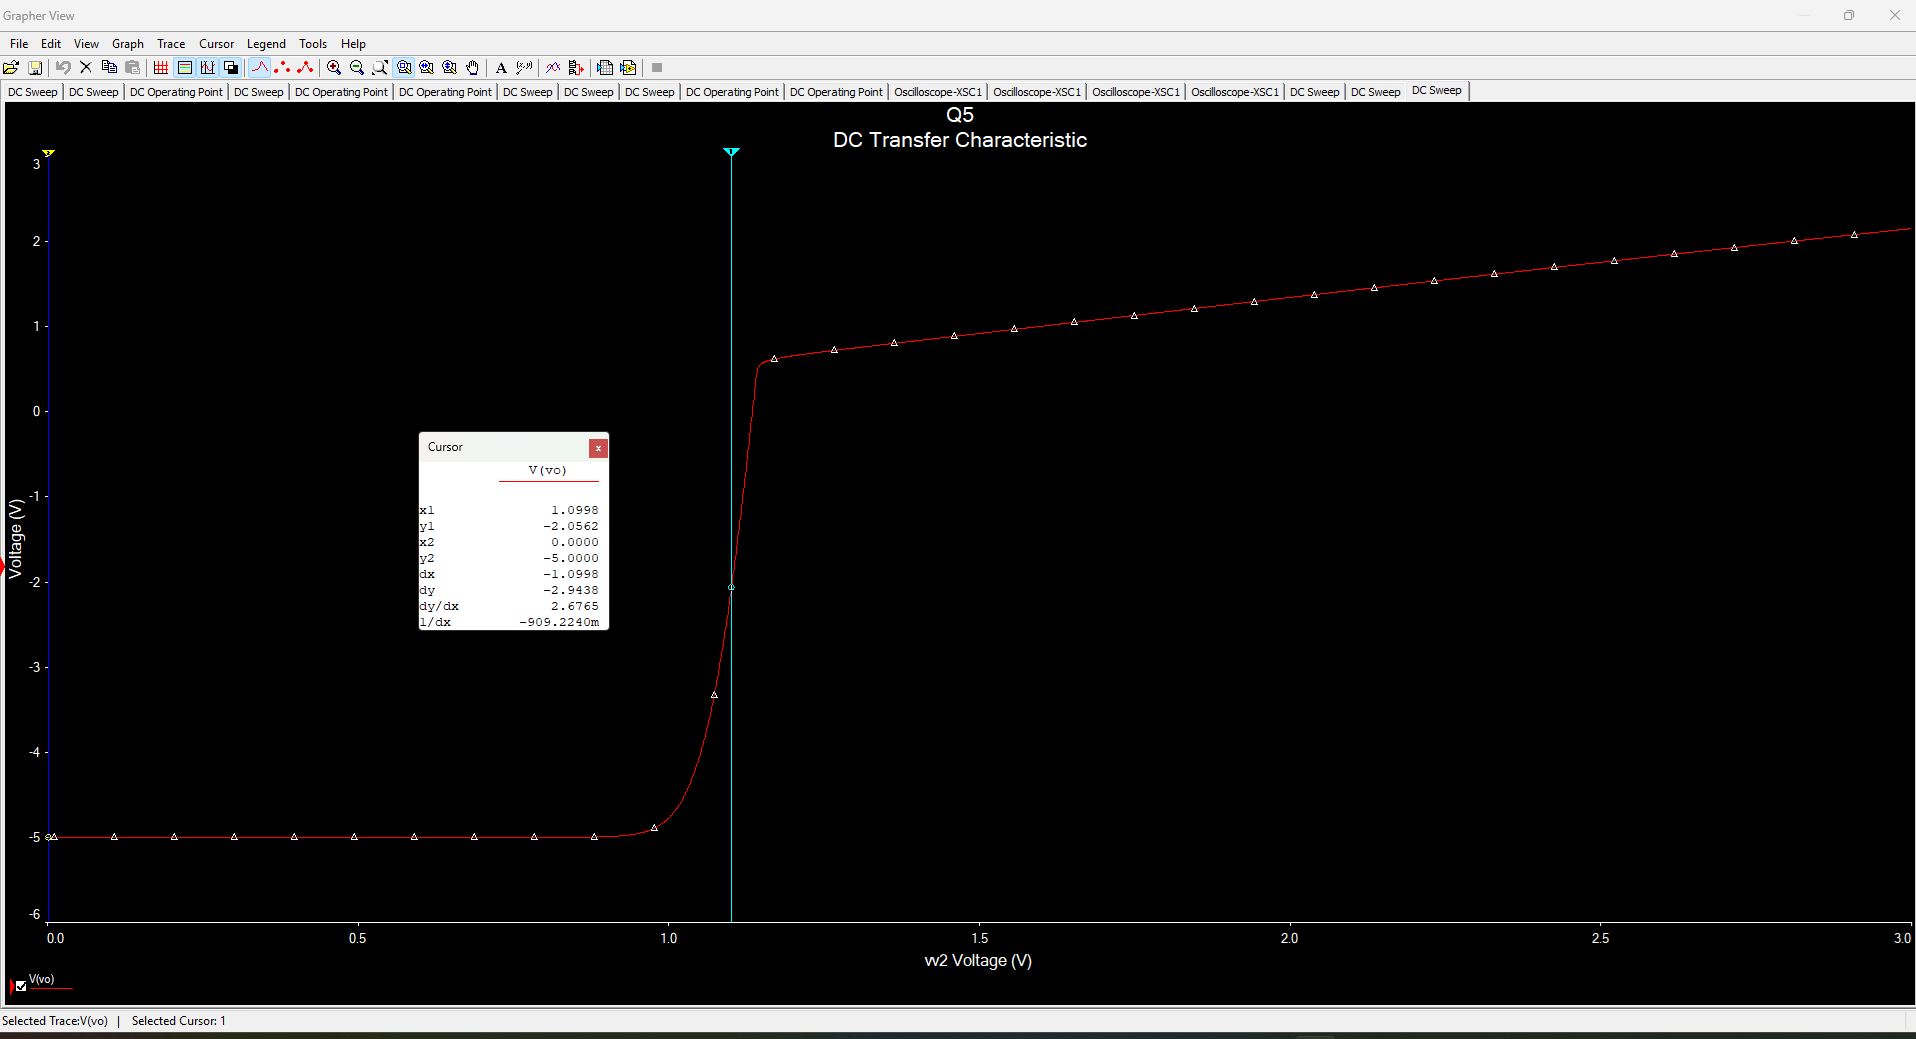
\includegraphics[width=.9\linewidth]{./my-chapters/my-images/Question5/b_Q_tong.png}
	\caption{Điểm hoạt động của toàn mạch rơi vào tầm $V_{i} = 1.0998\,\text{V}$ để tín hiệu $V_{o}$ không méo dạng.}
\end{figure}

Với $V_{i} = 1.0998\,\text{V}$, ta chọn được hai điểm:

\begin{figure}[H]
	\centering
%	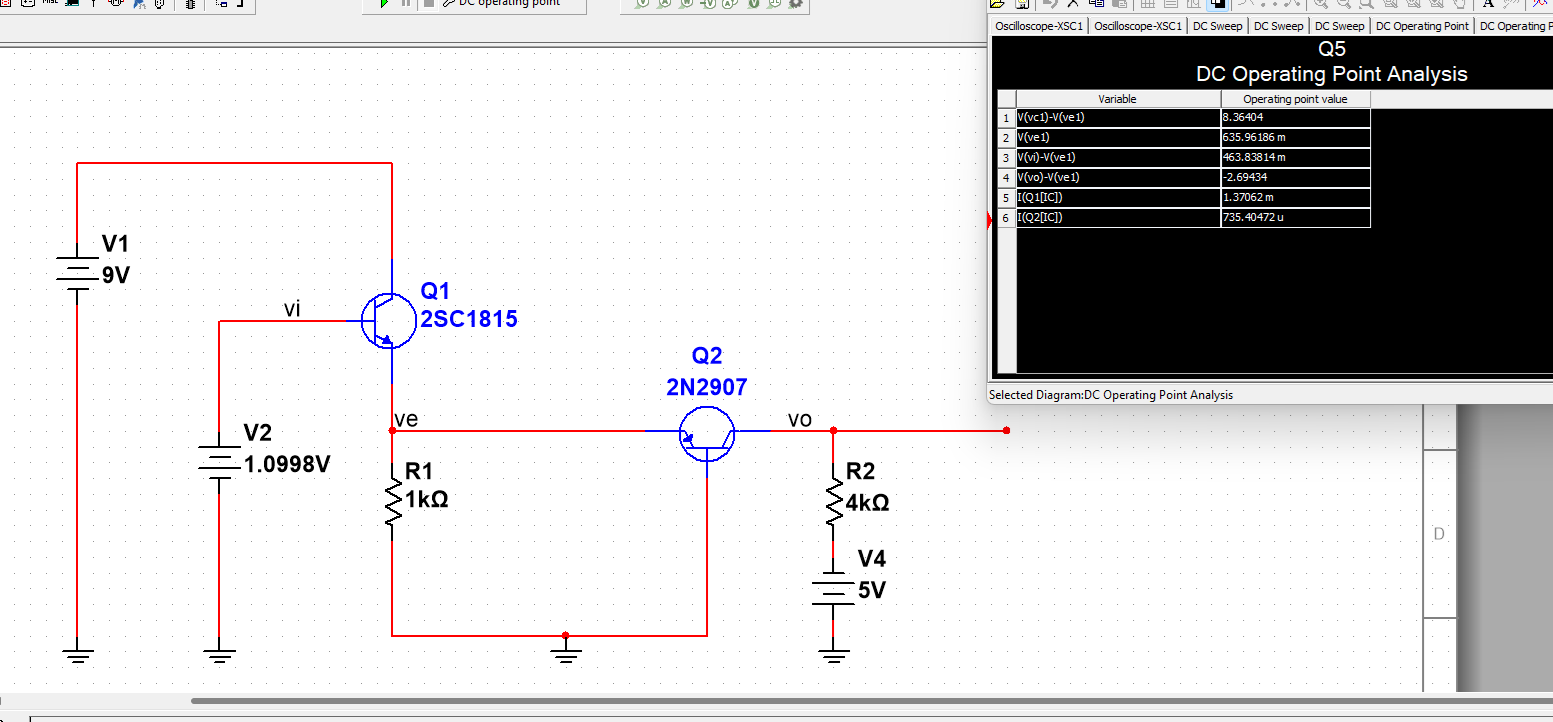
\includegraphics[width=.9\linewidth]{./my-chapters/my-images/Question5/b_Q_tung_mach.png}
	\begin{minipage}{.4\linewidth}
		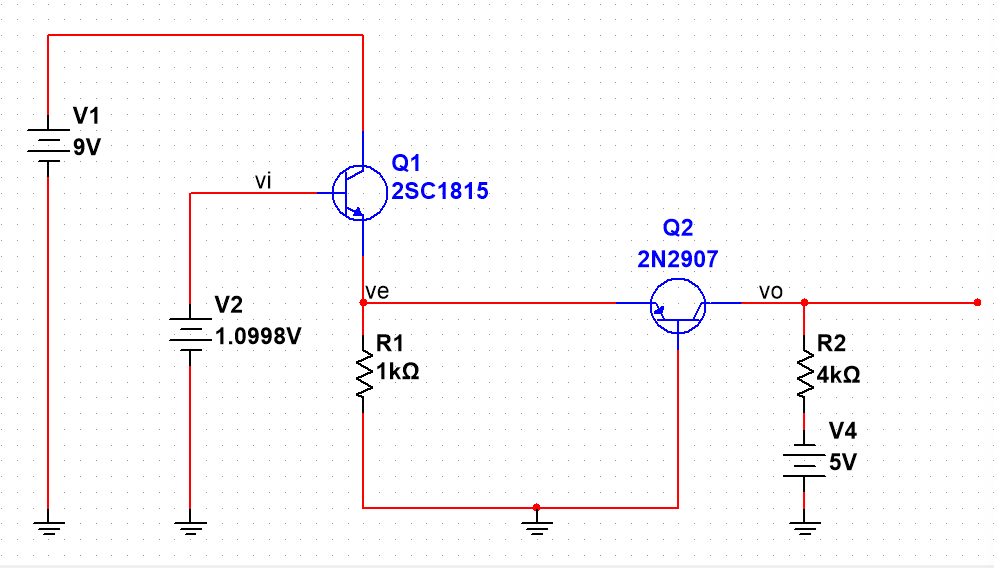
\includegraphics[width=\linewidth]{./my-chapters/my-images/Question5/b_Q_tong_hinh.png}
	\end{minipage}
	\begin{minipage}{.5\linewidth}
		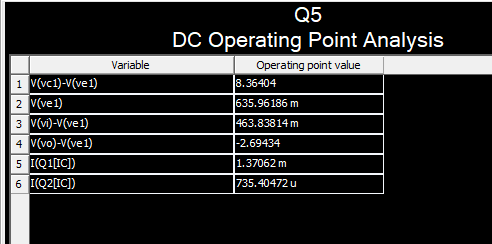
\includegraphics[width=\linewidth]{./my-chapters/my-images/Question5/b_Q_tong_bang.png}
	\end{minipage}
\end{figure}

\begin{itemize}[label=-, leftmargin=2cm]
	\item \finalresult{Q_{1} = (I_{CQ1}, V_{CEQ1}) = (1.3706\,\text{mA}, 8.3640\,\text{V})}
	\item \finalresult{Q_{2} = (I_{CQ2}, V_{CEQ2}) = (0.7354\,\text{mA}, -2.6943\,\text{V})}
\end{itemize}

Ta sử dụng một mạch phân cực $R_{1}$ và $R_{2}$ như sau:

\begin{figure}[H]
	\centering
	\begin{minipage}{.4\linewidth}
		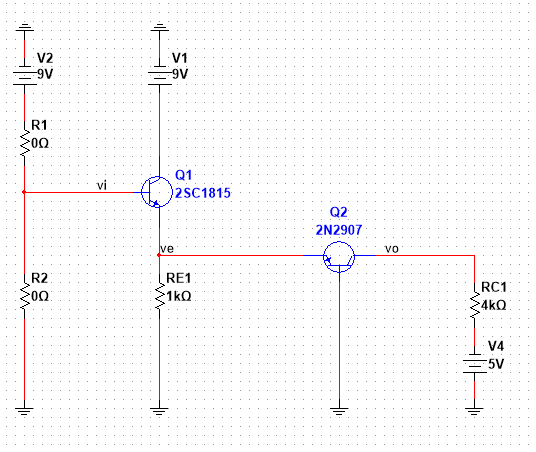
\includegraphics[width=\linewidth]{./my-chapters/my-images/Question5/b_phancuc_R1_R2.png}
	\end{minipage}
	\begin{minipage}{.1\linewidth}
		$\Rightarrow$
	\end{minipage}
	\begin{minipage}{.4\linewidth}
		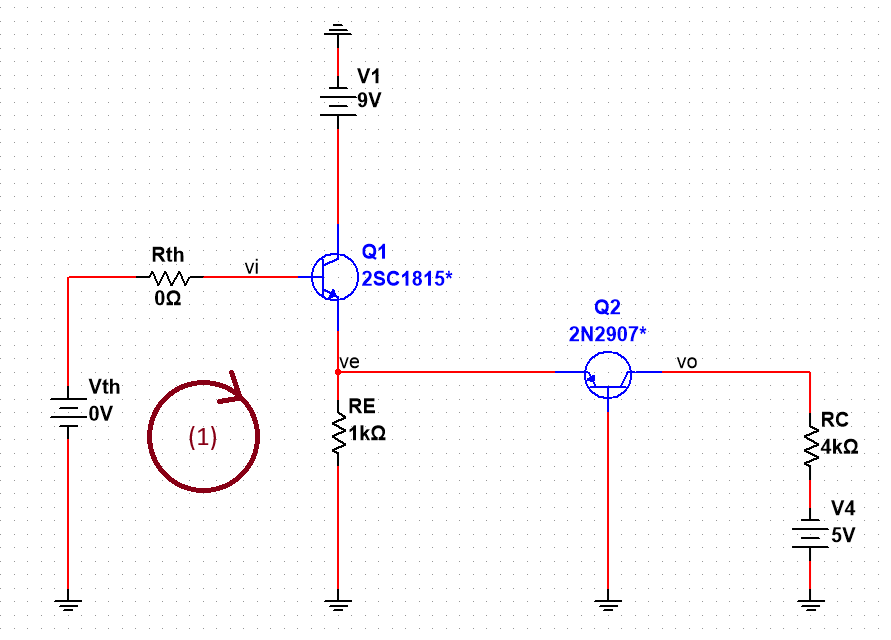
\includegraphics[width=\linewidth]{./my-chapters/my-images/Question5/b_phancuc_thevenin.png}
	\end{minipage}
\end{figure}

Ta có, $I_{C1} = 1.3706\,\text{mA} \Rightarrow I_{B1} = \dfrac{I_{C1}}{\beta} = \dfrac{1.3706}{100} = 0.013706\,\text{mA}$.

$I_{RE} = I_{E1} - I_{E2} = \dfrac{I_{C1}}{\alpha} - \dfrac{I_{C2}}{\alpha} = \dfrac{1.3706}{\dfrac{100}{100+1}} - \dfrac{0.7354}{\dfrac{100}{100+1}} = 0.64582\,\text{mA}$

Viết KCL cho vòng (1):

\[ V_{th} = R_{th}I_{B1} + V_{BE1} + I_{RE}R_{E} \]
\[ \Leftrightarrow 9\times \dfrac{R_{2}}{R_{1} + R_{2}} = \dfrac{R_{1}R_{2}}{R_{1} + R_{2}}\times I_{B1} + V_{BE1} + R_{E}I_{RE} \]
\[ \Leftrightarrow \dfrac{R_{2}}{R_{1} + R_{2}}\left( 9 - R_{1}\times 0.013706 \right) = 1.1097 \]

Với chọn $R_{2} = 22\,\text{k}\Omega \Rightarrow R_{1} = 123.0036\,\text{k}\Omega$.

Kết quả mô phỏng,

\begin{figure}[H]
	\centering
	\begin{minipage}{.4\linewidth}
		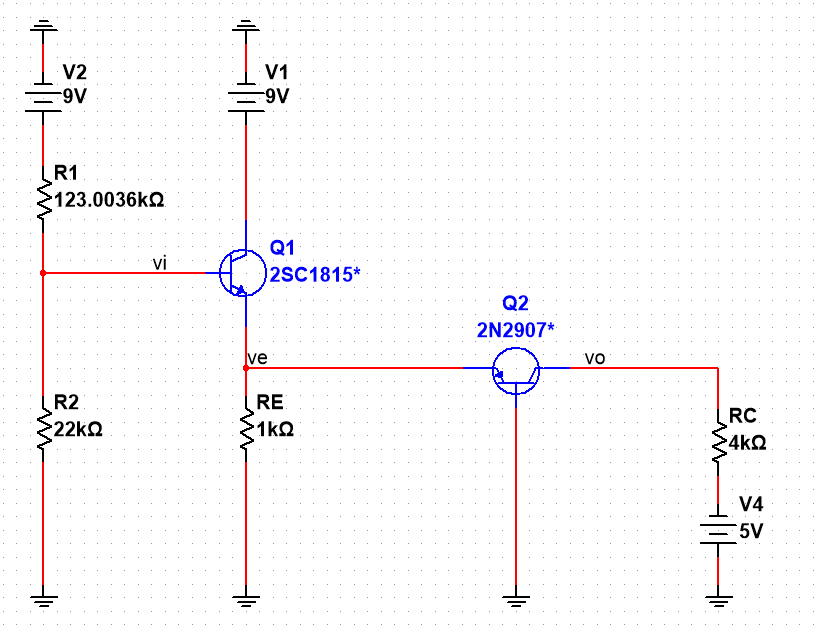
\includegraphics[width=\linewidth]{./my-chapters/my-images/Question5/b_ketqua_R1R2.png}
	\end{minipage}
	\begin{minipage}{.4\linewidth}
		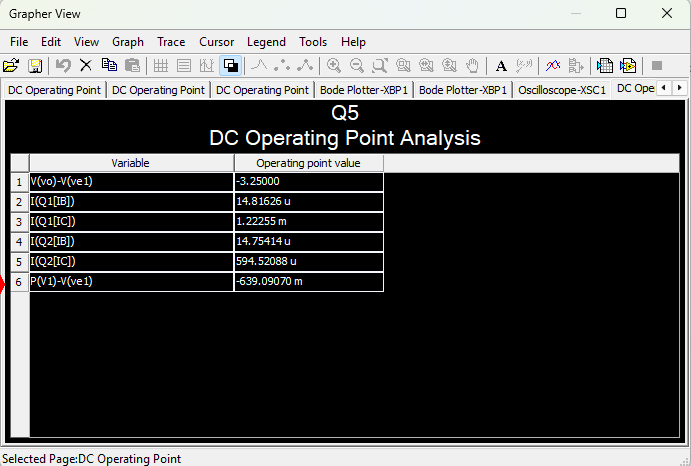
\includegraphics[width=\linewidth]{./my-chapters/my-images/Question5/b_ketqua.png}
	\end{minipage}
\end{figure}

\answer{c}{Lựa chọn tụ $C_{1}$ (ghép tín hiệu) và $C_{2}$ (ghép tải) để mạch có $f_{L}=200Hz$. Giả sử tín hiệu có nội trở $100\Omega$ và tải có điện trở $100\Omega$. Sử dụng phần mềm mô phỏng, vẽ đáp ứng tần số của mạch.}

\begin{figure}[H]
	\centering
	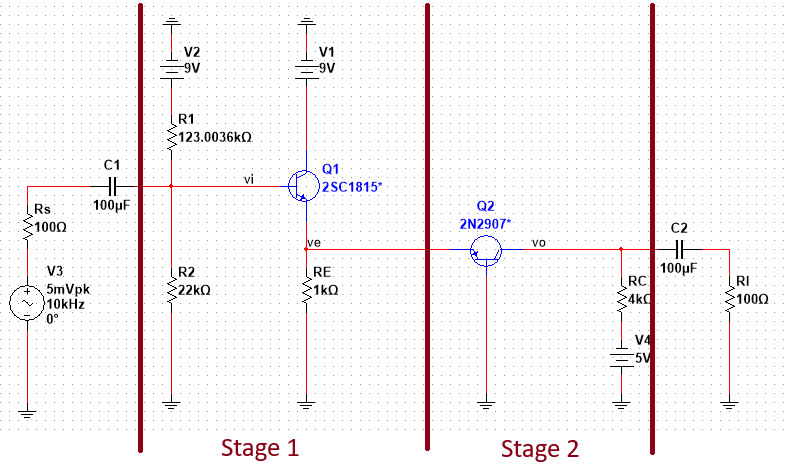
\includegraphics[width=.8\linewidth]{./my-chapters/my-images/Question5/c_machtongquan.png}
\end{figure}

\begin{itemize}[label=-]
	\item Với tầng 1
	
	\begin{figure}[H]
		\centering
		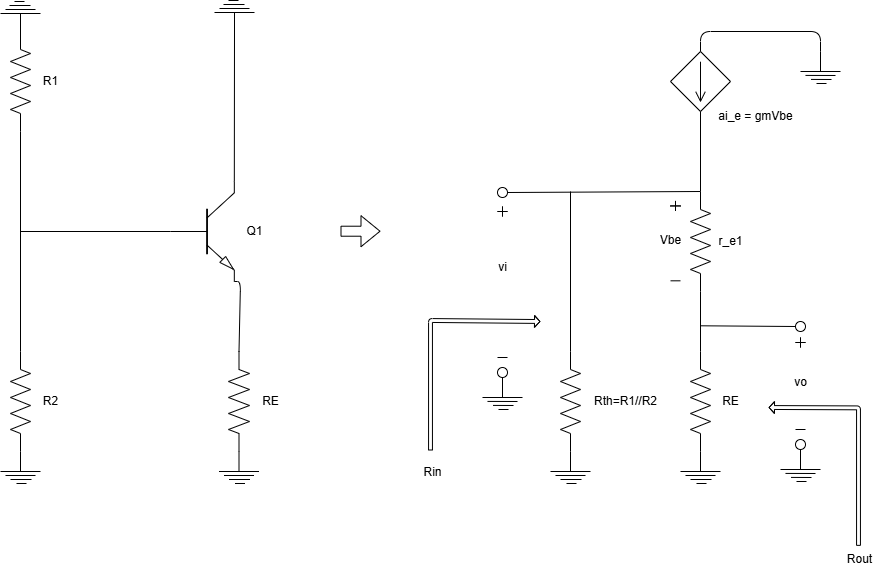
\includegraphics[width=.8\linewidth]{./my-chapters/my-diagrams/Question5/cauc_stage1.png}
	\end{figure}
	
	\begin{itemize}[label=+, leftmargin=2cm]
		\item $r_{e1} = \dfrac{V_{T}}{I_{E1}} = 18.0560\,\Omega$
		\item $r_{\pi1} = \beta\dfrac{V_{T}}{I_{C1}} = 1.8240\,\text{k}\Omega$
		\item $g_{m1} = \dfrac{I_{C1}}{V_{T}} = 54.824\,\text{mS}$
	\end{itemize}
	
	Tính $R_{in1} = \dfrac{v_{i}}{i_{i}}\bigg|_{i_{o} = 0} = R_{th} // (\beta + 1)(r_{e1} + R_{E})$
	
	$\Rightarrow R_{in1} = 15.7954\,\text{k}\Omega$
	
	Tính $R_{out1} = \dfrac{v_{o}}{i_{o}}\bigg|_{v_{i} = 0} = r_{e1} // R_{E}$
	
	$\Rightarrow R_{out1} = 17.7358\,\Omega$
	
	Tính $A_{vo1} = \dfrac{vo}{vi}\bigg|_{R_{L} = \infty} = \dfrac{R_{E}}{R_{E} + r_{e1}}$
	
	$\Rightarrow A_{vo1} = 0.9823\,\text{V/V}$
	\item Với tầng 2
	
	\begin{figure}[H]
		\centering
		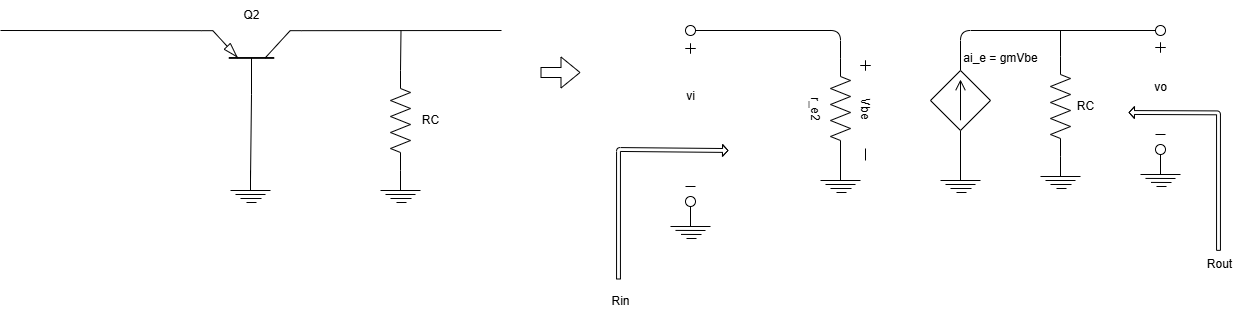
\includegraphics[width=.8\linewidth]{./my-chapters/my-diagrams/Question5/cauc_stagte2.png}
	\end{figure}
	
	\begin{itemize}[label=+, leftmargin=2cm]
		\item $r_{e2} = \dfrac{V_{T}}{I_{E2}} = 33.6585\,\Omega$
		\item $r_{\pi2} = \beta\dfrac{V_{T}}{I_{C2}} = 2.7196\,\text{k}\Omega$
		\item $g_{m2} = \dfrac{I_{C1}}{V_{T}} = 29.416\,\text{mS}$
	\end{itemize}
	
	Tính $R_{in2} = \dfrac{v_{i}}{i_{i}}\bigg|_{i_{o} = 0} = r_{e2}$
	
	$\Rightarrow R_{in2} = 33.6585\,\Omega$
	
	Tính $R_{out2} = \dfrac{v_{o}}{i_{o}}\bigg|_{v_{i} = 0} = R_{C}$
	
	$\Rightarrow R_{out2} = 4\,\text{k}\Omega$
	
	Tính $A_{vo2} = \dfrac{vo}{vi}\bigg|_{R_{L} = \infty} = g_{m2} R_{C}$
	
	$\Rightarrow A_{vo2} = 117.664\,\text{V/V}$
\end{itemize}

Sau khi tính các giá trị của các tầng, ta có mô hình tổng quát như sau

\begin{figure}[H]
	\centering
	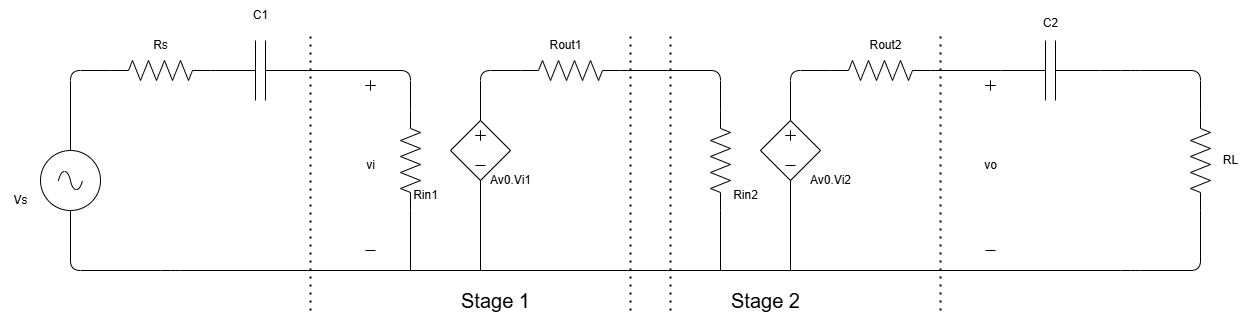
\includegraphics[width=\linewidth]{./my-chapters/my-diagrams/Question5/c_tonghopmach.png}
\end{figure}

\begin{itemize}[label=-]
	\item Xét tụ $C_{1}$:
	\[ \tau_1 = C_{1} \left( R_{s} + R_{in1} \right) \Rightarrow f_{1} = \dfrac{1}{2\pi \tau_1} \]
	\[ \Rightarrow C_{1} = \dfrac{1}{2\pi f_{1} \left( R_{s} + R_{in1} \right)} \]
	
	\item Xét tụ $C_{2}$:
	\[ \tau_{2} = C_{2} \left( R_{out2} + R_{L}\right) \Rightarrow f_{2} = \dfrac{1}{2\pi \tau_{2}}\]
	\[ \Rightarrow C_{2} = \dfrac{1}{2\pi f_{2} \left( R_{out2} + R_{L}\right)}\]
\end{itemize}

Chọn $f_{1} = 200\,\textsf{Hz} = f_{L}$, và cho $f_{2} = \dfrac{f_{1}}{10} = 20\,\textsf{Hz}$

$\Rightarrow$ \finalresult{C_{1} \approx 50.0632 n\,\textsf{F}}.

$\Rightarrow$ \finalresult{C_{2} \approx 1.9409 \,\mu\textsf{F}}.

\begin{figure}[H]
	\centering
	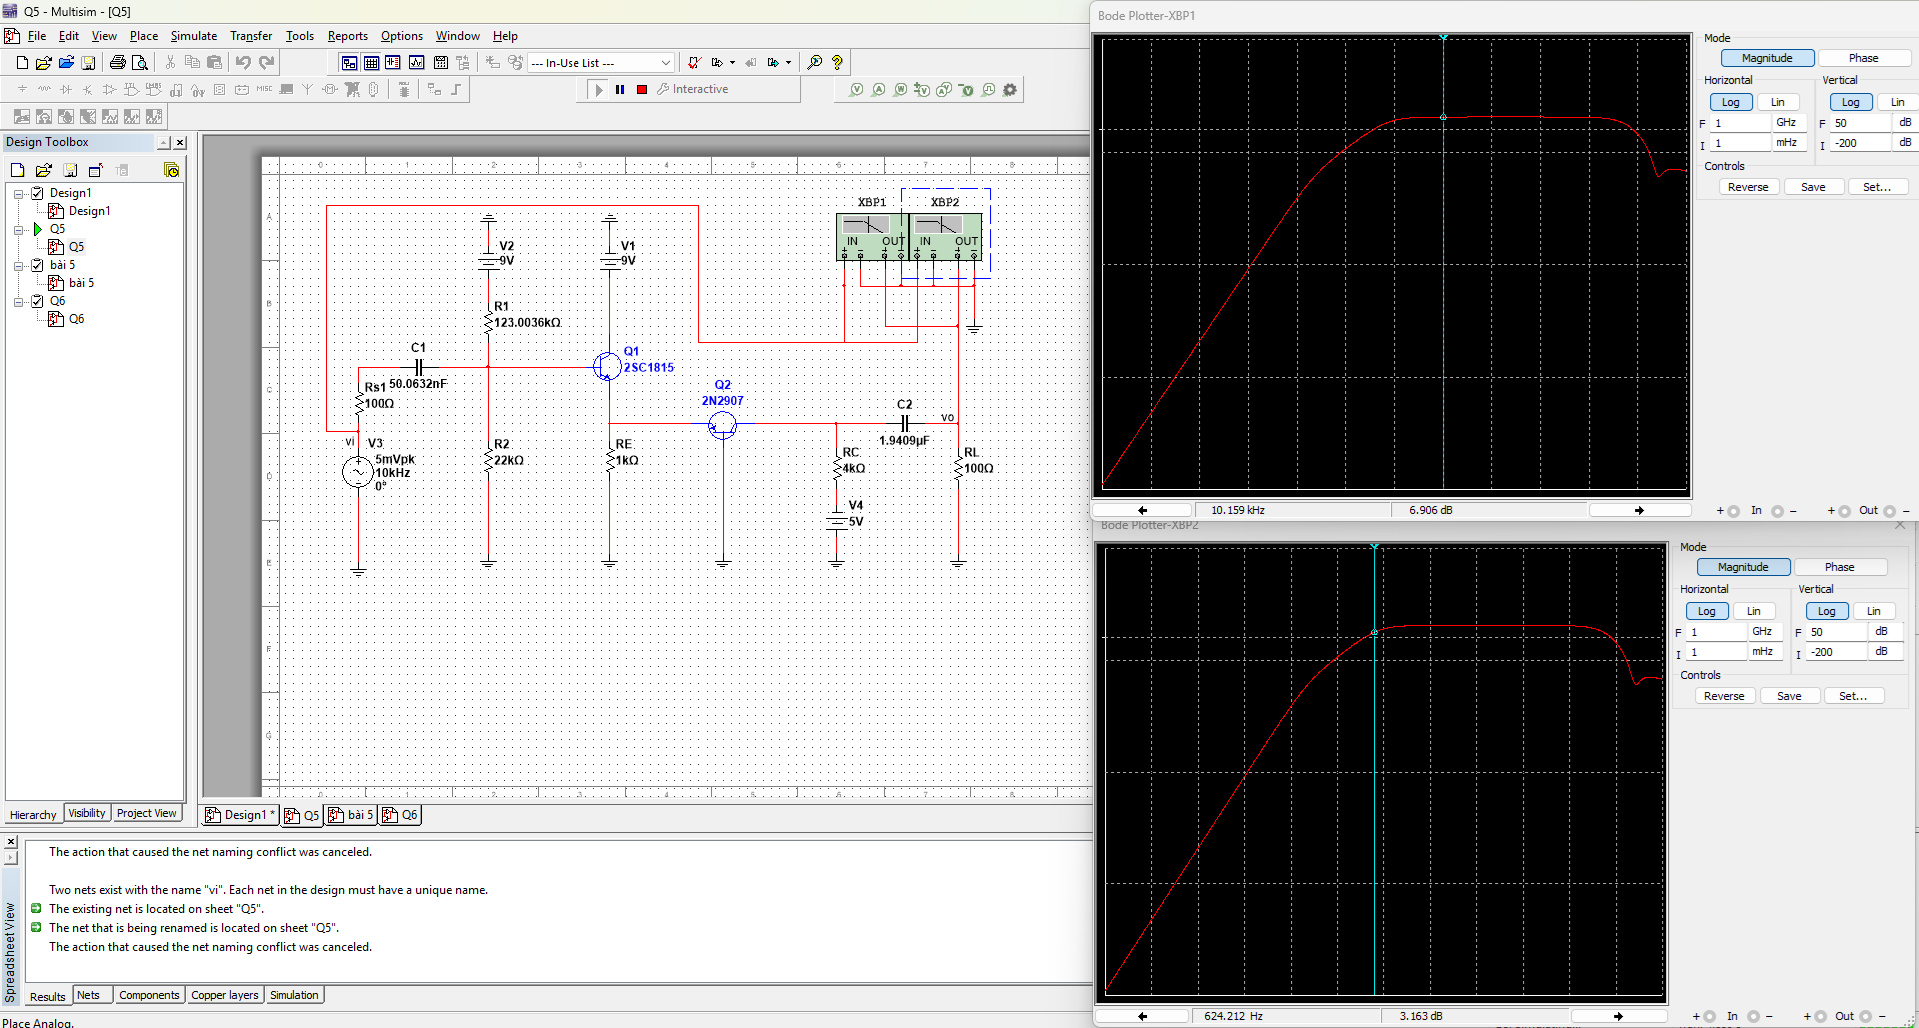
\includegraphics[width=\linewidth]{./my-chapters/my-images/Question5/c_do_bode_socap.png}
	\caption{Ta thấy tại điểm cắt $-3dB$ ta có $f_{L} \approx 624.212\,\textsf{Hz}$.}
\end{figure}

\begin{figure}[H]
	\centering
	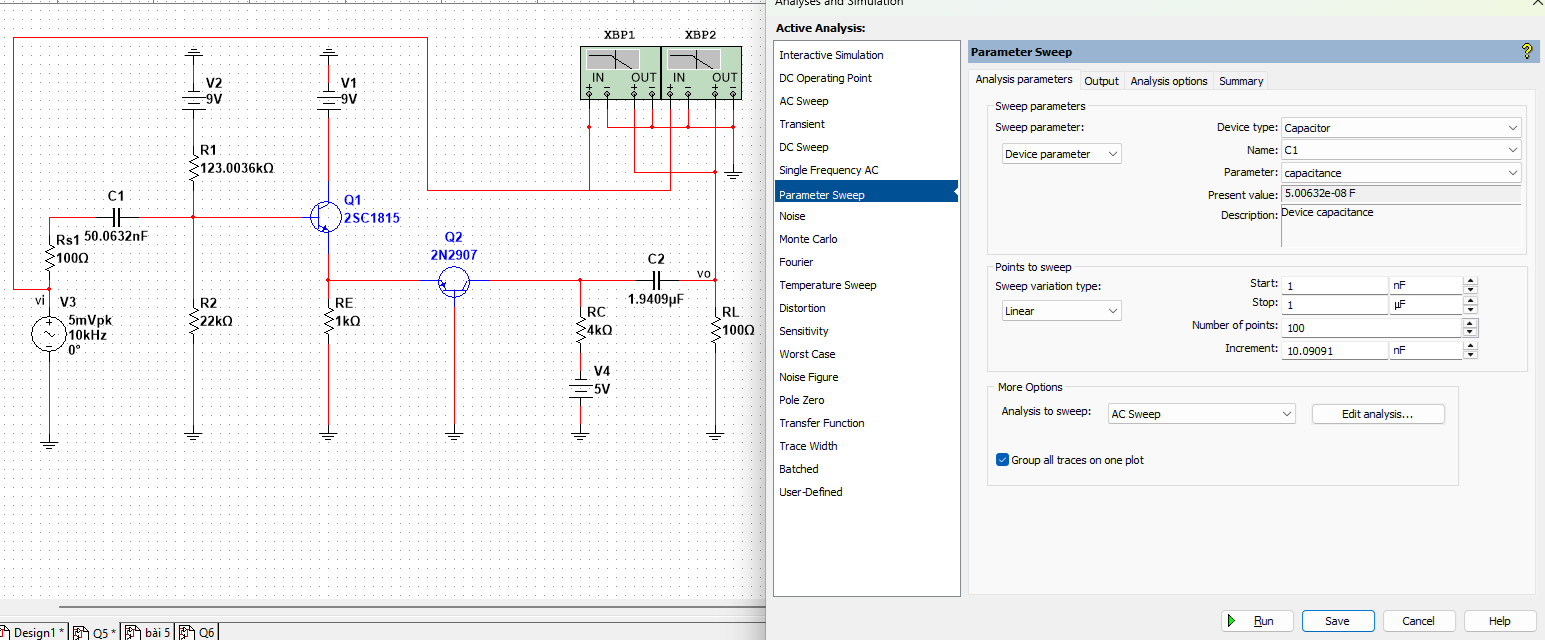
\includegraphics[width=\linewidth]{./my-chapters/my-images/Question5/c_sweep.png}
	\caption{Tiến hành sweep giá trị $C1$ để tìm điểm hợp lý.}
\end{figure}

\begin{figure}[H]
	\centering
	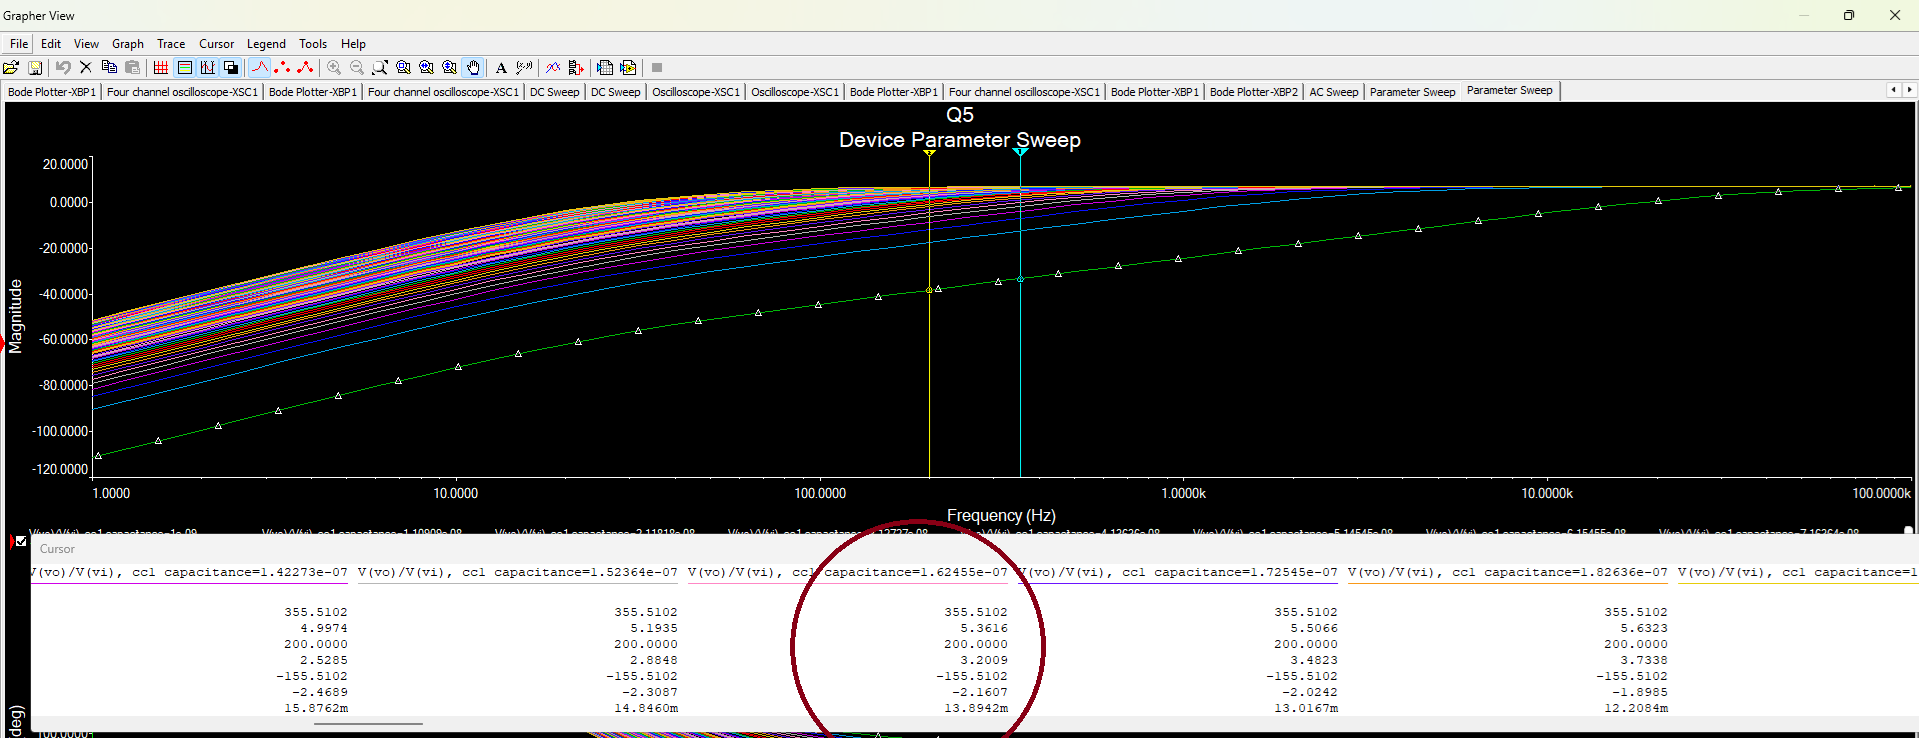
\includegraphics[width=\linewidth]{./my-chapters/my-images/Question5/c_sweep_c.png}
	\caption{Chọn điểm $-3dB$ so với giá trị $G_{v}$ của mạch.}
\end{figure}

Từ ảnh trên ta chọn được \finalresult{C_{1} \approx 162.46 \,\textsf{nF}}.

Tiến hành chạy lại để kiểm tra kết quả cuối cùng

\begin{figure}[H]
	\centering
	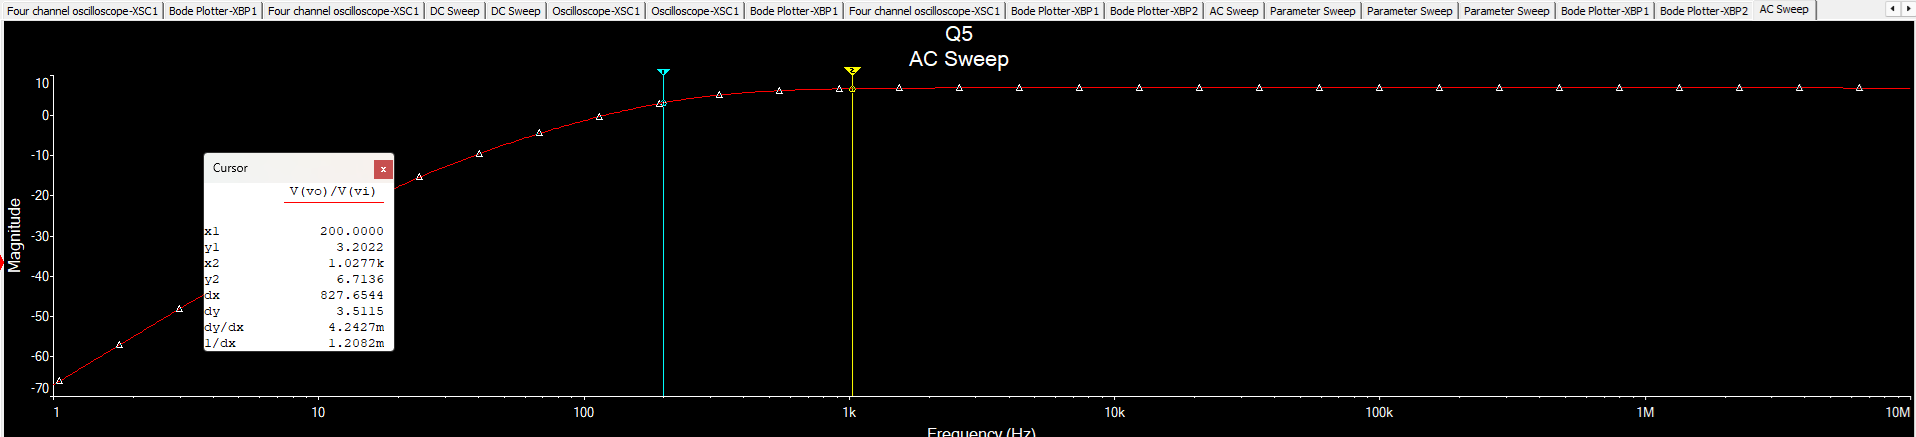
\includegraphics[width=\linewidth]{./my-chapters/my-images/Question5/c_final.png}
	\caption{Sau khi thay đổi $C_{1}$ ta có $f_{L} = 200\,\textsf{Hz}$.}
\end{figure}

\answer{d}{ Đặt vào mạch tín hiệu xoay chiều có biên độ $5\,\text{mV}$ và tần số $10$KHz.  Sử dụng phần mềm mô phỏng, cho biết tín hiệu tại $V_{o1}$ và $V_{o2}$. Giải thích}

\begin{figure}[H]
	\centering
	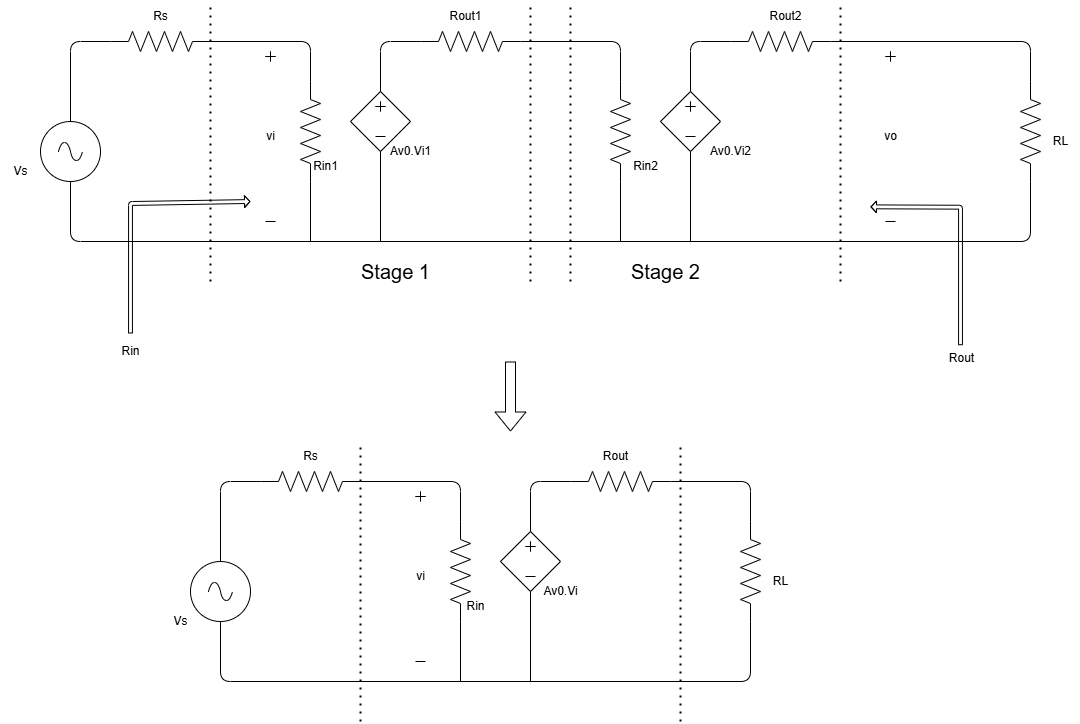
\includegraphics[width=.9\linewidth]{./my-chapters/my-diagrams/Question5/cauc_all_stage.png}
\end{figure}

\begin{itemize}[label=+, leftmargin=2cm]
	\item $A_{vo} = A_{vo2}\dfrac{R_{in2}}{R_{out1} + R_{in2}} A_{vo1} = 75.6951\,\text{V/V}$
	\item $A_{v} = A_{vo} \dfrac{R_{L}}{R_{L} + R_{out2}} = 1.8462\,\text{V/V}$
	\item $G_{v} = \dfrac{R_{s}}{R_{s} + R_{in1}}A_{v} = 1.8346\,\text{V/V} \approx 5.2708dB$
\end{itemize}

\begin{itemize}[label=-]
	\item Tầng 1
	\begin{figure}[H]
		\centering
		\begin{minipage}{.4\linewidth}
			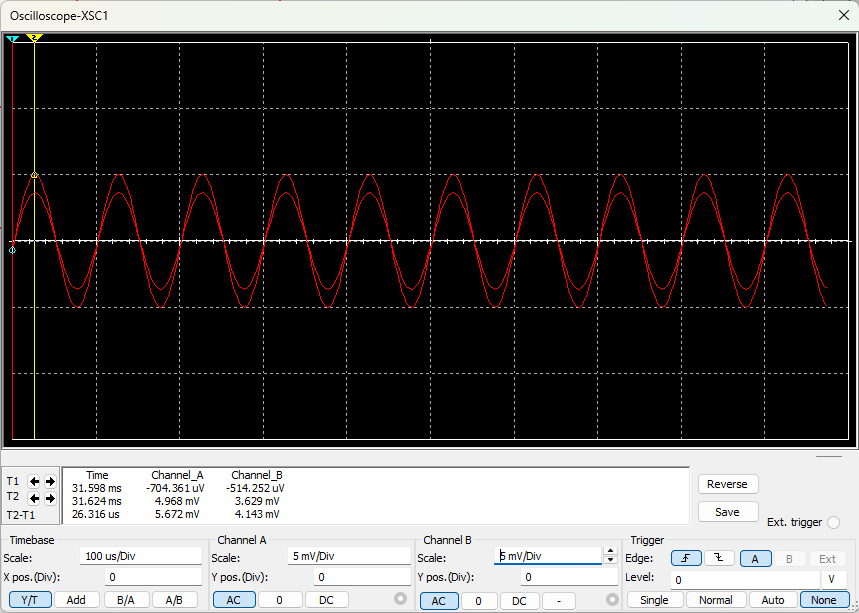
\includegraphics[width=\linewidth]{./my-chapters/my-images/Question5/c_vo1.png}
		\end{minipage}
		\caption{Kết quả khi đo dạng sóng ngỡ ra ở $v_{o1}$.}
	\end{figure}
	
	Vì với $A_{vo1} = 0.9823\,\text{V/V}$ nên tín hiệu ngõ ra có suy giảm một lượng nhỏ so với tín hiệu ngõ vào.
	\item Tầng 2
	\begin{figure}[H]
		\centering
		\begin{minipage}{.4\linewidth}
			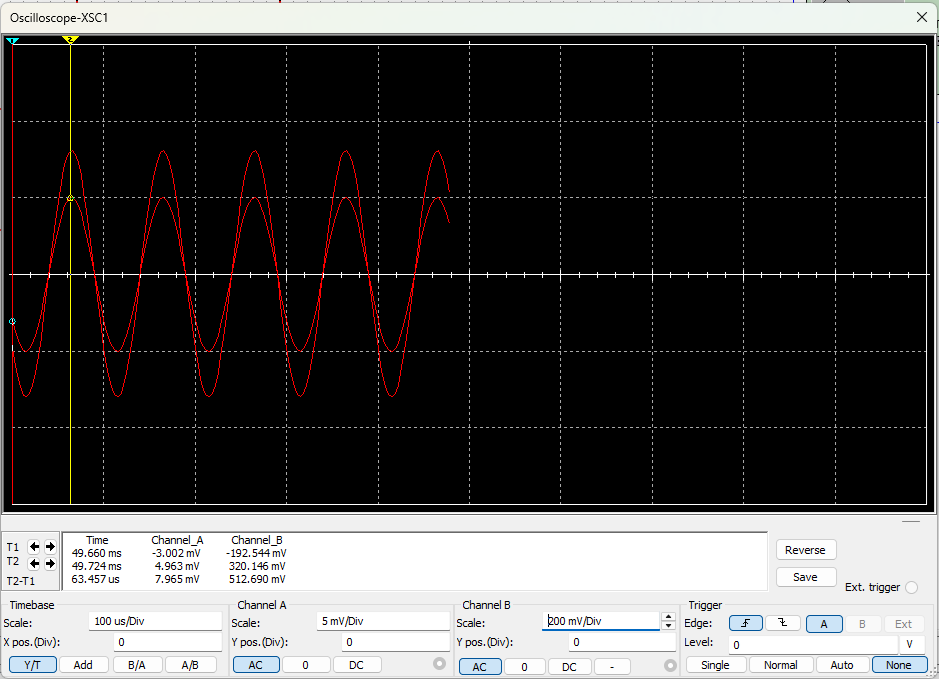
\includegraphics[width=\linewidth]{./my-chapters/my-images/Question5/c_vo2.png}
		\end{minipage}
		\caption{Kết quả khi đo dạng sóng ngỡ ra ở $v_{o2}$.}
	\end{figure}
	
	Vì tới $A_{vo2} = 117.664\,\text{V/V}$ nên tín hiệu ngõ ra ở $v_{o2}$ rất lớn hơn so với tín hiệu ngõ vào.
\end{itemize}

Toàn mạch
\begin{figure}[H]
	\centering
	\begin{minipage}{.4\linewidth}
		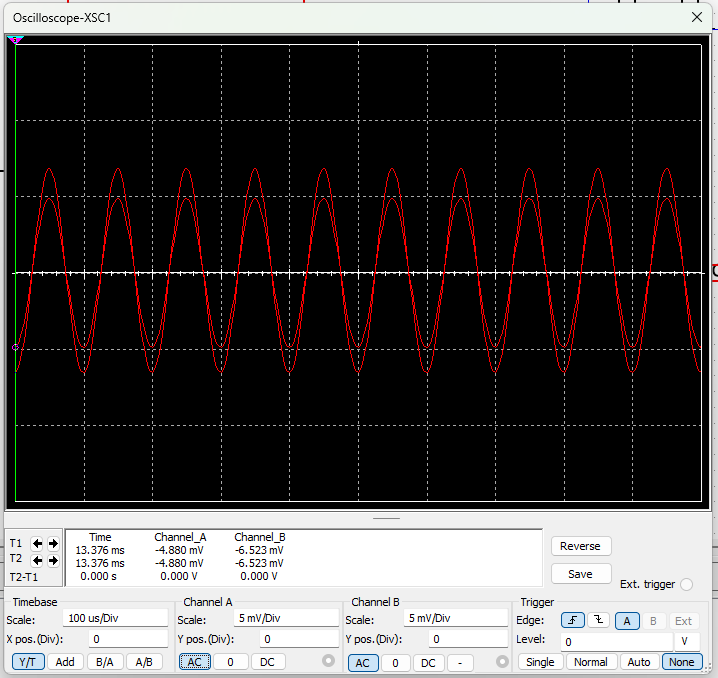
\includegraphics[width=\linewidth]{./my-chapters/my-images/Question5/d_A_Vo.png}
	\end{minipage}
	\begin{minipage}{.4\linewidth}
		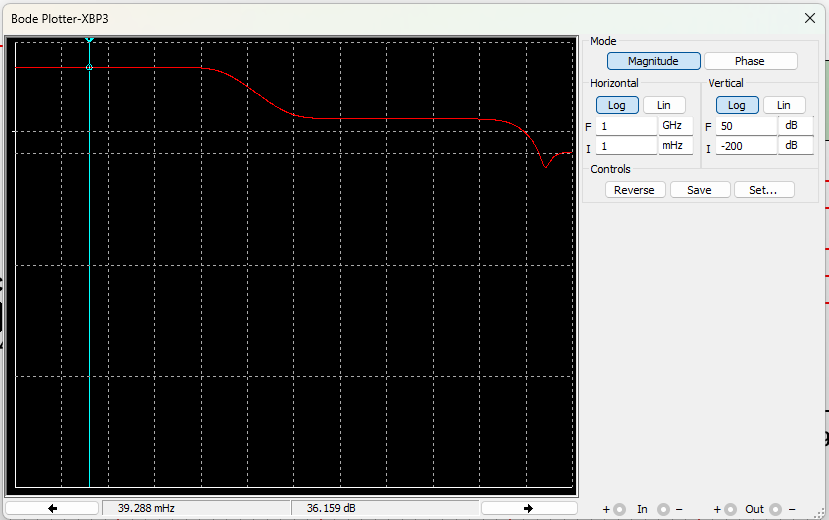
\includegraphics[width=\linewidth]{./my-chapters/my-images/Question5/d_A_vo_ketqua.png}
	\end{minipage}
	\caption{Kết quả khi đo $A_{vo}$ cho toàn mạch.}
\end{figure}
\begin{figure}[H]
	\centering
	\begin{minipage}{.4\linewidth}
		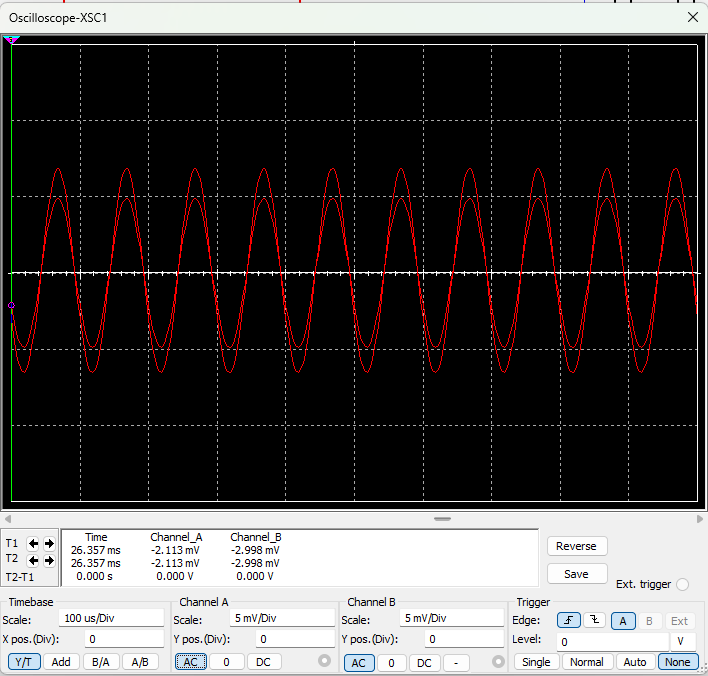
\includegraphics[width=\linewidth]{./my-chapters/my-images/Question5/d_A_V.png}
	\end{minipage}
	\begin{minipage}{.4\linewidth}
		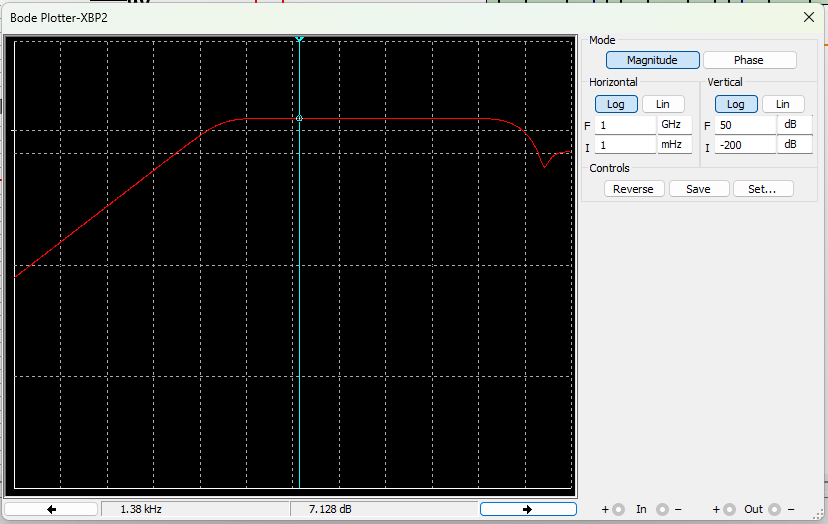
\includegraphics[width=\linewidth]{./my-chapters/my-images/Question5/d_a_v_ketqua.png}
	\end{minipage}
	\caption{Kết quả khi đo $A_{v}$ cho toàn mạch.}
\end{figure}
\begin{figure}[H]
	\centering
	\begin{minipage}{.4\linewidth}
		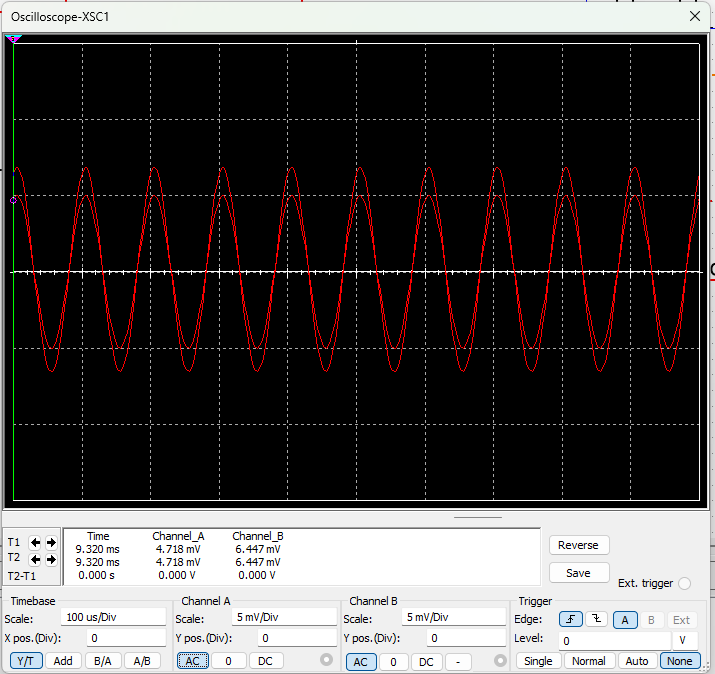
\includegraphics[width=\linewidth]{./my-chapters/my-images/Question5/d_G_V.png}
	\end{minipage}
	\begin{minipage}{.4\linewidth}
		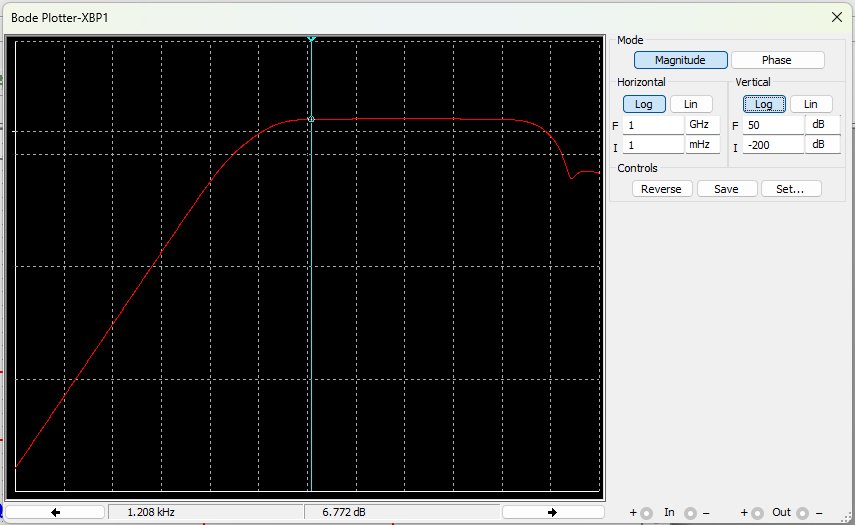
\includegraphics[width=\linewidth]{./my-chapters/my-images/Question5/d_gv_ketqua.png}
	\end{minipage}
	\caption{Kết quả khi đo $G_{v}$ cho toàn mạch.}
\end{figure}
\question{Câu 6}

 Cho mạch khuếch đại tín hiệu được ghép liên tầng như hình vẽ. Giả sử các tụ có điện dung rất lớn. Các thông số $\beta = 100$,  $K_{n}=1 mA/V^{2}$, $V_{TN} = 1 V$. BJT có $V_{A} = \infty$  và FET có $\lambda = 0$. 
 
 \begin{figure}[H]
 	\centering
 	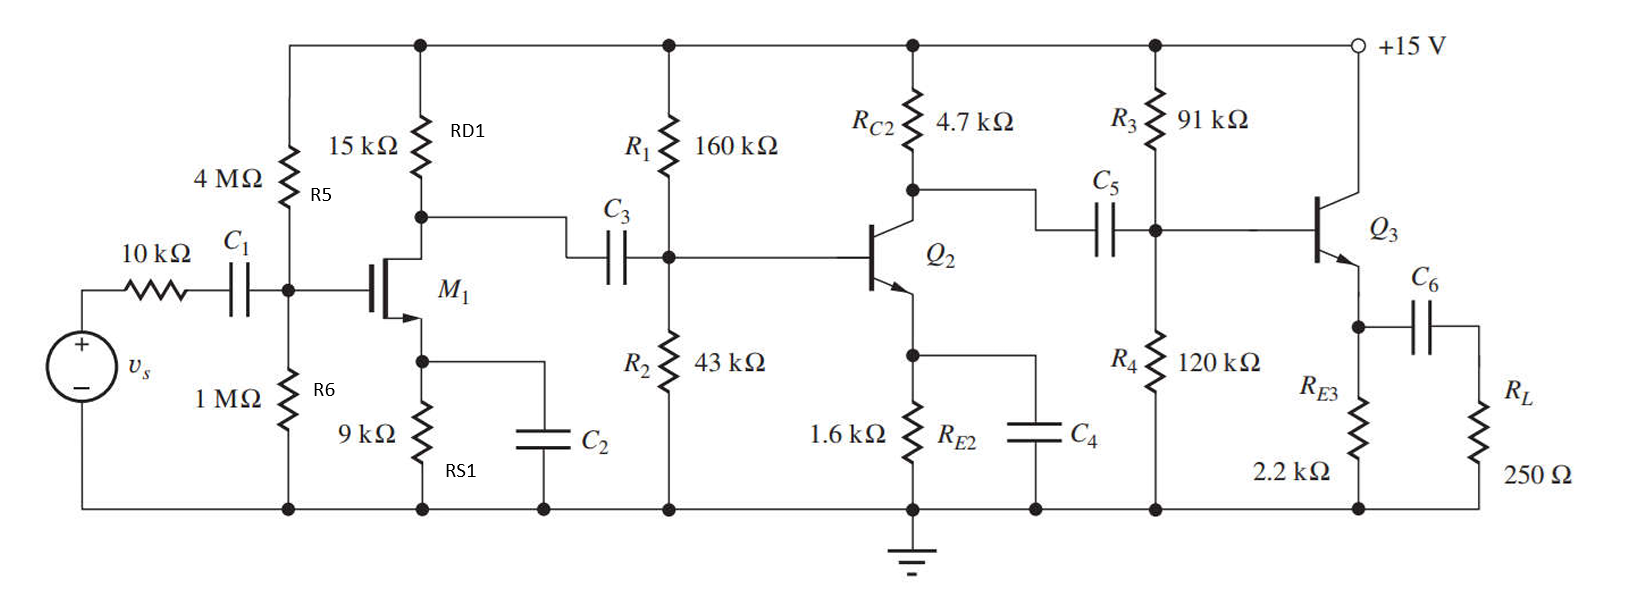
\includegraphics[width=.9\linewidth]{./my-chapters/my-images/Question6/DeBai.png}
 \end{figure}
 
% \begin{enumerate}[label=\alph*)]
% 	\item Tìm điểm hoạt động Q của các transistor.
% \end{enumerate}

\answer{a}{Tìm các điểm hoạt động của Q}

\noindent Xét hoạt động chế độ DC cho toàn mạch.

\begin{itemize}[label=-]

	\item Tầng 1:
	
	\begin{minipage}{0.4\linewidth}
		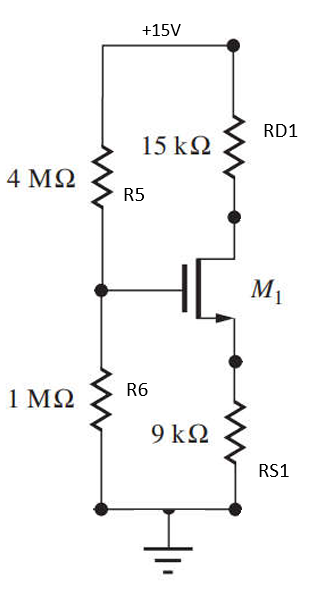
\includegraphics[width=.7\linewidth]{./my-chapters/my-images/Question6/DC_tang1.png}
	\end{minipage}
	\begin{minipage}{0.1\linewidth}
		$\Rightarrow$
	\end{minipage}
	\begin{minipage}{0.4\linewidth}
		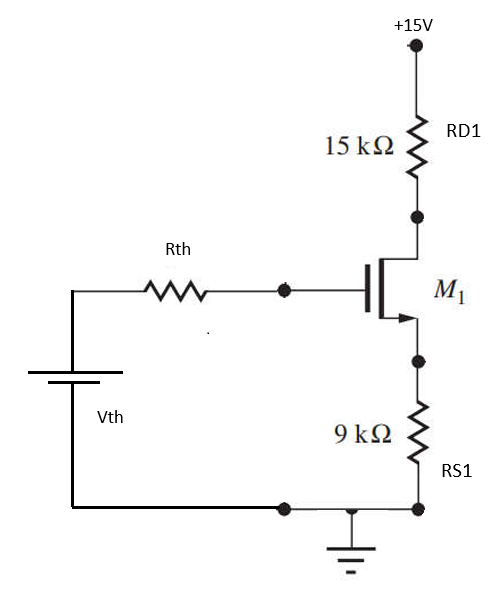
\includegraphics[width=.8\linewidth]{./my-chapters/my-images/Question6/DC_tang1 - Copy.png}
	\end{minipage}
	
	Thevenin ta có:
		\[ R_{th} = R_{5}//R_{6} = \dfrac{4M \times 1M}{4M + 1M} = 0.8M \,\Omega \]
		\[ V_{th} = \dfrac{R6}{R_{5} + R_{6}}\times V_{cc} = \dfrac{1M}{1M + 4M}\times 15 = 3V\]
		$\Rightarrow V_{G} = 3V \Rightarrow V_{GS} = V_{G} - V_{S} = 3 - V_{S}$
		
		Với $V_{S} = I_{DS} \times R_{S1} \Rightarrow V_{GS} = 3 - I_{DS}\times R_{S1}$
		\[ \begin{matrix}
			I_{DS1} & = & \dfrac{1}{2} K_{n} (V_{GS} - V_{tn})^{2} \hfill \\
			       & = & \dfrac{1}{2} K_{n} (3 - I_{DS}\times R_{S1} - V_{tn})^{2} \hfill \\
			       & = & \dfrac{1}{2} (3 - I_{DS}\times 9 - 1)^{2} \hfill \\ 
		\end{matrix}
		\]
		
		\[ \Rightarrow
		\begin{cases}
			I_{DS1} = 0.3097mA \rightarrow V_{GS} = 3 - 0.3097\times 9 = 0.2127V < V_{tn}(\text{Loại}) \\
			I_{DS1} = 0.1595mA \rightarrow V_{GS} = 3 - 0.1595\times 9 = 1.5645V > V_{tn}(\text{Thỏa})
		\end{cases}\]
		$ \Rightarrow V_{D} = V_{cc} - I_{D} \times R_{D1} = 15 - 0.1595\times 15 = 12.6075V $
		
		$ \Rightarrow V_{DS1} = V_{D} - V_{S} = 11.1720V $
		
		Vậy điểm làm việc Q của tâng 1 là : \finalresult{(I_{DS1}, V_{DS1}) = (0.1595mA, 11.1720V)}.
		
		\item Tầng 2:
		
		\begin{minipage}{0.4\linewidth}
			\includegraphics[width=.7\linewidth]{./my-chapters/my-images/Question6/DC_tang2.png}
		\end{minipage}
		\begin{minipage}{0.1\linewidth}
			$\Rightarrow$
		\end{minipage}
		\begin{minipage}{0.4\linewidth}
			\includegraphics[width=.8\linewidth]{./my-chapters/my-images/Question6/DC_tang2 - Copy.png}
		\end{minipage}
		
			Thevenin ta có:
		\[ R_{th} = R_{1}//R_{2} = \dfrac{160k \times 43k}{160k + 43k} \approx 33.8916k \,\Omega \]
		\[ V_{th} = \dfrac{R2}{R_{1} + R_{2}}\times V_{cc} = \dfrac{43k}{160k + 43k}\times 15 \approx 3.1773V\]
		
		Áp dụng KVL cho vòng (1):
		\[ -I_{E2}\times R_{E2} - V_{BE} - I_{B2}\times R_{th} + V_{th} = 0 \]
		Ta có: $I_{E2} = (\beta + 1) I_{B}$
		\[ \Rightarrow I_{B} = \dfrac{V_{th} - V_{BE}}{R_{th} + (\beta + 1)R_{E2}} = \dfrac{3.1773 - 0.7}{33.8916 + (100+1)1.6} = 0.0127mA\]
		Ta có: $I_{C2} = \beta I_{B2} = 100\times 0.0127mA = 1.270mA$.
		
		Áp dụng KVL cho vòng (2):
		\[-V_{cc} + I_{C2}R_{C2} + V_{CE} + I_{E2}R_{E2} = 0 \]
		Ta có: $I_{C2} = \dfrac{\beta}{\beta + 1}I_{E2} = \alpha I_{E2} \approx I_{E2}$
		
		\[ \Rightarrow V_{CE2} = V_{cc} - I_{C2}(R_{C2} + R_{E2}) = 15 - 1.270(4.7 + 1.6) = 6.9990V\]
		
		Vậy điểm làm việc Q của tâng 2 là : \finalresult{(I_{CQ2}, V_{CEQ2}) = (1.270mA, 6.9990V)}.
		
		\item Tầng 3:
		
		\begin{minipage}{0.4\linewidth}
			\includegraphics[width=.7\linewidth]{./my-chapters/my-images/Question6/DC_tang3.png}
		\end{minipage}
		\begin{minipage}{0.1\linewidth}
			$\Rightarrow$
		\end{minipage}
		\begin{minipage}{0.4\linewidth}
			\includegraphics[width=.8\linewidth]{./my-chapters/my-images/Question6/DC_tang3 - Copy.png}
		\end{minipage}
		
		Thevenin ta có:
		\[ R_{th} = R_{3}//R_{4} = \dfrac{91k \times 120k}{91k + 120k} \approx 51.7536k \,\Omega \]
		\[ V_{th} = \dfrac{R4}{R_{3} + R_{4}}\times V_{cc} = \dfrac{120k}{91k + 120k}\times 15 \approx 8.5308V\]
		
		Áp dụng KVL cho vòng (1):
		\[ -I_{E3}\times R_{E3} - V_{BE} - I_{B3}\times R_{th} + V_{th} = 0 \]
		Ta có: $I_{E3} = (\beta + 1) I_{B3}$
		\[ \Rightarrow I_{B3} = \dfrac{V_{th} - V_{BE}}{R_{th} + (\beta + 1)R_{E3}} = \dfrac{8.5308 - 0.7}{51.7536 + (100+1)2.2} = 0.0286mA\]
		Ta có: $I_{C3} = \beta I_{B3} = 100\times 0.0286mA = 2.86mA$.
		
		Áp dụng KVL cho vòng (2):
		\[-V_{cc} + V_{CE} + I_{E}R_{E2} = 0 \]
		Ta có: $I_{C3} = \dfrac{\beta}{\beta + 1}I_{E3} = \alpha I_{E3} \approx I_{E}$
		
		\[ \Rightarrow V_{CE3} = V_{cc} + R_{E2}I_{E3} = 15 - 2.86(2.2) = 8.708V\]
		
		Vậy điểm làm việc Q của tâng 3 là : \finalresult{(I_{CQ3}, V_{CEQ3}) = (2.86mA, 8.708V)}.
\end{itemize}

Kiểm chứng kết quả

\begin{figure}[H]
	\centering
	\begin{minipage}{.4\linewidth}
		\includegraphics[width=\linewidth]{./my-chapters/my-images/Question6/a_machdophancuc.png}
	\end{minipage}
	\begin{minipage}{.4\linewidth}
	\includegraphics[width=\linewidth]{./my-chapters/my-images/Question6/a_dophancuc.png}
	\end{minipage}
\end{figure}

\answer{b}{Tìm $A_{v}$, $G_{v}$, $R_{i}$, $R_{o}$ của mạch.}

\noindent Xét hoạt động chế độ AC cho toàn mạch, ta có mạch tương đương như sau:

\begin{figure}[H]
	\centering
	\includegraphics[width=.9\linewidth]{./my-chapters/my-diagrams/Question6/caub_tongquat.png}
\end{figure}

\begin{itemize}[label=-]
	\item Tầng 1:
	
	\begin{figure}[H]
		\centering
		\includegraphics[width=.7\linewidth]{./my-chapters/my-diagrams/Question6/caub_stage1.png}
	\end{figure}
	
	\begin{itemize}[label = +]
		\item $R_{in1} = \dfrac{v_{i}}{i_{i}}|_{v_{o}=0} = R_{5} // R_{6} = \dfrac{4M \times 1M}{4M + 1M} = 0.8M \,\Omega$
		\item $R_{out1} = \dfrac{v_{o}}{i_{o}}|_{i_{i} = 0} = R_{D1} = 15k \,\Omega$
		\item $A_{vo_{1}} = \dfrac{v_{o_{1}}}{v_{i_{1}}}|_{R_{L} = \infty} = \dfrac{v_{o_{1}}}{V_{gs}} = -g_{m} R_{D1}$
		
		Trong đó, $g_{m} = \dfrac{2I_{DQ}}{V_{OV}} = \dfrac{2I_{DQ}}{V_{GS} - V_{tn}} = \dfrac{2\times 0.1595mA}{1.5645V - 1V} \approx 0.5651 mA/V$
		
		$\Rightarrow A_{vo_{1}} = -0.5651 mA/V \times 15k = -8.4765 V/V $.
	\end{itemize}
	
	\item Tầng 2:
	
	\begin{figure}[H]
		\centering
		\includegraphics[width=.7\linewidth]{./my-chapters/my-diagrams/Question6/caub_stage2.png}
	\end{figure}
	
	\begin{itemize}[label = +]
		\item $R_{in2} = \dfrac{v_{i}}{i_{i}}|_{i_{o}=0} = R_{1} // R_{2} // r_{\pi}$
		
		Trong đó, $r_{\pi} = \dfrac{\beta}{g_{m}} = \beta \dfrac{V_{T}}{I_{C}} = 100 \dfrac{25mV}{1.270mA} = 1.9685k\,\Omega$
		
		$\Rightarrow R_{in2} = 1.8604k\,\Omega$
		\item $R_{out2} = \dfrac{v_{o}}{i_{o}}|_{v_{i} = 0} = R_{C2} = 4.7k \,\Omega$
		\item $A_{vo_{2}} = \dfrac{v_{o_{2}}}{v_{i_{2}}}|_{R_{L} = \infty} = \dfrac{v_{o_{2}}}{v_{be}} = -g_{m}R_{C2}$
		
		Trong đó, $g_{m} = \dfrac{I_{C}}{V_{T}} = \dfrac{1.270mA}{25mV} = 0.0508 A/V$
		
		$\Rightarrow A_{v_{o_{2}}} = -0.0508\times 4.7k = -238.76 V/V$.
	\end{itemize}
	
	\item Tầng 3:
	
	\begin{figure}[H]
		\centering
		\includegraphics[width=.7\linewidth]{./my-chapters/my-diagrams/Question6/caub_stage3.png}
	\end{figure}
	
	\begin{itemize}[label = +]
		\item $R_{in3} = \dfrac{v_{i}}{i_{i}}|_{i_{o}=0} = R_{3} // R_{4} // ((\beta + 1)(r_{e} + R_{E3}))$
		
		Trong đó, $r_{e} = \alpha\dfrac{V_{T}}{I_{C}} = \dfrac{\beta}{\beta + 1}\dfrac{V_{T}}{I_{C}} = \dfrac{100}{100+1} \dfrac{25mV}{2.86mA} = 8.6547\,\Omega$
		
		$\Rightarrow R_{in3} = 42.0078k\,\Omega$
		\item $R_{out3} = \dfrac{v_{o}}{i_{o}}|_{v_{i} = 0} = (r_{e} // R_{E3}) = 8.6208\,\Omega$
		\item $A_{vo_{3}} = \dfrac{v_{o_{3}}}{v_{i_{3}}}|_{R_{L} = \infty} = \dfrac{R_{E3}}{r_{e} + R_{E3}} = 0.9961 V/V$
		
		$\Rightarrow A_{v_{o_{3}}} = 0.9961 V/V$.
	\end{itemize}
\end{itemize}

\noindent Cuối cùng ta có mạch tương đương như sau:

\begin{figure}[H]
	\centering
	\includegraphics[width=.9\linewidth]{./my-chapters/my-diagrams/Question6/caub_1.png}
\end{figure}

\begin{itemize}[label =-]
	\item \finalresult{R_{in} = R_{in1} = 0.8M \,\Omega}
	\item \finalresult{R_{out} = R_{out3} = 8.6208 \,\Omega}
	\item $A_{vo} = \dfrac{v_{o}}{v_{i}}|_{R_{L} = \infty}$
	
	$\begin{matrix}
			   & = & A_{vo_{3}} \dfrac{R_{in3}}{R_{in3} + R_{out2}} A_{vo_{2}} \dfrac{R_{in2}}{R_{in2} + R_{out1}}A_{vo_{1}} \hfill\\
			   & = & 200.0600 \, V/V \hfill
	\end{matrix}$
	
	$\Rightarrow$ \finalresult{A_{vo} = 200.0600 \, V/V}

	\item $A_{v} = A_{vo} \dfrac{R_{L}}{R_{L} + R_{out3}} = 193.3913\, V/V$
	
	$\Rightarrow$ \finalresult{A_{v} = 193.3913\, V/V}
	\item $G_{v} = \dfrac{R_{in1}}{R_{in1} + R_{s}} A_{v} = 191.0038\, V/V$
	
	$\Rightarrow$ \finalresult{G_{v} = 191.0038 \, V/V}
\end{itemize}

Kiểm tra kết quả

\begin{figure}[H]
	\centering
	\includegraphics[width=.8\linewidth]{./my-chapters/my-images/Question6/b_bode_A_vo.png}
	\caption{Với $A_{vo} = 47.94db = 249.44595\,\text{V/V}$.}
\end{figure}

\begin{figure}[H]
	\centering
	\includegraphics[width=.8\linewidth]{./my-chapters/my-images/Question6/b_bode_A_v.png}
	\caption{Với $A_{v} = 46.335db = 207.3719\,\text{V/V}$.}
\end{figure}

\begin{figure}[H]
	\centering
	\includegraphics[width=.8\linewidth]{./my-chapters/my-images/Question6/b_bode_G_v.png}
	\caption{Với $G_{v} = 46.121db = 202.3252\,\text{V/V}$.}
\end{figure}

\answer{c}{Vẽ dạng sóng ngõ vs và vo khi đi qua từng tầng (vị trí trước khi đi qua tụ ghép).}

\noindent Cho $V_{s} = 5\sin\left(\,\Omega t\right) (mV)$

\begin{itemize}[label=-]
	\item Qua tầng đầu tiên, Tầng 1
	
	\begin{figure}[H]
		\centering
		\includegraphics[width=.8\linewidth]{./my-chapters/my-images/Question6/c_stage_1.png}
	\end{figure}
	
	Ta thấy với $A_{vo1} = -8.4765\,\text{V/V}$ với tính toán thì sóng bị đảo pha so với sóng ban đầu và được khuếch đại lên $8.4765$ lần.
	
	\item Qua tấng tiếp theo, Tầng 2
	
	\begin{figure}[H]
		\centering
		\includegraphics[width=.8\linewidth]{./my-chapters/my-images/Question6/c_stage_2.png}
	\end{figure}
	
	Sau khi qua tầng 2 với $A_{vo2} = -238.76 \,\textsf{V/V}$, thì dạng sóng được đưa về đúng pha ban đầu và được khuếch đại lên thêm để có trị rất lớn so với ngõ vào.
	
	\item Tầng cuối cùng, Tầng 3
	
	\begin{figure}[H]
		\centering
		\includegraphics[width=.8\linewidth]{./my-chapters/my-images/Question6/c_stage_3.png}
	\end{figure}
	
	Sau khi qua tầng 3 thì tín hiệu bị xén phía bên dưới, chứng tỏ điểm phân cực $Q_{3}$ cần được điều chỉnh lại để có thể lấy được trọn tín hiệu.
	
\end{itemize}
\question{Câu 7}

Cho mạch khuếch đại tín hiệu như hình vẽ, BJT $Q_{1}$ có hệ số $\beta = 50$ và $Q_{2}$ có hệ số $\beta = 100$. Các hệ số $V_{A} = \infty$.

\begin{figure}[H]
	\centering
	\includegraphics[width=\linewidth]{./my-chapters/my-images/Question7/debai.png}
\end{figure}

\answer{a}{Tìm điểm hoạt động $Q_{1}$ và $Q_{2}$ của BJT.}

\begin{itemize}[label=-]
	\item Sweep BJT $Q_{2}$ để tìm được điện áp $V_{BE2}$
	
	\begin{figure}[H]
		\centering
		\includegraphics[width=.8\linewidth]{./my-chapters/my-images/Question7/a_quetVbe_q2.png}
	\end{figure} 
	
	\begin{itemize}[label=-, leftmargin=1cm]
		\item $I_{B2} = \dfrac{I_{E2}}{\beta_{2} + 1} = \dfrac{5\,\textsf{m}}{101} = 0.0495\,\textsf{mA}$
		
		$\Rightarrow I_{C2} = \beta I_{B2} = 100\times 0.0495 = 4.95\,\textsf{mA}$
	\end{itemize}
	
	\item Sweep BJT $Q_{1}$ để tìm được điện áp $V_{BE1}$
	
	\begin{figure}[H]
		\centering
		\includegraphics[width=.8\linewidth]{./my-chapters/my-images/Question7/a_quetVbe.png}
	\end{figure} 
	
	\begin{itemize}[label=-, leftmargin=1cm]
		\item $I_{E1} = I_{B2} + 50\mu\textsf{A} = 49.5\mu + 50\mu = 99.5\mu\textsf{A}$
		
		$\Rightarrow I_{C1} = \dfrac{I_{E1}}{\beta_{1} + 1}\beta_{1} = \dfrac{99.5}{51}\times 50 = 97\mu\textsf{A}$
		
		$\Rightarrow I_{B1} = \dfrac{I_{C1}}{\beta_{1}} = \dfrac{97}{50} = 1.94\mu\textsf{A}$
	\end{itemize}
\end{itemize}

Với, 
\[ R_{th} = R_{1} // R_{2} = 0.5\,\textsf{M}\Omega \]
\[ V_{th} = \dfrac{R_{2}}{R_{1} + R_{2}}\times 2V_{cc} - V_{cc} = \dfrac{1}{2}\times 2 \times 6 - 6 = 0\,\textsf{V} \]
\[ V_{B1} = V_{th} - R_{th}I_{B1} = 0 - 0.5\times 1.94 = -0.97\,\textsf{V}\]
\[ V_{E1} = V_{B1} - V_{BE1} = -0.97 - 0.714 = -1.684\,\textsf{V} \Rightarrow V_{E2} = V_{E1} - V_{BE2} = -1.684-0.816 = -2.5\,\textsf{V} \]
\[ \Rightarrow V_{CE1} = V_{cc} - I_{C1}R_{C1} - V_{E1} = 6 - 97\textsf{m}\times 10 - (- 1.684) = 6.714\,\textsf{V}\]
\[ \Rightarrow V_{CE2} = V_{cc} - I_{C2}R_{C2} - V_{E2} = 6-4.95\textsf{m}\times 0.5 - (- 2.5) = 6.025\,\textsf{V}\]

$\Rightarrow$ \finalresult{Q_{1}(I_{CQ1}\textsf{, }V_{CEQ1}) = (96\,\mu\textsf{A, } 6.714\,\textsf{V})} và \finalresult{Q_{2}(I_{CQ2}\textsf{, }V_{CEQ2}) = (4.95\,\textsf{mA, } 6.025\,\textsf{V})}.

Kiểm tra kết quả

\begin{figure}[H]
	\centering
	\includegraphics[width=.8\linewidth]{./my-chapters/my-images/Question7/a_ketqua_hinh.png}
\end{figure}

\answer{b}{Đặt nguồn $v_{s} = V_{m}\sin \left(  \omega t \right)$ có nội trở $RS = 100\,\textsf{k}\Omega$ vào mạch. Ngõ ra nối với tải $R_{L} = 1\,\textsf{k}\Omega$. Tìm $A_{v}$, $G_{v}$, $R_{in}$, $R_{out}$ của mạch. Biết nguồn dòng điện có điện trở nội là $10\,\textsf{k}\Omega$.}

Với đề yêu cầu thêm điện trở nội của nguồn dòng nên ta tiến hành giải lại điểm $Q_{1}$ và $Q_{2}$.

\begin{figure}[H]
	\centering
	\includegraphics[width=.8\linewidth]{./my-chapters/my-images/Question7/b_giaiQ.png}
\end{figure}

\[ I_{E1} = 50\mu + \dfrac{V_{E1} + 6}{R_{3}} + \dfrac{I_{E2}}{\beta_{2} + 1} \]
Trong đó ta có, $I_{E2} = 5\,\textsf{mA} + \dfrac{V_{E2} + 6}{R_{4}} \quad \text{(1)}$
\[\Rightarrow I_{E1} = 50\mu\textsf{A} + \dfrac{VE_{1} + 6}{R_{3}} + \dfrac{5\,\textsf{mA}}{\beta_{2} + 1} + \dfrac{V_{E2} + 6}{R_{4}(\beta_{2} + 1)} \Rightarrow I_{E1} = 705\,\mu V_{E1} + 0.99\mu V_{E2} \quad \text{(2)}\]
\[ V_{B1} = V_{th} - I_{B1} R_{th} \Rightarrow V_{B1} = -I_{B1}R_{th} = - \dfrac{I_{E1}}{\beta + 1}R_{th} \quad \text{(3)}\]
Thế (2) và (3) ta có:
\[V_{B1} = -6.91 - 0.98V_{E1} - 0.0097V_{E2}\]
Với $V_{B1} - V_{E1} = 0.714\,\textsf{V}$, $V_{E1} - V_{E2} = 0.816\,\textsf{V}$

$\Rightarrow V_{B1} = -3.11 \,\textsf{V}\textsf{, }V_{E1} = -3.83\,\textsf{V} \textsf{, }V_{E2} = -4.64 \,\textsf{V}$ 

\noindent Thế vào (1) và (2),

$\Rightarrow I_{E2} =  5.136 \,\textsf{mA, }I_{E1} = 317\,\mu\textsf{A}$

Ta tiến hành chạy lại để đo DC cho mạch khi có thêm điện trở nội của nguồn dòng vào

\begin{figure}[H]
	\centering
	\includegraphics[width=.9\linewidth]{./my-chapters/my-images/Question7/b_Qnew.png}	
\end{figure}

Từ mô phỏng trên, ta lấy được thông số chính xác là \finalresult{I_{C1} = 0.31\,\textsf{mA, }I_{C2} = 5.08\,\textsf{mA}}.

Xét mạch hoạt động chế độ AC, ta có mạch tương đương như sau

\begin{figure}[H]
	\centering
	\includegraphics[width=.9\linewidth]{./my-chapters/my-images/Question7/b_machtuongduong.png}
\end{figure}

\begin{itemize}[label=+, leftmargin=2cm]
	\item $r_{\pi1} = \dfrac{V_T}{I_{B1}} = \dfrac{V_T \times \beta_1}{I_{CQ1}} = \dfrac{26 \times 50}{0.31} = 4.2\,\textsf{k}\Omega$
	\item $r_{\pi2} = \dfrac{V_T}{I_{B2}} = \dfrac{V_T \times \beta_2}{I_{CQ2}} = \dfrac{26 \times 100}{5.08} = 0.512\,\textsf{k}\Omega$
	\item $g_{m1} = \dfrac{I_{CQ1}}{V_T} = \dfrac{0.31}{26} = 0.012\,\textsf{S}$
	\item $g_{m2} = \dfrac{I_{CQ2}}{V_T} = \dfrac{5.08}{26} = 0.2\,\textsf{S}$
\end{itemize}

\begin{itemize}[label=-]
	\item Tầng 1
	\begin{itemize}[label=+, leftmargin=2cm]
		\item $R_{in1} = R_{TH1} // (r_{\pi1} + R_3(\beta_1 + 1)) 
		= 500\,\textsf{k} // (4.2\,\textsf{k} + 10\,\textsf{k}\times(50 + 1)) 
		= 253.5\,\textsf{k}\Omega$
		
		\item $R_{out1} = R_3 // \dfrac{r_{\pi1}}{(\beta_1 + 1)} 
		= 10\,\textsf{k} // \dfrac{4.2\,\textsf{k}}{51} 
		= 0.08168\,\textsf{k}\Omega$
		
		\item $A_{V1} = 
		\dfrac{R_3}{R_3 + \dfrac{r_{\pi1}}{(\beta + 1)}} 
		= 0.992\,\textsf{(V/V)}$
	\end{itemize}
	
	\item Tầng 2
	\begin{itemize}[label=+, leftmargin=2cm]
		\item $R_{in2} = r_{\pi2} + (\beta_2 + 1)R_4 
		= 0.512\,\textsf{k} + 101\times10\,\textsf{k} 
		= 1010\,\textsf{k}\Omega$
		
		\item $R_{out2} = R_4 // \dfrac{r_{\pi2}}{(\beta_2 + 1)} 
		= 10\,\textsf{k} // \dfrac{0.512\,\textsf{k}}{101} 
		= 5.067\,\Omega$
		
		\item $A_{V2} = 
		\dfrac{R_4}{R_4 + \dfrac{r_{\pi2}}{(\beta_2 + 1)}} 
		= \dfrac{1.5\,\textsf{k}}{1.5\,\textsf{k} + \dfrac{1.3\,\textsf{k}}{101}} 
		= 0.9995\,\textsf{(V/V)}$
	\end{itemize}
	
	\item Toàn mạch
	\begin{itemize}[label=+, leftmargin=2cm]
		\item \finalresult{R_{in} = R_{in1} = 253.5\,\textsf{k}\Omega}.
		\item \finalresult{R_{out} = R_{out2} = 5.067\,\Omega}.
		\item $A_{vo} = A_{v1} \times A_{v2} \times \dfrac{R_{in2}}{R_{out1} + R_{in2}} = 0.9907\,\textsf{(V/V)}$
		
		$\Rightarrow$ \finalresult{A_{vo} = 0.9907 \,\textsf{(V/V)}}.
			
		\item $A_v = A_{v0} \times \dfrac{R_L}{R_{out} + R_L} = 0.9857\,\textsf{(V/V)}$
		
		$\Rightarrow$ \finalresult{A_{v} = 0.9857\,\textsf{(V/V)}}.
			
		\item $G_v = A_v \times \dfrac{R_{in}}{R_{in} + R_S} = 0.707\,\textsf{(V/V)}$
		
		$\Rightarrow$ \finalresult{G_v = 0.707\,\textsf{(V/V)}}.
	\end{itemize}
	
	\item Kiểm tra kết quả
	
	\begin{figure}[H]
		\centering
		\includegraphics[width=.9\linewidth]{./my-chapters/my-images/Question7/b_avo_tuongduong.png}
		\caption{Đo $|A_{vo}| =-0.076 db = 0.991\,\textsf{V/V}$ (mô hình tương đương).}
	\end{figure}
	\begin{figure}[H]
		\centering
		\includegraphics[width=.9\linewidth]{./my-chapters/my-images/Question7/b_av_tuongduong.png}
		\caption{Đo $|A_{v}| =-0.125 db  = 0.9857\,\textsf{V/V}$ (mô hình tương đương).}
	\end{figure}
	\begin{figure}[H]
		\centering
		\includegraphics[width=.9\linewidth]{./my-chapters/my-images/Question7/b_gv_tuongduong.png}
		\caption{Đo $|G_{v}| =-3.129 db = 0.7\,\textsf{V/V}$ (mô hình tương đương).}
	\end{figure}
	\begin{figure}[H]
		\centering
		\includegraphics[width=.9\linewidth]{./my-chapters/my-images/Question7/b_avo_toanmach.png}
		\caption{Đo $|A_{vo}| =-0.076 db = 0.991\,\textsf{V/V}$ (toàn mạch).}
	\end{figure}
	\begin{figure}[H]
		\centering
		\includegraphics[width=.9\linewidth]{./my-chapters/my-images/Question7/b_av_toanmach.png}
		\caption{Đo $|A_{v}| =-0.126 db = 0.9856  \,\textsf{V/V}$ (toàn mạch).}
	\end{figure}
	\begin{figure}[H]
		\centering
		\includegraphics[width=.9\linewidth]{./my-chapters/my-images/Question7/b_gv_toanmach.png}
		\caption{Đo $|G_{v}| =-3.144 db = 0.7  \,\textsf{V/V}$ (toàn mạch).}
	\end{figure}
\end{itemize}


\question{Câu 8}

Cho mạch khuếch đại như hình vẽ, mạch có $R_{in} = 400\,\text{k}\Omega$ và $V_{DD} = 5V$. $M_{1}$ và $M_{2}$ có $k_{n} = 200\,\mu \text{A/V}^{2}$, $V_{tn} = 0.6\,\text{V}$, $K_{p2} = 1\,\text{mA/V}^{2}$, $V_{TP2} = -0.6\,\text{V}$ và $V_{A1} = V_{A2} = \infty$, giả sử các tụ có giá trị rất lớn.

\begin{figure}[H]
	\centering
	\includegraphics[width=.8\linewidth]{./my-chapters/my-images/Question8/debai.png}
\end{figure}

\answer{a}{Thiết kế mạch để $M_{1}$ có $Q_{1}(I_{DS1}=0.2\,\textsf{mA ,} V_{DS1} = 2\,\textsf{V})$, $M_{2}$ có $Q_{2}(I_{DS2}=0.5\,\textsf{mA ,} V_{SD2} = 3\,\textsf{V})$ và điện áp DC trên $R_{S1} = 0.6\,\textsf{V}$}

	$ R_{S1} = \dfrac{V_{RS1}}{I_{D1}} 
	= \dfrac{0.6}{0.2} 
	= 3\,k\Omega $ $\Rightarrow$ \finalresult{R_{S1} = 3\,\text{k}\Omega}.
	
	\( V_{DD} - V_{DS1} = I_{D1} (R_{D1} + R_{S1}) 
	\Rightarrow 5 - 2 = 0.2 (R_{D1} + 3k) \) $\Rightarrow$ \finalresult{R_{D1} = 12\,k\Omega}. 
	
	\( I_{DS1} = \dfrac{1}{2} k_n (V_{GS1} - V_{thn})^2 
	\Rightarrow 0.2 = \dfrac{1}{2} (200 \times 10^{-3}) (V_{GS1} - 0.6)^2 
	\Rightarrow V_{GS1} = 2.014\,\text{V} \)
	
	\( \dfrac{R_2}{R_1 + R_2} V_{CC} - V_{RS1} = V_{GS1} 
	\Rightarrow \dfrac{R_2}{R_1 + R_2} \cdot 5 - 0.6 = 2.014 
	\Rightarrow \dfrac{R_2}{R_1 + R_2} = 0.5228 \)
	
	\( \Rightarrow 0.9123 R_2 = R_1 \quad (1) \)
	
	Với \( R_{in} = R_1 // R_2 = 400\,k\Omega \quad (2) \)
	
	Từ (1) và (2) 
	
	\[\Rightarrow 
	\begin{cases}
		\finalresult{R_2 = 838.45\,k\Omega} \\
		\finalresult{R_1 = 764.9\,k\Omega}
	\end{cases}
	\]


	\( I_{SD2} = \dfrac{1}{2} k_p (V_{SG2} - |V_{thp}|)^2 
	\Rightarrow 0.5 = \dfrac{1}{2} (1) (V_{SG2} - 0.6)^2 
	\Rightarrow V_{SG2} = 1.6\,\text{V} \)
	
	\( V_{DD} - I_{D2} R_{S2} - (V_{DD} - I_{D1} R_{D1}) = 1.6 
	\Rightarrow I_{D1} R_{D1} - I_{D2} R_{S2} = 1.6 \)
	
	\( \Rightarrow 0.2 \times 12k - 0.5 R_{S2} = 1.6 \)
	
	$\Rightarrow $ \finalresult{R_{S2} = 2.4\,k\Omega}.

\answer{b}{Đặt $v_{s} = 2 \sin \left( \omega t \right) (\text{mV})$ vào mạch. Ngõ ra nối với tải $R_{L} = 1\,\text{k}\Omega$. Tìm $A_{v}$, $G_{v}$, $R_{in}$, $R_{out}$ của mạch.}

Từ câu a ta có mạch tổng quan như sau,

\begin{figure}[H]
	\centering
	\includegraphics[width=.8\linewidth]{./my-chapters/my-images/Question8/b_tongquan.png}
\end{figure}

Ta xét hoạt động AC, với mạch tương đương như sau

\begin{figure}[H]
	\centering
	\includegraphics[width=.8\linewidth]{./my-chapters/my-images/Question8/b_mohinhtuongduong.png}
\end{figure}

\begin{itemize}[label=+, leftmargin=2cm]
	\item \( g_{m1} = k_n (V_{GS1} - V_{thn})
	= 200\times 10^{-6}\,(2.014-0.6)
	= 0.0002828\ \text{S}
	= 2.828\times 10^{-4}\ \text{S} \)
	\item \( g_{m2} = k_p (V_{SG2} - |V_{thp}|)
	= 1\times 10^{-3}\,(1.6-0.6)
	= 0.001\ \text{S} \)
\end{itemize}

\begin{itemize}[label=-]
	\item Tầng 1
	\begin{itemize}[label=+, leftmargin=2cm]
		\item \( R_{in1} = R_{TH} = 400\,k\Omega \)
		\item \( R_{out1} = R_{D1} = 12\,k\Omega \)
		\item \( A_{vo1} = -g_{m1} R_{D1}
		= -0.0002828 \times 12000
		= -3.3936 \ (\text{V/V})
		\approx -3.39\ (\text{V/V}) \)
	\end{itemize}
	
	\item Tầng 2
	\begin{itemize}[label=+, leftmargin=2cm]
		\item \( R_{in2} \to \infty \) (cổng)
		\item \( R_{out2} = R_{D2} = 2.4\,k\Omega \)
		\item \( A_{vo2} = -g_{m2} R_{D2}
		= -0.001 \times 2400
		= -2.4\ (\text{V/V}) \)
	\end{itemize}
	
	\item Toàn mạch
	\begin{itemize}[label=+, leftmargin=2cm]
		\item \finalresult{R_{in} = R_{in1} = 400\,k\Omega}
		
		\item \finalresult{R_{out} = R_{out2} = 2.4\,k\Omega}
		
		\item $	A_{vo} = A_{vo1} A_{vo2}\frac{R_{in2}}{R_{out1}+R_{in2}} = 8.136 (\text{V/V}).$
		
		$\Rightarrow$ \finalresult{A_{vo} = 8.136 (\text{V/V})}.
		
		\item $ A_{v} = A_{vo}\dfrac{R_{L}}{R_{out} + R_{L}} = 2.39 (\text{V/V})$
		
		$\Rightarrow$ \finalresult{A_{v} = 2.39 (\text{V/V})}.
		
		\item $G_{v} = A_{v} \dfrac{R_{in}}{R_{in} + R_{s}} = 1.91 (\text{V/V})$
		
		$\Rightarrow$ \finalresult{ G_{v} = 1.91(\text{V/V})}.
	\end{itemize}
	
	\item Kiểm tra kết quả
	
	\begin{figure}[H]
		\centering
		\includegraphics[width=.9\linewidth]{./my-chapters/my-images/Question8/b_av_tuongduong.png}
		\caption{Đo $|A_{v}| =7.558 db = 2.4 \,\textsf{V/V}$ (mô hình tương đương).}
	\end{figure}
	\begin{figure}[H]
		\centering
		\includegraphics[width=.9\linewidth]{./my-chapters/my-images/Question8/b_gv_tuongduong.png}
		\caption{Đo $|G_{v}| = 5.65db = 1.91 \,\textsf{V/V}$ (mô hình tương đương).}
	\end{figure}
	\begin{figure}[H]
		\centering
		\includegraphics[width=.9\linewidth]{./my-chapters/my-images/Question8/b_av_toanmach.png}
		\caption{Đo $|A_{v}| = 7.594db = 2.4 \,\textsf{V/V}$ (mô hình toàn mạch).}
	\end{figure}
	\begin{figure}[H]
		\centering
		\includegraphics[width=.9\linewidth]{./my-chapters/my-images/Question8/b_gv_tuongduong.png}
		\caption{Đo $|G_{v}| = 5.655 db = 1.92 \,\textsf{V/V}$ (mô hình toàn mạch).}
	\end{figure}
\end{itemize}

\answer{c}{Vẽ ngõ ra $v_{o}$}

\begin{figure}[H]
	\centering
	\includegraphics[width=\linewidth]{./my-chapters/my-images/Question8/c_test.png}
	\caption{$V_{psig} = 2\,\textsf{mV}$, $V_{pL} = 3.842 \,\textsf{mV}$, $G_{v} = 1.921 \,\textsf{V/V}$.}
\end{figure}

\answer{d}{Lựa chọn các tụ $C_{C}$, $C_{S2}$ để mạch có $f_{L}=100\,\textsf{Hz}$.}

\begin{itemize}[label=-]
	\item Xét tụ $C_4$: 
	\[
	\tau_4 = R_5 + R_{TH} = 100k + 400k = 500k 
	\quad\Rightarrow\quad 
	f_4 = \frac{1}{2\pi\tau_4 C_4}
	\]
	\item Xét tụ $C_1$: 
	\[
	\tau_1 = R_{S1} = 3k 
	\quad\Rightarrow\quad 
	f_1 = \frac{1}{2\pi\tau_1 C_1}
	\]
	\item Xét tụ $C_2$: 
	\[
	\tau_2 = R_{S2} = 1.6k 
	\quad\Rightarrow\quad 
	f_2 = \frac{1}{2\pi\tau_2 C_2}
	\]
	\item Xét tụ $C_3$: 
	\[
	\tau_3 = R_{D2} + R_L = 2.4k + 1k = 3.4k 
	\quad\Rightarrow\quad 
	f_3 = \frac{1}{2\pi\tau_3 C_3}
	\]
\end{itemize}

\noindent Ta có: 
\[
\tau_2 < \tau_1 < \tau_3 < \tau_4 
\quad\Rightarrow\quad 
\text{Để tối ưu điện dung,}
\]

\noindent Ta chọn:
\[
f_2 = 100\,\text{Hz} 
\quad\Rightarrow\quad 
f_4 = \frac{f_2}{100} = 1\,\text{Hz}, 
\quad 
f_1 = f_3 = \frac{f_2}{10} = 10\,\text{Hz}
\]

$\Rightarrow$
\finalresult{C_2 = 1\,\mu\text{F}} and 
\finalresult{C_4 = 318\,n\text{F}} and
\finalresult{C_1 = 5.3\,\mu\text{F}} and  
\finalresult{C_3 = 4.68\,\mu\text{F}}

Kiểm tra kết quả

\begin{figure}[H]
	\centering
	\includegraphics[width=.8\linewidth]{./my-chapters/my-images/Question8/d_ketqua1.png}
	\caption{Tại $f = 100 \textsf{Hz}$ $G_{v} = -0.364 db \neq 2.665 db$.}
\end{figure}

Để mạch có đúng tần số cắt tại $f = 100 \textsf{Hz}$ ta tiến hành sweep $C_{2}$ từ để tìm giá trị $C_{2}$ vì $f_{2}$ là cực chủ đạo.

\begin{figure}[H]
	\centering
	\includegraphics[width=.9\linewidth]{./my-chapters/my-images/Question8/d_ketqua2.png}
	\caption{Với $C_{2} = 2.2 \mu\textsf{F}$, tại $f = 100 \textsf{Hz}$ $G_{v} = 1.3406 \textsf{V/V} = 2.546db \approx 2.66db$.}
\end{figure}

\begin{figure}[H]
	\centering
	\includegraphics[width=.9\linewidth]{./my-chapters/my-images/Question8/d_ketqua3.png}
	\caption{Tại $f = 100 \textsf{hz}$ $G_{v} = 2.546 db \approx 2.665 db$.}
\end{figure}
\question{Câu 9}

Cho mạch khuếch đại tín hiệu như hình vẽ. Mạch có $V_{CC}=9\,\textsf{V}$. BJT $Q_{1}$ và $Q_{2}$ có hệ số $\beta = 100$. Các hệ số $V_{A} = \infty$.

\begin{figure}[H]
	\centering
	\includegraphics[width=.7\linewidth]{./my-chapters/my-images/Question9/debai.png}
\end{figure}

\answer{a}{Thiết kế mạch để có $Q_{1}(0.5\textsf{mA,} 3\,\textsf{V})$; $Q_{2}(2\,\textsf{mA,} 6\,\textsf{V})$.}

Sweep bf cho đến khi thỏa mãn điểm $Q$
	
	\begin{figure}[H]
		\centering
		\includegraphics[width=.8\linewidth]{./my-chapters/my-images/Question9/a_sweep_timq.png}
		\caption{Chọn trasistor $Q_{1}$ thỏa mãn $\beta = 100$ ứng với $I_{C1} = 0.5 \,\textsf{mA}$ và $V_{CE1} = 3\,\textsf{V}$( chọn NPN 2N3416 với thông số bf chỉnh thấp còn $153$ so với $157$ ban đầu ); $V_{be} = 0.63 \,\textsf{V}$}
	\end{figure}
	
	\begin{figure}[H]
		\centering
		\includegraphics[width=.8\linewidth]{./my-chapters/my-images/Question9/a_sweep_timq_2.png}
		\caption{Chọn trasistor $Q_{2}$ thỏa mãn $\beta = 100$ ứng với $I_{C2} = 2 \,\textsf{mA}$ và $V_{CE2} = 6\,\textsf{V}$( chọn NPN 2N3416 với thông số bf chỉnh thấp còn $112$ so với $157$ ban đầu ); $V_{be} = 0.665 \,\textsf{V}$}
	\end{figure}
	
	\[
	R_{TH} = R_1 // R_2 \tag{1}
	\]
	
	\[
	V_{TH} = \frac{R_2}{R_1 + R_2} \, V_{CC} \tag{2}
	\]
	
	\[
	V_{TH} - V_{BE1} = I_{C1} \left( \frac{R_{TH}}{\beta} + R_{E1} \right) \tag{3}
	\]
	
	\[
	V_{CC} - V_{CEQ1} = (I_{CQ1} + \frac{I_{CQ2}}{\beta}) R_C + I_{CQ1} R_{E1} \tag{4}
	\]
	
	\[
	V_{CC} - V_{BE2} = (I_{CQ1} + \frac{I_{CQ2}}{\beta}) R_C + I_{CQ2} R_{E2} \tag{5}
	\]
	
	\[
	V_{CC} - V_{CEQ2} = I_{CQ2} R_{E2} \tag{6}
	\]
	
	\[
	\Rightarrow 9 - 6 = 2 R_{E2}
	\]
	
	$\Rightarrow$ \finalresult{R_{E2} = 1.5\,k\Omega}
	
	Thế \( R_{E2} \) vào (5):
	
	\[
	9 - 0.665 = 0.52 R_C + 2 \times 1.5 
	\]
	
	$\Rightarrow$ \finalresult{R_C = 10.26\,k\Omega}
	
	Thế \( R_C \) vào (4):
	
	\[
	9 - 3 = 0.52 \times 10.26 + 0.5 R_{E1}
	\]
	
	$\Rightarrow$ \finalresult{R_{E1} = 1.33\,k\Omega}
	
	\[
	I_{CQ1} = \frac{(V_{TH} - V_{BE1}) \, \beta}{R_{TH} + (\beta + 1) R_{E1}} \tag{7}
	\]
	
	Chọn \( R_{TH} \ll (\beta + 1) R_{E1} \) để dòng \( I_C \) ổn định.
	
	\[
	\Rightarrow R_{TH} \ll 134.33\,k\Omega 
	\quad \Rightarrow \quad R_{TH} = 13.433\,k\Omega
	\]
	
	Từ (3):
	
	\[
	V_{TH} - 0.63 = 0.5 \left( \frac{13.433}{100} + 1.33\,k \right)
	\quad \Rightarrow \quad V_{TH} = 1.36\,V
	\]
	
	\[
	\frac{R_2}{R_1 + R_2} = 0.151 
	\quad \Rightarrow \quad 5.62 R_2 = R_1
	\]
	
	Với \( R_{TH} = 13.433\,k\Omega \):
	
	$\Rightarrow$ \finalresult{R_2 = 15.73\,k\Omega} và \finalresult{R_1 = 88.4\,k\Omega}
	
	\begin{figure}[H]
		\centering
		\includegraphics[width=.8\linewidth]{./my-chapters/my-images/Question9/a_diem_q.png}
		\caption{DC Point.}
	\end{figure}
	
\answer{b}{Đặt nguồn $v_{s} = V_{m}\sin\left(\omega t\right)$ có nội trở $R_{S} = 100\,\textsf{k}\Omega$ vào mạch. Ngõ ra nối với tải $R_{L}=1\,\textsf{k}\Omega$. Tìm $A_{vo}$, $A_{v}$, $G_{v}$, $R_{i}$, $R_{o}$ của mạch.}

Từ kết quả câu a ta có mạch như sau,

\begin{figure}[H]
	\centering
	\includegraphics[width=.8\linewidth]{./my-chapters/my-images/Question9/b_debai.png}
\end{figure}

Ta chia thành 2 tầng như sau:
\begin{figure}[H]
	\centering
	\includegraphics[width=.8\linewidth]{./my-chapters/my-images/Question9/b_sotang.png}
\end{figure}

\begin{itemize}[label=+, leftmargin=2cm]
	\item \( r_{\pi1} = \dfrac{V_T}{I_{B1}} = \dfrac{V_T  \beta}{I_{CQ1}} = \dfrac{26  100}{0.5} = 5.2\,k\Omega \)
	\item \( r_{\pi2} = \dfrac{V_T}{I_{B2}} = \dfrac{V_T  \beta}{I_{CQ2}} = \dfrac{26  100}{2} = 1.3\,k\Omega \)
	\item \( g_{m1} = \dfrac{I_{CQ1}}{V_T} = \dfrac{0.5}{26} = 0.02\,(\text{S}) \)
	\item \( g_{m2} = \dfrac{I_{CQ2}}{V_T} = \dfrac{2}{26} = 0.077\,(\text{S}) \)
\end{itemize}

\begin{itemize}[label=-]
	\item Tầng 1
		
		\begin{itemize}[label=+, leftmargin=2cm]
			\item \( R_{in1} = R_{TH1} // (r_{\pi1} + (\beta + 1) R_{E1}) 
			= 13.433\,k // (5.2\,k + 101 \times 1.33\,k) 
			= 12.25\,k\Omega \)
			
			\item \( R_{out1} = R_{C1} = 10.26\,k\Omega \)
			
			\item \( A_{V1} = 
			\dfrac{-\beta  R_C}{r_{\pi1} + (\beta + 1) R_{E1}} 
			= \dfrac{-100  10.26\,k}{5.2\,k + 101  1.33\,k} 
			= -7.35\,(\text{V/V}) \)
		\end{itemize}
		
	\item Tầng 2
	
		\begin{itemize}[label=+, leftmargin=2cm]
			\item \( R_{in2} = r_{\pi2} + (\beta + 1) R_{E2} 
			= 1.3\,k + 101 \times 1.5\,k 
			= 152.8\,k\Omega \)
			
			\item \( R_{out2} = R_{E2} // \dfrac{r_{\pi2}}{(\beta + 1)} 
			= 1.5\,k // \dfrac{1.3\,k}{101} 
			= 0.0137\,k\Omega \)
			
			\item \( A_{V2} = 
			\dfrac{R_{E2}}{R_{E2} + \dfrac{r_{\pi2}}{(\beta + 1)}} 
			= \dfrac{1.5\,k}{1.5\,k + \dfrac{1.3\,k}{101}} 
			= 0.99\,(\text{V/V}) \)
		\end{itemize}
	\item Toàn bộ tầng
	
		\begin{itemize}[label=+, leftmargin=2cm]
			\item \finalresult{R_{in} = R_{in1} = 12.25\,k\Omega}
			
			\item \finalresult{R_{out} = R_{out2} = 0.013\,k\Omega }
			
			\item \( A_{vo} = A_{v1} A_{v2} 
			\dfrac{R_{in2}}{R_{out1} + R_{in2}} 
			= -6.82\,(\text{V/V}) \)
			
			$\Rightarrow$ \finalresult{A_{vo} = -6.82\,(\text{V/V})}
			\item \( A_V = A_{V0} 
			\dfrac{R_L}{R_{out} + R_L} 
			= -6.73\,(\text{V/V}) \)
			
			$\Rightarrow$ \finalresult{A_{v} = -6.73\,(\text{V/V})}
			\item \( G_V = A_V 
			\dfrac{R_{in}}{R_{in} + R_S} 
			= -0.73\,(\text{V/V}) \)
			
			$\Rightarrow$ \finalresult{G_{v} = -0.73\,(\text{V/V})}
		\end{itemize}
	\item Kiểm tra kết quả
	
	\begin{figure}[H]
		\centering
		\includegraphics[width=.8\linewidth]{./my-chapters/my-images/Question9/b_avo.png}
		\caption{Đo \(|A_{V0}|\) = \(16.707\,\text{dB} = 6.84\,\text{V/V}\) (mô hình tương đương)}
	\end{figure}
	
	\begin{figure}[H]
		\centering
		\includegraphics[width=.8\linewidth]{./my-chapters/my-images/Question9/b_av.png}
		\caption{Đo \(|A_{V}|\) = \(15.83\,\text{dB} = 6.187\,\text{V/V}\) (mô hình tương đương)}
	\end{figure}
	
	\begin{figure}[H]
		\centering
		\includegraphics[width=.8\linewidth]{./my-chapters/my-images/Question9/b_gv.png}
		\caption{Đo \(|G_{V}|\) = \(-3.384\,\text{dB} = 0.677\,\text{V/V}\) (mô hình tương đương)}
	\end{figure}
	
	\begin{figure}[H]
		\centering
		\includegraphics[width=.8\linewidth]{./my-chapters/my-images/Question9/b_avo_toan.png}
		\caption{Đo \(|A_{V0}|\) = \(16.661\,\text{dB} = 6.77\,\text{V/V}\) (toàn mạch)}
	\end{figure}
	
	\begin{figure}[H]
		\centering
		\includegraphics[width=.8\linewidth]{./my-chapters/my-images/Question9/b_av_toan.png}
		\caption{Đo \(|A_{V}|\) = \(15.855\,\text{dB} = 6.20\,\text{V/V}\) (toàn mạch)}
	\end{figure}
	
	\begin{figure}[H]
		\centering
		\includegraphics[width=.8\linewidth]{./my-chapters/my-images/Question9/b_gv_toan.png}
		\caption{Đo \(|G_{V}|\) = \(-3.34\,\text{dB} = 0.68\,\text{V/V}\) (toàn mạch)}
	\end{figure}
\end{itemize}

\answer{c}{Tìm biên độ lớn nhất của $V_{m}$ để để $v_{s}$ là tín hiệu nhỏ ở cả hai tầng.}

\begin{figure}[H]
	\centering
	\includegraphics[width=.8\linewidth]{./my-chapters/my-images/Question9/c_dcloadline.png}
\end{figure}

\[
\tan(\alpha) = \frac{1}{R_L // R_{E2}} 
= \frac{1}{0.6\,k}
\;\Rightarrow\;
V_{o,\text{max}} = \frac{I_{CQ2}}{\tan(\alpha)} 
= 1.2\,\text{V}
\]

\[
V_{\text{sig,max}} = 
\frac{V_{o,\text{max}}}{G_V(f = 2\,\text{kHz})} 
= \frac{1.2}{0.68} 
= 1.76\,\text{V}
\]

$\Rightarrow$ \finalresult{V_{\text{sig,max}} = 1.76\,\text{V}}

\begin{figure}[H]
	\centering
	\includegraphics[width=.8\linewidth]{./my-chapters/my-images/Question9/c_1.png}
	\caption{\(V_{p,\text{sig}} = 1.76\,\text{V};\ 
		V_{pL} = -1.152\,\text{V};\ 
		G_V = -0.654\,(\text{V/V})\)}
\end{figure}

\begin{figure}[H]
	\centering
	\includegraphics[width=.8\linewidth]{./my-chapters/my-images/Question9/c_2.png}
	\caption{\(V_{p,\text{sig}} = 2\,\text{V};\ 
		V_{pL} = -1.211\,\text{V};\ 
		G_V = -0.6055\,(\text{V/V})\) 
		(ngõ ra đã bị xén dưới)}
\end{figure}

\answer{d}{Thiết kế mắc thêm tụ $C$ để cải thiện độ lợi của mạch. Tính lại $G_{v}$, $R_{i}$, $R_{o}$ của mạch.}

\begin{figure}[H]
	\centering
	\includegraphics[width=.8\linewidth]{./my-chapters/my-images/Question9/d_de.png}
	\caption{Mắc các tụ $C$ vào mạch.}
\end{figure}

\begin{itemize}[label=+, leftmargin=2cm]
	\item \( r_{\pi1} = \dfrac{V_T}{I_{B1}} = \dfrac{V_T \, \beta}{I_{CQ1}} 
	= \dfrac{26 \times 100}{0.5} = 5.2\,k\Omega \)
	
	\item \( r_{\pi2} = \dfrac{V_T}{I_{B2}} = \dfrac{V_T \, \beta}{I_{CQ2}} 
	= \dfrac{26 \times 100}{2} = 1.3\,k\Omega \)
	
	\item \( g_{m1} = \dfrac{I_{CQ1}}{V_T} = \dfrac{0.5}{26} = 0.02\,(\text{S}) \)
	
	\item \( g_{m2} = \dfrac{I_{CQ2}}{V_T} = \dfrac{2}{26} = 0.077\,(\text{S}) \)
\end{itemize}

\begin{itemize}[label=-]
	\item Tầng 1
	\begin{itemize}[label=+, leftmargin=2cm]
		\item \( R_{in1} = R_{TH1} // r_{\pi1} 
		= 13.433\,k // 5.2\,k 
		= 3.75\,k\Omega \)
		
		\item \( R_{out1} = R_C = 10.26\,k\Omega \)
		
		\item \( A_{V1} = -g_{m1} R_C 
		= -0.02 \times 10.26\,k 
		= -205.2\,(\text{V/V}) \)
	\end{itemize}
	
	\item Tầng 2
	\begin{itemize}[label=+, leftmargin=2cm]
		\item \( R_{in2} = r_{\pi2} + (\beta + 1) R_{E2} 
		= 1.3\,k + 101 \times 1.5\,k 
		= 152.8\,k\Omega \)
		
		\item \( R_{out2} = R_{E2} // \dfrac{r_{\pi2}}{(\beta + 1)} 
		= 1.5\,k // \dfrac{1.3\,k}{101} 
		= 0.0137\,k\Omega \)
		
		\item \( A_{V2} = 
		\dfrac{R_{E2}}{R_{E2} + \dfrac{r_{\pi2}}{(\beta + 1)}} 
		= \dfrac{1.5\,k}{1.5\,k + \dfrac{1.3\,k}{101}} 
		= 0.99\,(\text{V/V}) \)
	\end{itemize}
	
	\item Toàn bộ tầng
	\begin{itemize}[label=+, leftmargin=2cm]
		\item \finalresult{R_{in} = R_{in1} = 3.75\,k\Omega}
		
		\item \finalresult{R_{out} = R_{out2} = 0.013\,k\Omega}
		
		\item \( A_{V0} = A_{V1} A_{V2} 
		\dfrac{R_{in2}}{R_{out1} + R_{in2}} 
		= -190.36\,(\text{V/V}) \)
		
		$\Rightarrow$ \finalresult{A_{V0} = -190.36\,(\text{V/V})}
		
		\item \( A_V = A_{V0} 
		\dfrac{R_L}{R_{out} + R_L} 
		= -187.92\,(\text{V/V}) \)
		
		$\Rightarrow$ \finalresult{A_V = -187.92\,(\text{V/V})}
		
		\item \( G_V = A_V 
		\dfrac{R_{in}}{R_{in} + R_S} 
		= -6.79\,(\text{V/V}) \)
		
		$\Rightarrow$ \finalresult{G_V = -6.79\,(\text{V/V})}
	\end{itemize}
	\item Kiểm tra kết quả
	
	\begin{figure}[H]
		\centering
		\includegraphics[width=.8\linewidth]{./my-chapters/my-images/Question9/d_result.png}
		\caption{Đo $|G_{v}| = 15.884db = 6.225 \,\textsf{(V/V)}$}
	\end{figure}
\end{itemize}

\answer{c}{Tìm biên độ lớn nhất của Vm để để vs là tín hiệu nhỏ ở cả hai tầng.}

\question{Câu 10}

Cho mạch khuếch đại tín hiệu như hình vẽ. Mạch có $V_{CC}=9V$. BJT $Q_{1}$ và $Q_{2}$ có hệ số $\beta = 100$. Các hệ số $V_{A} = \infty$.

\begin{figure}[H]
	\centering
	\includegraphics[width=.8\linewidth]{./my-chapters/my-images/Question10/Debai.png}
\end{figure}

\answer{a}{Thiết kế để có $Q_{1}(0.5mA\text{, }6V)$, $Q_{2}(2mA\text{, }6V)$}

\begin{itemize}[label=-]
	\item Xét tầng 1 (SWEEP bf cho đến khi thỏa điểm Q)

\begin{figure}[H]
	\centering
	\includegraphics[width=\linewidth]{./my-chapters/my-images/Question10/a_tang1.png}
	\caption{Chọn trasistor $Q_{1}$ thỏa mãn $\beta = 100$ ứng với $I_{C1}= 0.5 mA$ và $V_{CE1} = 6V$ (chọn \textbf{NPN 2N3416} với thông số bf chỉnh thấp còn 140 so với 157 ban đầu); $V_{BE1} = 0.63 V$}
\end{figure}

\noindent Ta có: $Q_1( I_{CQ1} = 0.5{mA},\; V_{CEQ1} = 6{V})$

Ta có:
\[
R_{TH1} = R_1 // R_2 \tag{1}
\]
\[
V_{TH1} = \frac{R_2}{R_1 + R_2} V_{CC} \tag{2}
\]

Từ phương trình mạch:
\[
V_{CC} - V_{CEQ1} = I_{CQ1}(R_C + R_E)
\]
\[
\Rightarrow 9 - 6 = 0.5(R_C + R_E)
\]
\[
\Rightarrow R_C + R_E = 6\,\text{k}\Omega \tag{3}
\]

Công thức dòng collector:
\[
I_{CQ1} = \frac{(V_{TH1} - V_{BE1})\beta}{R_{TH1} + (\beta + 1)R_E} \tag{4}
\]
Chọn \( R_{TH1} \ll (\beta + 1)R_E \) để dòng \( I_C \) ổn định.  

Giả sử chọn:
\[
R_E = 2\,\text{k}\Omega \Rightarrow R_{TH1} \ll 202\,\text{k}\Omega \Rightarrow R_{TH1} = 20.2\,\text{k}\Omega
\]

Thế \( R_{TH1} \) và \( R_E \) vào (4), ta được:
\[
V_{TH1} = 1.741\,\text{V}
\]

Từ (3):
\[
R_C = 4\,\text{k}\Omega
\]

Từ (2):
\[
\frac{R_2}{R_1 + R_2} = 0.1934 \quad \Rightarrow \quad 4.17R_2 = R_1
\]

Lại có:
\[
R_1 // R_2 = 20.2\,\text{k}\Omega
\]
\[
\Rightarrow R_2 = 25\,\text{k}\Omega,\quad R_1 = 104.25\,\text{k}\Omega
\]

\begin{figure}[H]
	\centering
	\includegraphics[width=.9\linewidth]{./my-chapters/my-images/Question10/a_tang2.png}
	\caption{Mạch Bias cho tầng 1 và mô phỏng điểm Q tầng 1}
\end{figure}

\item Xét tầng 2 (SWEEP bf cho đến khi thỏa điểm Q)

\begin{figure}[H]
	\centering
	\includegraphics[width=.8\linewidth]{./my-chapters/my-images/Question10/a_tang3.png}
	\caption{Chọn trasistor $Q_{2}$ thỏa mãn $\beta = 100$ ứng với $I_{C2} = 2 mA$ và $V_{CE2} = 6V$ (chọn \textbf{NPN 2N3416} với thông số bf chỉnh thấp còn 112 so với 157 ban đầu); $V_{BE2} =0.665V$.}
\end{figure}

\noindent Ta có: $Q_2( I_{CQ2} = 2{mA},\; V_{CEQ2} = 6{V})$

Ta có:
\[
R_{TH2} = R_1 // R_2 \tag{1}
\]
\[
V_{TH2} = \frac{R_2}{R_1 + R_2} V_{CC} \tag{2}
\]

Phương trình mạch:
\[
V_{CC} - V_{CEQ2} = I_{CQ2}(R_C + R_E)
\]
\[
\Rightarrow 9 - 6 = 2(R_C + R_E)
\]
\[
\Rightarrow R_C + R_E = 1.5\,\text{k}\Omega \tag{3}
\]

Công thức dòng collector:
\[
I_{CQ2} = \frac{(V_{TH2} - V_{BE2})\beta}{R_{TH2} + (\beta + 1)R_E} \tag{4}
\]
Chọn \( R_{TH2} \ll (\beta + 1)R_E \) để dòng \( I_C \) ổn định.  

Giả sử chọn: \finalresult{R_E = 500\,\Omega}
\[
\Rightarrow R_{TH2} \ll 50.5\,\text{k}\Omega \Rightarrow R_{TH2} = 5.05\,\text{k}\Omega
\]

Thế \( R_{TH2} \) và \( R_E \) vào (4), ta được:
\[
V_{TH2} = 1.776\,\text{V}
\]

Từ (3):

\finalresult{R_C = 1\,\text{k}\Omega}

Từ (2):
\[
\frac{R_2}{R_1 + R_2} = 0.1973 \quad \Rightarrow \quad 4.07R_2 = R_1
\]

Lại có:
\[
R_1 // R_2 = 5.05\,\text{k}\Omega
\]

$\Rightarrow$ \finalresult{R_2 = 6.3\,\text{k}\Omega} 

$\Rightarrow$ \finalresult{R_1 = 25.6\,\text{k}\Omega}

\begin{figure}[H]
	\centering
	\includegraphics[width=.8\linewidth]{./my-chapters/my-images/Question10/a_tang4.png}
	\caption{Mạch Bias cho tầng 2 và mô phỏng điểm Q tầng 2}
\end{figure}

\end{itemize}

\answer{b}{Đặt nguồn $v_{s} = V_{m} \sin \left(\omega t\right)$ có nội trở $R_{S} = 100k\Omega$ vào mạch. Ngõ ra nối với tải $R_{L}=1k\Omega$. Tìm $A_{vo}$, $A_{v}$, $G_{v}$, $R_{in}$, $R_{out}$ của mạch.}

\begin{figure}[H]
	\centering
	\includegraphics[width=\linewidth]{./my-chapters/my-images/Question10/b_de.png}
\end{figure}

\begin{figure}[H]
	\centering
	\includegraphics[width=\linewidth]{./my-chapters/my-images/Question10/b_tang.png}
	\caption{mô hình tín hiệu nhỏ.}
\end{figure}

\begin{itemize}[label=-]
	\item Các thông số cơ bản:
	\[
	r_{\pi 1} = \frac{V_T}{I_{B1}} = \frac{V_T \times \beta}{I_{CQ1}}
	= \frac{26 \times 100}{0.5} = 5.2\,\text{k}\Omega
	\]
	\[
	r_{\pi 2} = \frac{V_T}{I_{B2}} = \frac{V_T \times \beta}{I_{CQ2}}
	= \frac{26 \times 100}{2} = 1.3\,\text{k}\Omega
	\]
	\[
	g_{m1} = \frac{I_{CQ1}}{V_T} = \frac{0.5}{26} = 0.02\,(\text{S})
	\]
	\[
	g_{m2} = \frac{I_{CQ2}}{V_T} = \frac{2}{26} = 0.077\,(\text{S})
	\]
	
	\item Tại tầng 1:
	\[
	R_{in1} = R_{TH1} // r_{\pi1}
	= 20.2\,\text{k} // 5.2\,\text{k}
	= 4\,\text{k}\Omega
	\]
	\[
	R_{out1} = R_{C1} = 4\,\text{k}\Omega
	\]
	\[
	A_{V1} = -g_{m1} \times R_{C1}
	= -0.02 \times 4\,\text{k}
	= -80\,(\text{V/V})
	\]
	
	\item Tại tầng 2:
	\[
	R_{in2} = R_{TH2} // r_{\pi2}
	= 5.05\,\text{k} // 1.3\,\text{k}
	= 1.03\,\text{k}\Omega
	\]
	\[
	R_{out2} = R_{C2} = 1\,\text{k}\Omega
	\]
	\[
	A_{V2} = -g_{m2} \times R_{C2}
	= -0.077 \times 1\,\text{k}
	= -77\,(\text{V/V})
	\]
	
	\item Tính $ A_{vo}$, $A_{v}$, $R_{in}$, $R_{out}$ cho toàn bộ mạch
	
	$\Rightarrow$ \finalresult{R_{in} = R_{in1} = 4\,\text{k}\Omega}.
	
	$\Rightarrow$ \finalresult{R_{out} = R_{out2} = 1\,\text{k}\Omega}.
	\[
	A_{v0} = A_{V1} \times A_{V2} \times
	\frac{R_{in2}}{R_{out1} + R_{in2}}
	= (-80) \times (-77) \times
	\frac{1.03}{4 + 1.03}
	= 1261\,(\text{V/V})
	\]
	$\Rightarrow$ \finalresult{A_{v0} = 1261\,(\text{V/V})}.
	\[
	A_v = A_{v0} \times
	\frac{R_L}{R_{out} + R_L}
	= 1261 \times
	\frac{1}{1 + 1}
	= 630.7\,(\text{V/V})
	\]
	$\Rightarrow$ \finalresult{A_{v} = 630.7\,(\text{V/V})}.
	\[
	G_v = A_v \times
	\frac{R_{in}}{R_{in} + R_S}
	= 630.7 \times
	\frac{4}{4 + 100}
	= 24.2\,(\text{V/V})
	\]
	$\Rightarrow$ \finalresult{G_{v} = 24.2\,(\text{V/V})}
	\item Kết quả đo thực nghiệm:
	\begin{figure}[H]
		\centering
		\includegraphics[width=.8\linewidth]{./my-chapters/my-images/Question10/b_ketqua_0.png}
		\caption{Đo $A_{vo} = 62.043db = 1258 V/V$ (mô hình tương đương).}
	\end{figure}
	\begin{figure}[H]
		\centering
		\includegraphics[width=.8\linewidth]{./my-chapters/my-images/Question10/b_ketqua_1.png}
		\caption{Đo $A_{v} = 56 .022 db =  632.55 V/V$ (mô hình tương đương).}
	\end{figure}
	\begin{figure}[H]
		\centering
		\includegraphics[width=.8\linewidth]{./my-chapters/my-images/Question10/b_ketqua_2.png}
		\caption{Đo $G_{v} = 28 db =  25.11 V/V$ (mô hình tương đương).}
	\end{figure}
	\begin{figure}[H]
		\centering
		\includegraphics[width=.8\linewidth]{./my-chapters/my-images/Question10/b_ketqua_3.png}
		\caption{Đo $A_{vo} = 61.7db = 1216 V/V$ (toàn mạch).}
	\end{figure}
	\begin{figure}[H]
		\centering
		\includegraphics[width=.8\linewidth]{./my-chapters/my-images/Question10/b_ketqua_4.png}
		\caption{Đo $A_{v} = 55.877db = 622.08 V/V$ (toàn mạch).}
	\end{figure}
	\begin{figure}[H]
		\centering
		\includegraphics[width=.8\linewidth]{./my-chapters/my-images/Question10/b_ketqua_5.png}
		\caption{Đo $G_{v} = 29.154db = 28.69V/V$  tại tần số $4.266 kHz$( toàn mạch).}
	\end{figure}
\end{itemize}

\answer{c}{Tìm biên độ lớn nhất của $V_{m}$ để để $v_{s}$ là tín hiệu nhỏ ở cả hai tầng.}

Xét Q2 ta có:
\begin{itemize}[label=-]
	\item DC load line: $V_{CE} = V_{CC} - I_{C}(R_{C2} + R_{E2}) \quad \rightarrow \quad V_{CE} = 9 - I_{C} \times 6$
	\item Ac load line: $v_{ce} = -i_{c} ( R_{C2} // R_{L})  →  v_{ce} = -i_{c} \times 0.5$   và đường này cũng phải cắt qua điểm $I_{CQ2}$, được mô tả như hình dưới đây.
\end{itemize}

\begin{figure}[H]
	\centering
	\includegraphics[width=.8\linewidth]{./my-chapters/my-images/Question10/c_hinh.png}
\end{figure}

\[
\tan(\alpha) = \frac{1}{R_L // R_C}
= \frac{1}{0.5\,\text{k}\Omega}
\]

\[
\Rightarrow V_{o_{\text{max}}}
= \frac{I_{CQ2}}{\tan(\alpha)}
= 1\,\text{V}
\]

\[
\Rightarrow V_{\text{sig(max)}}
= \frac{V_{o_{\text{max}}}}{G_V(f = 4.266\,\text{kHz})}
= \frac{1}{28.69}
= 34\,\text{mV}
\]

$\Rightarrow$ \finalresult{V_{\text{sig(max)}} = 34 \,\text{mV}}.

\begin{figure}[H]
	\centering
	\includegraphics[width=.8\linewidth]{./my-chapters/my-images/Question10/c_ketqua_0.png}
	\caption{$V_{p_{sig}} =34mV$; $V_{p_{L}} = 711 mV$; $G_{v} = 21.54 V/V$.}
\end{figure}
\begin{figure}[H]
	\centering
	\includegraphics[width=.8\linewidth]{./my-chapters/my-images/Question10/c_ketqua_1.png}
	\caption{$V_{p_{sig}} =40mV$; $V_{p_{L}} = 790.68 mV$; $G_{v} = 19.767V/V$.}
\end{figure}
\end{document}
